%% LLT: Turn off some annoying warnings...
\RequirePackage{silence}
\RequirePackage{fancyhdr}
\WarningFilter{titlesec}{Non standard sectioning command}
\WarningFilter{scrreprt}{Usage of package}
\WarningFilter{scrreprt}{Activating an ugly workaround}

% *********************************************************
% CHOOSE THEME (ucph, sund, science, hum, samf, jura, teo)
% *********************************************************
\newcommand{\thesisTheme}{HTLR-Elektronik} % to colortheme and titlepage image

\documentclass[hidelinks,12pt,a4paper,twoside]{report}
\usepackage{Rusch-Vorlage}

\bibliography{references.bib} %mehrsprachiges Bibliotheks(Literatur-)verzeichnis

\counterwithout{figure}{chapter} 
\counterwithout{equation}{chapter}
\counterwithout{table}{chapter}
\counterwithout{table}{section}
%TITELBLATT FÜR RUSCH
%---------------------------------------------------------
\pagestyle{fancy}
% Kopf- und Fußzeile
% ------------------
% Kopfzeile: links: Logo HTL Rankweil; mitte: Schulbezeichnung; rechts: Logo HTL
\lhead{\hspace{0.2cm} 
\includegraphics[height=1.04cm]{../ref/HTL_Rankweil_logo.png}}
\chead{\textbf{HTBLuVA  Rankweil} 
	\\[0.05in]
	\footnotesize{\textit{Höhere Lehranstalt für Elektronik und Technische Informatik}}}
\rhead{
\includegraphics[height=1.04cm]{../ref/htl-logo-verdammt-alt.jpg} \hspace{0.2cm}}

% Fußzeile
\fancyfoot{}
\usepackage{listings}
\usepackage{geometry}
\usepackage{listings}
\usepackage{color}
\usepackage{lscape}
\usepackage{hhline}
\usepackage{longtable}

\begin{document}

	% Titelseite
	\begin{center}
		\textbf {\huge {\uppercase {Diplomarbeit}}}
		\par \large {Gesamtprojekt}
		\par \textbf {\huge {\uppercase {Empfangsstation für globales Satellitenbodenstationsnetzwerk SatNOGS}}}
		\vspace{0.3cm}
		\linebreak
		\includegraphics[angle=270,frame,width=6cm]{../ref/Antennenarray-Titelbild.jpg}
	\end{center}
	
	\vfill % damit der folgende am Blattende positioniert wird
	
	
	\begin{minipage}[t] {0.4\textwidth}
		\textbf{Teammitglieder:} \\
		Metzler Jakob \textbar{} 5AHEL \\
		Ritter Gabriel \textbar{} 5AHEL \\
	\end{minipage}
	\begin{minipage}[t] {0.4\textwidth}
		\textbf{Betreuer:} \\		
		\supervisor \\
	\end{minipage}
	
	\par Rankweil, am \PrintDate \\		
	
	\noindent\rule{\textwidth}{0.4pt}
	Abgabevermerk:
	\linebreak
	
	\begin{tabular}{p{7cm}C{6cm}}
		\hspace{1cm} DA original, am \PrintDate & ........................................ \\ 
		& \supervisor \\ [2.5em]
		
		\hspace{1cm} DA digital, am \PrintDate & ........................................ \\ 
		& \supervisor \\
	\end{tabular}
	
	
	% Leere Seite
	\newpage
	
	% ab jetzt andere Fußzeile
	%\fancyhead{}
	%\renewcommand{\headrulewidth}{0.0pt}
	\SecAuth{\emplLastA, \emplLastB} % festlegen der Verfasser dieses Kapitels
	
	\pagenumbering{Roman}
	\fancyfoot[LE,RO]{\thepage}
	\fancyfoot[LO,RE]{\DADate~\textbar~SatNOGS-Bodenstation~\textbar ~\@SecAuth}
	\renewcommand{\footrulewidth}{0.4pt} % anzeigen Separator-Strich in der Fußzeile (standardmäßig deaktiviert)
	
	\setcounter{tocdepth}{2}		% define depth of toc

	%\AddToShipoutPicture*{\TitleBackground}     % adding background picture
	%\maketitle                                  % making the title
	%% Cover back page
\AddToShipoutPicture*{\TitleWatermark}% adding watermark
\hfill
\vfill
{
	\small
	\textbf{\thesisName} \\
	\textit{\thesisTitle} \\
	\thesisSubject, \thesisDate \\
	Betreuer: \thesisInternalSupervisor \\[1.5em]
	\textbf{\thesisUniversity} \\
	\textit{\thesisFaculty} \\
	\thesisAddress \\
	\thesisPostal\ \thesisCity
}

	%\clearpage
	\newpage
	
	\fancypagestyle{plain}{...} 
	\input{frontbackmatter/eidesstattliche_erklärung.tex}
	\input{frontbackmatter/abkürzungen+hinweise.tex}
	\tableofcontents				% display table of contents
	\newpage
	\pagenumbering{arabic}
	\addcontentsline{toc}{section}{Diplomarbeit Dokumentation}
\section *{Diplomarbeit Dokumentation}


\begin{tabular}{@{}p{5cm}p{8cm}}
	Name der Verfasser & Ritter Gabriel, Metzler Jakob \\ & \\
	
	Jahrgang ~\textbar~ Schuljahr & 5AHEL ~\textbar~ 2023/24\\ & \\
	
	Thema der Diplomarbeit & Empfangsstation für globales Satellitenbodenstationsnetzwerk SatNOGS \\ & \\
	
	Kooperationspartner & TU Wien Space Team\cite{noauthor_sts1_nodate} \\ & \\
	
	Aufgabenstellung & Ziel der Diplomarbeit ist das Errichten einer Empfangsstation für den Empfang von Daten wissenschaftlicher Satelliten, sowie die dafür notwendige Konstruktion zweier Antennen. \\ & \\
\end{tabular}

\pagebreak

\subsection *{Individuelle Themenstellung im Rahmen des Gesamtprojektes}
\begin{tabular}{@{}p{5cm}p{8cm}}
	
	Ritter Gabriel & Es soll die für das Verständnis der Diplomarbeit benötigte Antennentheorie dokumentiert werden. Es soll ein Helix-Antennenarray mit vier Elementen berechnet, konstruiert und real aufgebaut werden. \\ & \\
	
	Metzler Jakob & Entwicklung, Konstruktion und Aufbau einer quadrifilaren Helixantennen, der Empfangsstation, der Rotor-Steuerung für die Nachführung des Helix-Antennenarrays und die Durchführung des Projektmanagements.  \\ & \\
	
	Realisierung & Realisiert an einer im Rahmen der Diplomarbeit entwickelten Empfangsstation mithilfe des SatNOGS-Netzwerkes\cite{noauthor_satnogshomepage_nodate}. \\ & \\
	
	Ergebnisse & Empfang von Daten wissenschaftlicher Satelliten.\\ & \\
	
	Einsichtnahmen & Archiv der HTL Rankweil, \newline www.diplomarbeiten.berufsbildendeschulen.at \\
\end{tabular}

	\newpage
	\addcontentsline{toc}{section}{Diploma thesis documentation}
\section *{Diploma thesis documentation}

\begin{tabular}{@{}p{5cm}p{8cm}}
	Author(s) & Gabriel Ritter, Jakob Metzler\\ & \\
	
	Form ~\textbar~ Academic year & 5AHEL ~\textbar~ 2023/24 \\ & \\
	
	Diploma Thesis Topic & Receiving station for global satellite ground station network SatNOGS \\ & \\
	
	Cooperation Partners & TU Wien Space Team\cite{noauthor_sts1_nodate} \\ & \\
	
	Assignment of Tasks & The aim of the diploma thesis is to set up a receiving station for receiving data from scientific satellites, as well as the necessary construction of two antennas. \\
\end{tabular}

\pagebreak

\subsection *{Individual Tasks within the overall project}
\begin{tabular}{@{}p{5cm}p{8cm}}
	
	Ritter Gabriel & The antenna theory required for understanding the thesis is to be documented. A helical antenna array with four elements is to be calculated, designed, and physically constructed. \\ & \\
	
	Metzler Jakob & Development, construction, and assembly of a quadrifilar helix antenna, the receiving station, the rotor control unit for tracking the helix antenna array, and the execution of project management tasks. \\ & \\
	
	Realization & Realized at a receiving station developed as part of the diploma thesis using the SatNOGS network\cite{noauthor_satnogshomepage_nodate}. \\ & \\
	
	Results & Receiving data from scientific satellites. \\ & \\
	
	Publication & Archive of the HTL Rankweil, \newline  www.diplomarbeiten.berufsbildendeschulen.at \\
\end{tabular}

	\newpage
	\SecAuth{\emplLastA}
	\fancyfoot[LO,RE]{\DADate~\textbar~SatNOGS-Bodenstation~\textbar ~\@SecAuth}
	\addcontentsline{toc}{section}{ZUSAMMENFASSUNG}
\section*{ZUSAMMENFASSUNG}
Es soll eine Bodenstation zum Empfang von Daten wissenschaftlicher Satelliten im 70cm Frequenzband aufgebaut werden. Das Problem ist, dass rund um die Uhr Daten empfangen werden sollen, allerdings befinden sich die Satelliten im LEO, was zur Folge hat, dass sie nicht mit der Erdrotation synchronisiert sind. Dadurch wird ein globales Bodenstations-Netzwerk benötigt, SatNOGS schafft hierbei Abhilfe.
Um die Eignung verschiedener Antennentypen zum Empfang von Daten auszuwerten sollen zwei verschiedene aufgebaut und getestet werden.
Das Ergebnis war eine funktionale Bodenstation sowie eine omnidirektionale Antenne (QHA) und ein direktionales Antennenarray bestehend aus vier Helixantennen.

\subsection*{A Aufgabenstellung}
\begin{itemize}	
	\item Welches Ziel soll erreicht werden?
	
	Das Ergebnis soll eine funktionale Bodenstation sein, welche Daten von wissenschaftlichen Satelliten empfangen kann.
	
	\item Warum und für wen ist das definierte Ziel von Interesse?
	
	Das Ziel ist für das Space Team der Technischen Universität Wien von Interesse, da dadurch von ihrem neuen CubeSat über einen längeren Zeitraum hinweg Daten empfangen werden können.
\end{itemize}

\subsection*{B Umsetzung}
\begin{itemize}
	\item Auf welche fachtheoretischen/-praktischen Grundlagen wurde zurückgegriffen?
	
	Es wurde auf hochfrequenztechnische Grundlagen zum Thema Anpassnetzwerke zurückgegriffen. Weiters musste ein Raspberry Pi programmiert werden, um das SatNOGS-Image darauf zu flashen.
	
	\item 
\end{itemize}

\subsection*{C Ergebnisse}
\begin{itemize}
	\item Welchen Wert hat diese Diplomarbeit für die andere?
	
	Die Diplomarbeit ist im SatNOGS-Netzwerk registriert. Das bedeutet, dass jeder Zugriff auf die Antennen hat und sie nach Wunsch benutzen kann um Daten von Satelliten zu empfangen.
	
	\item 
\end{itemize}
	\SecAuth{\emplLastA}
	\fancyfoot[LO,RE]{\DADate~\textbar~SatNOGS-Bodenstation~\textbar ~\@SecAuth}
	\newpage
	\pdfbookmark[0]{Abstract}{Abstract}
\section*{Abstract}
\label{chap:abstr}
Shortly before his death, Stephen Hawking advised humanity: \glqq Look up at the stars, not down at your feet!\grqq{} This underscores the importance of space exploration. In order to enable investigations in space, specifically in the Low-Earth Orbit, for students at general and vocational higher schools, the TU Wien Space Team launches a satellite in 2024 as a research platform for this purpose into Earth's orbit. To communicate with this satellite, a global network of receiving stations is required, for which a receiving station is developed, constructed, and put into operation as a case study in this thesis.

\subsection*{A Objectives}
The main objective of this thesis is to successfully receive data from existing satellites in the 70cm band. For this purpose, the receiving station, which is put into operation as part of the work, will be integrated into the global satellite ground station network SatNOGS. This will provide satellite operators with extended geographical coverage for communication and improved reliability.

\subsection*{B Implementation}
As main components of the receiving station an antenna array consisting of four directional monofilament helical antennas and a quasi-omnidirectional quadrifilar helical antenna are developed and constructed. For the necessary tracking of the directional antennas, a Yaesu G-5500DC rotor is used, and the required computer control interface is emulated. All remaining components for the receiving station are compactly housed in a switch cabinet.

\subsection*{C Results}
The result of the thesis is a functional receiving station that receives data from scientific satellites in the 70cm band using both developed antenna types. Additionally, the documentation of the time and financial expenditure allows for the evaluation of the profitability of the respective antenna types and the identification of further advantages and disadvantages.      % INCLUDE Abstract
	\newpage
	
	\SecAuth{\emplLastA}
	\fancyfoot[LO,RE]{\DADate~\textbar~SatNOGS-Bodenstation~\textbar ~\@SecAuth}
	\chapter{Pflichtenheft}
\begin{tabular}{ll}
	\hline
	\textbf{Projektbezeichnung:}& \parbox{8cm}{Empfangsstation für globales\\ Satellitenbodenstationsnetzwerk 
		SatNOGS} \\
	\hline
	\textbf{Projektleiter:} & Jakob Metzler \\
	\hline
	\textbf{Erstellt am:} & 25.09.2023 \\
	\hline
	\textbf{Letze Änderung am:} & 07.10.2023 \\
	\hline
	\textbf{Status:}  & Review \\
	\hline
	\textbf{Aktuelle Version: }& 1.2 \\
	\hline
\end{tabular}

\section{Änderungsverslauf}
\begin{tabular}{|c|c|c|c|c|c|c|}
	\hline
	\textbf{Nr.}& \textbf{Datum} & \textbf{Version} & \textbf{\parbox{2cm}{Geänderte\\ Kapitel}} & \textbf{\parbox{1.5cm}{Art der\\ Änderung}} & \textbf{Autor} & \textbf{Status} \\
	\hline
	1 & 25.09.2023 & 1.0 & Alle & Erstellung & \parbox{1.5cm}{Jakob Metzler} & - \\
	\hline
	2 & 02.10.2023 & 1.1 & Alle & Bearbeitung & \parbox{1.5cm}{Jakob Metzler} & Bearbeitung \\
	\hline
	3 & 07.10.2023 & 1.2 & Alle & Korrektur & \parbox{1.5cm}{Jakob Metzler} & Review \\
	\hline
\end{tabular}

\section{Einleitung}
Das vorliegende Pflichtenheft enthält die an die Diplomarbeit gestellten funktionalen sowie nicht
funktionalen Anforderungen. Es dient als Basis für die Ausarbeitung und anschließende schriftliche 
Arbeit und bildet somit einen zentralen Bestandteil der späteren Beurteilung. Alle zuvor zwischen 
Projektmitgliedern und Betreuungslehrer getroffenen Absprachen verlieren in der Regel durch das 
Pflichtenheft ihre Gültigkeit – sofern hier nichts Gegenteiliges vermerkt ist. Mit den Anforderungen 
werden die Rahmenbedingungen für die Entwicklung festgelegt, die von den Projektmitgliedern im 
Pflichtenheft detailliert ausgestaltet werden.

\section{Allgemeines}
\subsection{Ziel und Zweck des Dokuments}
Dieses Pflichtenheft beschreibt die Vorgaben für funktionale sowie nicht-funktionale Anforderungen 
an die Diplomarbeit „Empfangsstation für globales Satellitenkommunikationsnetzwerk SatNOGS“. 

\subsection{Ausgangssituation}
Im Rahmen der Ausbildung an der Höheren Technsichen Bundeslehr- und Versuchsanstalt Rankweil 
wird zur erfolgreichen Reife- und Diplomprüfung eine Diplomarbeit erstellt, dessen Anforderungen in 
diesem Dokument beschrieben werden. 

\subsection{Projektbezug}
Das vorliegende Projekt ist ein unabhängiges Projekt welches ohne zusammenhängende Verpflichtung 
in Bezug, auf den im Jahr 2024 von Technischen Universität Wien in den Low-Earth-Orbit beförderten 
Satelliten STS1 entsteht. 

\subsection{Abkürzungen}
\begin{tabular}{ll}
	\hline
	LEO: & Low-Earth-Orbit \\
	\hline
	AHS: & Allgemeinbildende Höhere Schule \\
	\hline
	BHS: & Berufsbildende Höhere Schule \\
	\hline
	DA: & Diplomarbeit \\
	\hline
\end{tabular}

\subsection{Teams und Schnittstellen}
Hauptverantwortliche dieses Projekts sind Projektleiter und Projektmitglieder, in deren 
Verantwortung die Umsetzung und Ausarbeitung des Projekts fällt. Unterstützt wird das Projektteam 
bei technischen und/oder formalen Unklarheiten durch den Betreuer, welcher anschließend auch 
maßgeblich an der Beurteilung des Projekts beteiligt ist.

\begin{tabular}{|c|c|c|c|}
	\hline
	Rolle(n) & Name & E-Mail & Tätigkeit \\
	\hline
	Projektleiter & Jakob Metzler & jakob.metzler@student.htl-rankweil.at & \parbox{2cm}{Organisation,\\ Hardware, Software}\\
	\hline
	Projektmitglied & Gabriel Ritter & gabriel.ritter@student.htl-rankweil.at & Hardware, Software \\
	\hline
	Betreuer & Christian König & christian.könig@htl-rankweil.at & Betreuung der DA \\
	\hline
\end{tabular}

\section{Konzept}
\subsection{Ziel der Anbieter}
Das Ziel der Anbieter, welche in diesem Fall die Projektmitglieder darstellen, ist es, durch die Abgabe 
einer ausgereiften schriftlichen Dokumentation sowie eines funktionierenden Endprodukts eine 
positive und möglichst gute Bewertung für die Diplomarbeit zu erhalten.

\subsection{Ziel und Nutzen des Anwenders}
Der Anwender wird folglich in zwei Gruppen aufgeteilt, welche unterschiedliche Ziele verfolgen oder 
Nutzen aus der Diplomarbeit ziehen.\\

\underline{Anwender in Bezug auf die Diplomarbeit:}\\
Das Ziel des Anwenders in Bezug auf die Diplomarbeit besteht darin, eine vollständige Diplomarbeit zu 
erhalten, um diese anschließend basierend auf der Erfüllung Ihrer funktionalen als auch nicht
funktionalen Anforderung bewerten zu können. \\
\underline{Anwender in Bezug auf das im Rahmen der Diplomarbeit entstehende Produkt:}\\ 
Ziel der Anwender in Bezug auf das im Rahmen der Diplomarbeit entstehende Produkt ist es, eine 
vollständig funktionstüchtige Plattform zu erhalten, welche es ermöglicht, die Daten von Satelliten im 
LEO zu empfangen und darzustellen, um diese anschließend für Analysen oder Interpretationen zu 
verwenden.

\subsection{Zielgruppen}
Auch die Zielgruppen können, wie die Anwender in zwei Gruppen aufgeteilt werden.\\

\underline{Zielgruppe in Bezug auf die Diplomarbeit: }\\
Bei der Zielgruppe in Bezug auf die Diplomarbeit handelt es sich um fachkundige Personen. Das 
Ergebnis und die Dokumentation der Diplomarbeit sollen aus diesem Grund nicht zu abstrakt 
dargestellt werden, sondern technisch detailliert und qualitativ hochwertig ausgeführt sein.\\

\underline{Zielgruppe in Bezug auf das im Rahmen der Diplomarbeit entstehende Produkt: }\\
Die Zielgruppe in Bezug auf das im Rahmen der Diplomarbeit entstehende Produkt besteht aus 
Schülern und Lehrpersonen aus AHS und BHS. Es muss also von verschiedenen Wissensstandpunkten 
im Gebiet der Telekommunikation, Informatik und Elektronik ausgegangen werden und dennoch eine 
für jede spezifische Zielgruppe zumutbare Bedienfreundlichkeit sichergestellt werden. Erforderlich 
sind aus diesem Grund zum Beispiel Erklärungen oder Hinweise für beispielsweise einstellbare 
Parameter. 

\section{Funktionale Anforderungen}
\subsection{Empfangen von Telekommunikationsdaten}
Hauptanforderung und Ausgangspunkt aller weiteren funktionalen Anforderungen ist der 
kontinuierliche Empfang von Daten im 430MHz/70cm-Band eines Satelliten, welcher sich im LEO 
befindet.\\

\subsection{Decodieren und Zuordnen empfangener Daten}
Die empfangenen Daten sollen decodiert und zugeordnet werden. Dabei ist unter Decodieren, das 
basierend auf dem Protokoll, welches zur Übertragung verwendet wurde, Trennen der Nutzdaten von 
anderen Datenframes, Headern oder Prüfsummen zu verstehen. Unter zuordnen ist zu verstehen, wie 
die verschiedenen Daten ihrer Bedeutung zugeordnet werden. Zum Beispiel werden die Nutzdaten von 
Datenpaket D1 der Temperatur an Fühler F1 zum Zeitpunkt T1 zugeordnet, also beschrieben, auf was 
sich die Daten im Paket beziehen.\\

\subsection{Grafische Darstellung empfangener Daten}
Die empfangenen Daten sollen zur leichteren Interpretation und Analyse grafisch sinnvoll und übersichtlich dargestellt werden. Es soll dadurch ermöglicht werden, Zusammenhänge zu visualisieren oder zeitliche Verläufe darzustellen.\\

\section{Nichtfunktionale Anforderungen}
\subsection{Allgemeine Anforderungen}
Das herzustellende Produkt sollte so gestaltet sein, dass es den für die Region (Mitteleuropa) typischen 
Belastungen durch UV-Strahlung, Regen, Schnee, Hagel und Sturm standhält.\\ 

\subsection{Dokumentative Anforderungen}
Um für die Bewertung der Diplomarbeit eine Grundlage zu bieten, wird eine ausführliche 
Dokumentation vorausgesetzt. Diese soll sowohl theoretische Erklärungen über die Themen, welche 
in der Durchführung behandelt werden, beinhalten, als auch eine technische Dokumentation über die 
Durchführung selbst.\\

\subsection{Technische Anforderungen}
Das herzustellende Produkt soll mit europäischer Netzspannung betrieben werden können. (230 V 
± 23 V / 50 Hz ± 0,2 Hz)\\

\section{Rahmenbedingungen}
Folglich werden die Rahmenbedingungen für die Durchführung der bisher beschriebenen 
Arbeit festgelegt.\\

\subsection{Zeitplan}
Die Abgabe der Diplomarbeit hat spätestens am 3. April 2024 zu erfolgen. Um dieses Ziel zu 
erreichen, soll die gesamte Hardware spätestens am 5. Februar 2024 fertiggestellt werden und bis 
zum 19. März 2024 eine Erstfassung der schriftlichen Diplomarbeit zu Korrektur erstellt werden. Für 
jedes Teammitglied wird hierfür eine Arbeitszeit von jeweils 180 Stunden eingeplant.\\

\subsubsection{Meilensteinplan}

\begin{enumerate}
	\item 12.05.2023 - \textbf{Themenfindung}\\
	\underline{Ergebnis:} Die erfolgreiche Besprechung mit dem Betreuer ergibt den Startschuss für die 
	Diplomarbeit.
	
	\item 28.09.2023 - \textbf{Kickoff}
	\underline{Ergebnis: }Die erfolgreiche Besprechung mit dem Betreuer ergibt den Startschuss für die 
	Diplomarbeit.
	
	\item 29.09.2023 - \textbf{Antrag eingereicht}\\
	\underline{Ergebnis: }Der Diplomarbeitsantrag wurde eingereicht.
	
	\item 16.10.2023 - \textbf{Pflichtenheft erstellt}\\
	\underline{Ergebnis: }Das Pflichtenheft wurde beim Betreuer abgegeben 
	
	\item 16.10.2023 - \textbf{Kooperationspartner gefunden}\\
	\underline{Ergebnis: }Ein Unternehmen hat sich bereit erklärt als Partner in der Diplomarbeit zu fungieren. 
	
	\item 23.10.2023 - \textbf{Antennentyp bestimmt}\\
	\underline{Ergebnis: }Der im Rahmen der Diplomarbeit zu bauende Antennentyp ist festgelegt. 
	
	\item 01.12.2023 - \textbf{Antenne fertiggestellt}\\
	\underline{Ergebnis: }Die im Rahmen der Diplomarbeit zu bauende Antenne wurde fertigstellt.
	
	\item 11.12.2023 - \textbf{Empfangsmodul fertiggestellt}\\
	\underline{Ergebnis: }Eine finale Empfangsmodul-Hardware liegt vor. 
	
	\item 15.01.2024 - \textbf{Übersetzung und Zuordnung der empfangenen Daten}\\
	\underline{Ergebnis: }Back-End Empfangssoftware ist funktionstüchtig und übersetzt und ordnet die 
	empfangenen Daten ordnungsgemäß zu.
	
	\item 29.01.2024 - \textbf{Visualisierung der empfangenen Daten}\\
	\underline{Ergebnis: }Eine Visualisierung der empfangenen Daten ist möglich. 
	
	\item 30.01.2024 - \textbf{Eigenschaften der Antennen aufgenommen}\\
	\underline{Ergebnis: }Eigenschaften verschiedener Antennen wurden in einer Messzelle aufgenommen. 
	
	\item 05.02.2024 - \textbf{Empfangsstation fertiggestellt}\\
	\underline{Ergebnis: } Die Daten werden über die Antenne empfangen und anschließend übersetzt und 
	zugeordnet, um sie schließlich grafisch übersichtlich darzustellen.
	
	\item 19.03.2024 - \textbf{Erstfassung der schriftlichen Dokumentation}\\
	\underline{Ergebnis: } Alle Themen wurden in der schriftlichen Diplomarbeit ausgearbeitet und zum 
	Korrekturlesen an geeignete Personen weitergeleitet. Der Inhalt kann vom Betreuer geprüft und 
	ggf. noch leicht abgeändert werden.
	
	\item 03.04.2024 - \textbf{Abgabe der schriftlichen Diplomarbeit}\\
	\underline{Ergebnis: } Die schriftliche Diplomarbeit wurde abgegeben. 
\end{enumerate}

\subsection{Technische Anforderungen}
Für die Umsetzung der Diplomarbeit ist folgendes Hard- \& Softwaremäßiges Equipment notwendig:
\begin{enumerate}
	\item Netzwerkanalysator
	\item Oszilloskop
	\item SolidWorks
	\item Messzelle mit dementsprechendem Equipment
	\item Equipment aus dem Hochfrequenzlabor
	\item standardmäßig eingerichtete Elektronikwerkstatt (Lötkolben, Multimeter, Zangen, etc...)
\end{enumerate}

\subsection{Problemanalyse}
In den nächsten Punkten werden mögliche Probleme und deren Gegenmaßnahmen beschrieben.  

\subsubsection{Lieferverzögerungen}
Viele für die Diplomarbeit notwendige Bauteile und Komponenten können nicht lokal erworben 
werden und bedürfen einer Lieferung von speziellen Händlern. Werden Lieferketten unterbrochen 
oder verzögert, verschiebt das den gesamten Zeitplan der Diplomarbeit nach hinten, was die 
schlussendliche Abgabe gefährden könnte. Aus diesem Grund sind kritische Bauteile und 
Komponenten früh genug zu bestellen und deren Lieferstatus zu beobachten. Kommt es dennoch zu 
Verzögerungen oder Lieferstopps, muss schnellstmögliche eine Alternative für das Bauteil oder die 
Komponente gefunden und bestellt werden, was nicht zuletzt zu höheren Gesamtkosten des Projekts 
führen kann.

\subsubsection{Mangel an Know-How}
Können die Ursachen auftretender Probleme nicht identifiziert werden, liegt das meistens an 
mangelndem Know-how. In diesem Fall sind Personen, welche im betroffenen Bereich bereits viel 
Erfahrung haben, ausfindig zu machen und um Hilfe oder Ratschläge zu bitten. 

\subsubsection{Kein Zugang zu einer Messzelle}
Für die qualitative Charakterisierung einer Antenne und die Aufnahme weitere Eigenschaften wird eine 
professionelle Messzelle benötigt. Kann kein Unternehmen gefunden werden, welches Interesse an 
einer Kooperation hat und seine Messzelle zur Verfügung stellt, muss mit vorhandenen Geräten 
versucht werden, eine möglichst genaue Charakterisierung durchzuführen. Hierbei sind 
selbstverständlich enorme Qualitätseinbußen in Kauf zu nehmen. 

\subsection{Qualität}
Es wird eine den zur Verfügung stehenden Werkzeugen zumutbare qualitative Verarbeitung für das zu 
entstehende Produkt im Rahmen der Diplomarbeit vorausgesetzt. Mögliche im Projekt programmierte 
Software hat eine einheitliche Naming-Convention zu verwenden und in Bezug auf die Funktion 
dokumentiert sowie kommentiert zu sein. Der schriftliche Teil der Diplomarbeit hat mit besten Wissen 
und Gewissen auf Rechtschreib- sowie Flüchtigkeits- und Tippfehler überprüft und korrigiert zu sein.

\section{Abgabebedingungen}
Das Projekt gilt ab Übergabe der schriftlichen Diplomarbeit von den Projektmitgliedern an die 
zuständige Stelle am 03. April 2024 als abgegeben. Die Abgabe hat sowohl in digitaler als auch in 
zweifach ausgeführter gebundener Version zu erfolgen. 

\section{Anhang}
Auf den nachfolgenden Seiten ist der Diplomarbeitsantrag zu finden, welcher ebenfalls als Teil dieses 
Pflichtenhefts sowohl funktionale als auch nicht-funktionale Anforderungen enthält.
\newpage

07.10.23, 23:33

{\huge Empfangsstation für globales Satellitenbodenstationsnetzwerk SatNOGS}

\begin{tabular}{|c|}
	\hline
	Verlauf \\
	\hline
	\parbox{\textwidth}{28.09.2023 um 10:01 Die Themenstellung $"$Empfangsstation für\\ globales Satellitenbodenstationsnetzwerk \\SatNOGS$"$ (Gabriel RITTER, Jakob METZLER) wurde eingereicht.}
	 \\
	\hline
	\parbox{\textwidth}{19.09.2023 um 10:09 Die Themenstellung $"$Empfangsstation für globales Satellitenbodenstationsnetzwerk SatNOGS$"$ (Jakob METZLER) wurde vom Betreuer/von der Betreuerin akzeptiert.} \\
	\hline
\end{tabular}

{\large Schule\\}
Höhere technische Bundeslehr- und Versuchsanstalt RANKWEIL

{\large Abteilung(en)\\}
Hauptverantwortlich: Elektronik und Technische Informatik

{\large AV\\}
Hauptverantwortlich: Leopold MOOSBRUGGER

{\large Abschließende Prüfung\\}
2024

{\large Betreuer/innen\\}
Hauptverantwortlich: Christian KÖNIG (C)

{\large Ausgangslage}
Im Jahr 2024 befördert das SpaceTeam der Technischen Universität Wien ihren neuesten Satelliten STS1 in den nicht geostationären Low-Earth-Orbit. Die vom Satelliten gesendeten Sensordaten werden durch die Empfangsstation ausgewertet und anschließend auf einer grafischen Benutzeroberfläche in Echtzeit dargestellt.

{\large Projektteam (Arbeitsaufwand)}

\begin{tabular}{|c|c|c|c|}
	\hline
	\textbf{Name} & \textbf{Individuelle Themenstellung} & \textbf{Klasse} & \textbf{Arbeitsaufwand} \\
	\hline
	\parbox{4cm}{Jakob METZLER (Hauptverantwortlich)} & \parbox{5cm}{ Gruppenleitertätigkeit, Recherche, Entwicklung der Antenne, Aufbau der Hardware, Charakterisierung der Antenne, Software (Frontend)} & 5AHEL & 180 Stunden\\
	\hline
	Gabriel RITTER & \parbox{5cm}{Recherche, Entwicklung der Antenne, Aufbau der Hardware, Charakterisierung der Antenne, Software (Backend)} & 5AHEL & 180 Stunden\\
	\hline
\end{tabular}

\begin{figure}
	\centering
	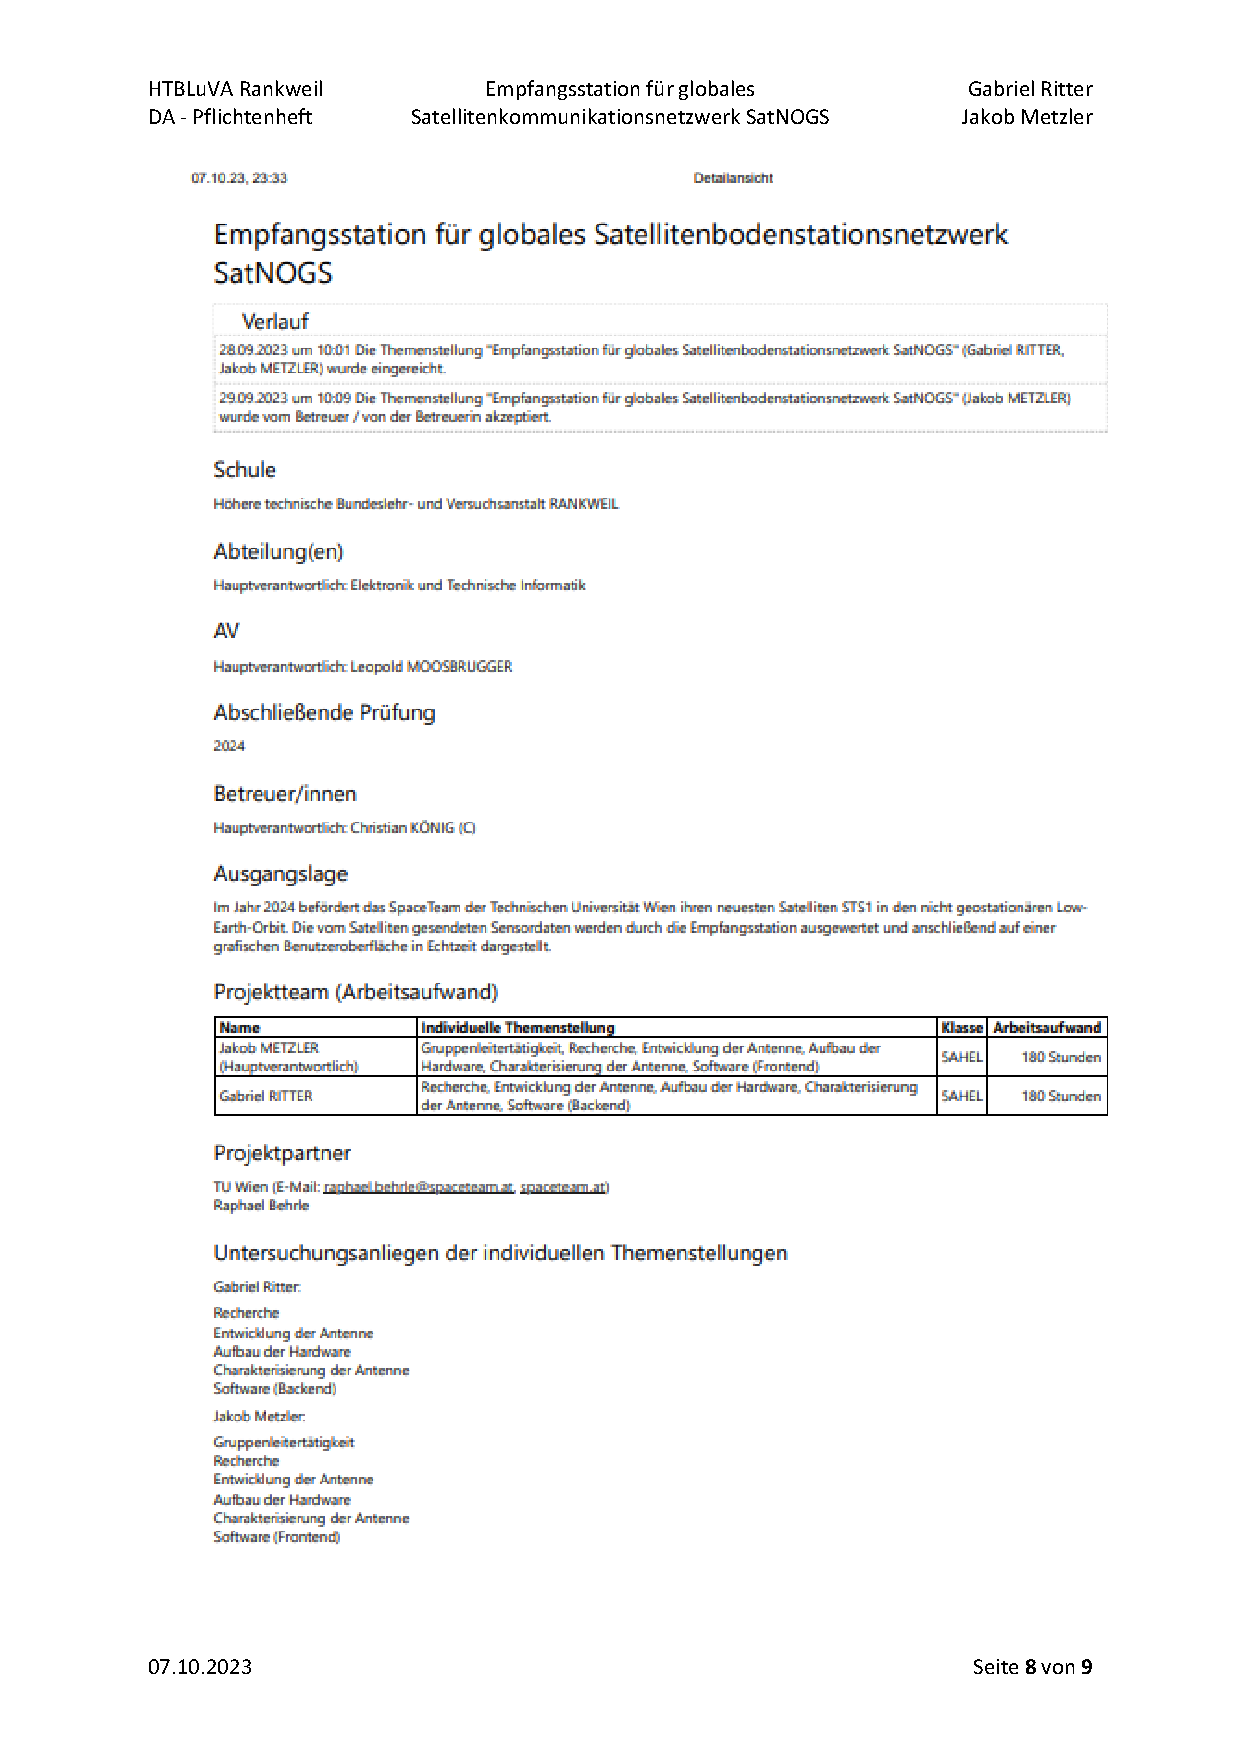
\includegraphics[width=\textwidth]{../ref/DA_Metzler_Ritter_Pflichtenheft_v1.2-page8.pdf}
\end{figure}

\begin{figure}
	\centering
	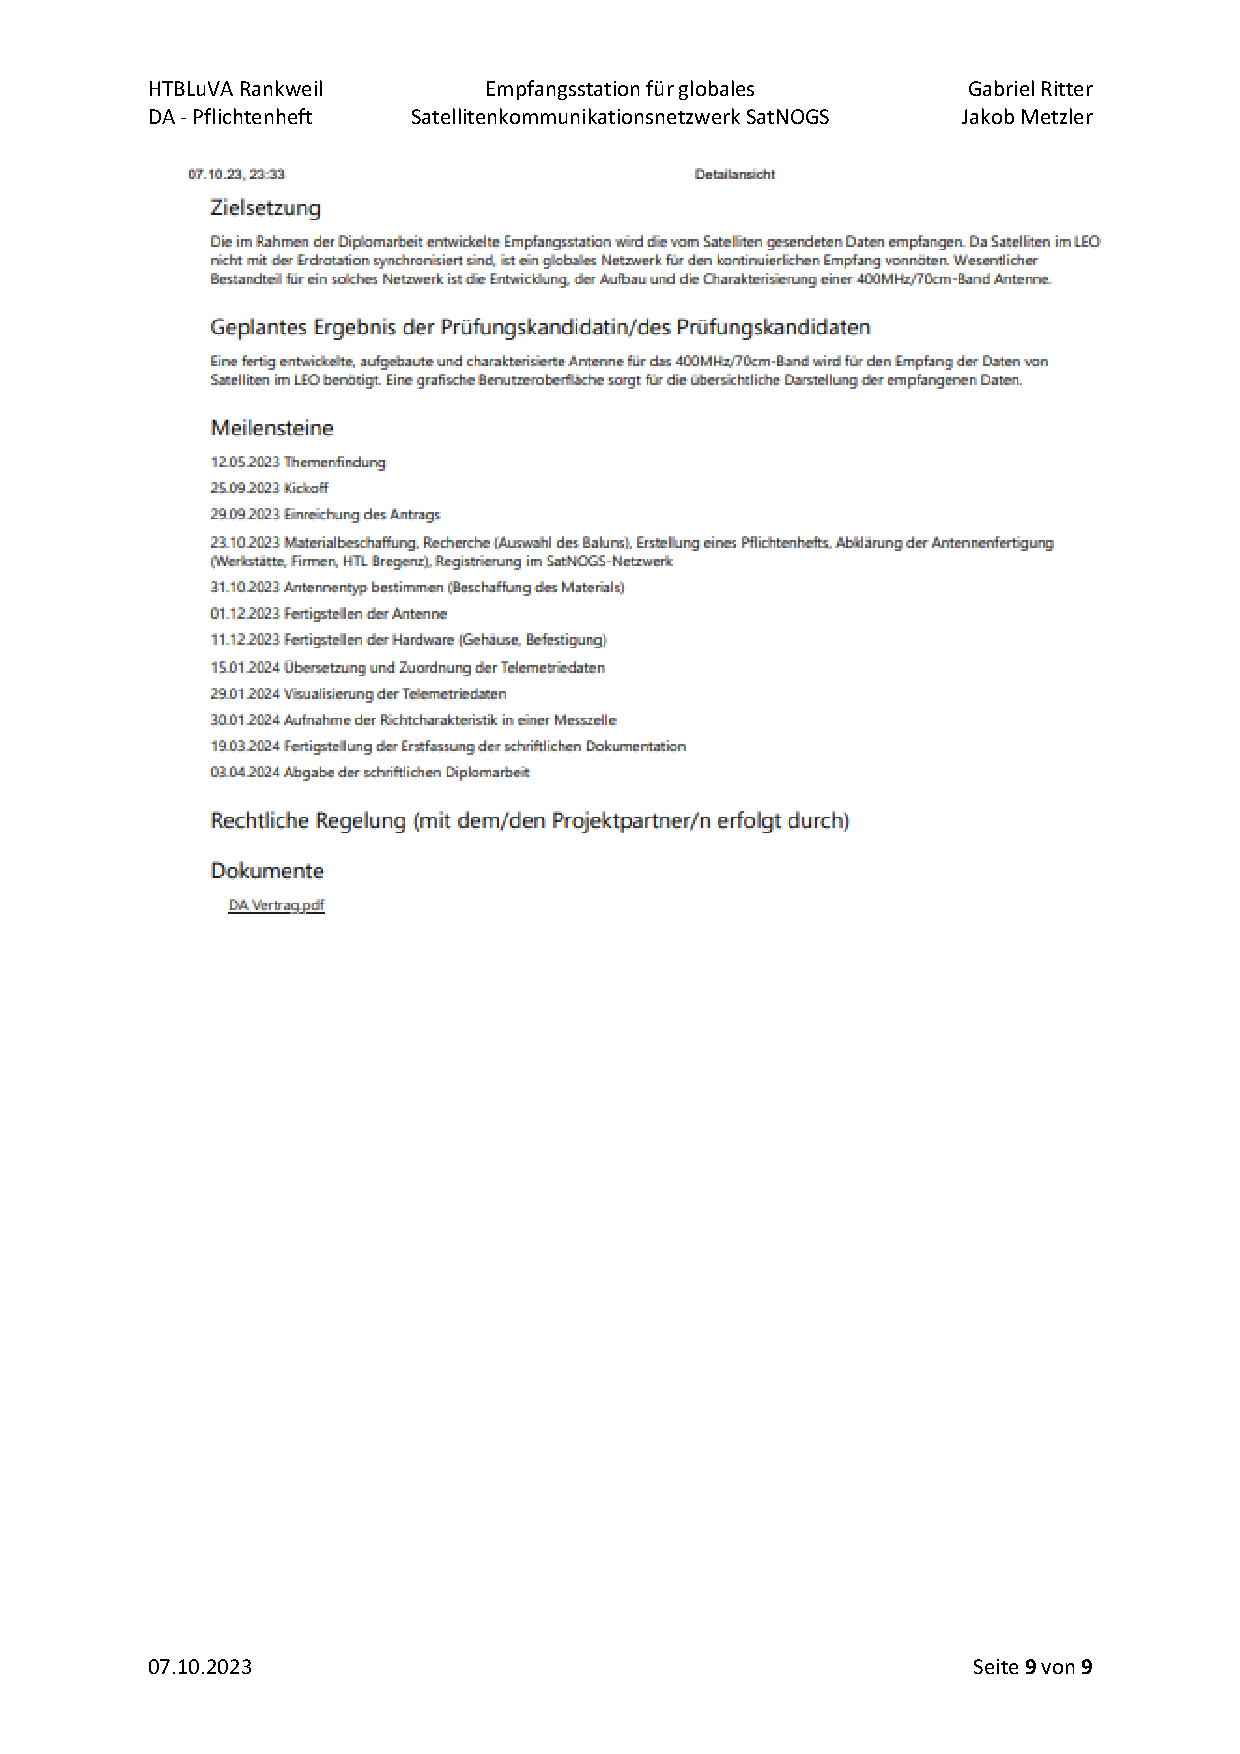
\includegraphics[width=\textwidth]{../ref/DA_Metzler_Ritter_Pflichtenheft_v1.2.-page9pdf.pdf}
\end{figure}


\pagebreak

	\newpage
	
	\SecAuth{\emplLastA, \emplLastB}
	\fancyfoot[LO,RE]{\DADate~\textbar~SatNOGS-Bodenstation~\textbar ~\@SecAuth}
	
	\vspace*{4cm}

\begin{figure}[H]
	
\includegraphics[width=4cm, left]{figures/upper-quote-marks.png}
\end{figure}

\textit{$"$In der Welt der drahtlosen Kommunikation sind Antennen die Stimme, die ohne Worte spricht, aber dennoch eine universelle Sprache vermittelt."} \\
\newline
\rightline{Unbekannt} \\
\vspace{2cm}
\newline
\textit{"Von Anfang an übertraf Maxwells Theorie alle anderen an Eleganz und an der Vielzahl der Beziehungen zwischen den verschiedenen Phänomenen, die sie einschloss."}\\
\newline
\rightline{Heinrich Hertz}
\vspace{1cm}

\begin{figure}[H]
	
\includegraphics[width=4cm, right]{figures/lower-quote-marks.png}
\end{figure}




        % INCLUDE Quotes
	\newpage
	
	% -------------------------- 
	% Main matter
	% --------------------------
	\setcounter{page}{1}			% set page counter
	%\pagestyle{maincontentstyle} 	% fancy header and footer

	\SecAuth{\emplLastB}
	\fancyfoot[LO,RE]{\DADate~\textbar~SatNOGS-Bodenstation~\textbar ~\@SecAuth}
	\chapter{Einführung}

\label{chap:Einführung}
In diesem Kapitel werden die theoretischen Grundlagen der Antennen-und Leitertheorie gelegt sowie das SatNOGS Netzwerk näher erläutert.

\section{SatNOGS-Netzwerk}
\label{sec:sat}
Das SatNOGS-Netzwerk spielt eine zentrale Rolle in unserer Diplomarbeit und bietet hunderten Forschern, Amateurfunkern und Interessierten eine Plattform für verlässliche Kommunikation mit Satelliten.\\

Das, was SatNOGS zu so einer attraktiven Lösung macht, ist der Fakt dass die Bodenstation um den ganzen Globus verteilt sind. Der große Vorteil davon ist, dass der Empfang von Satellitendaten nun über alle verfügbaren Empfangsstationen laufen kann.\\

In Abbildung \ref{fig:SatNOGS_Erklärung} wird die Topologie des SatNOGS-Netzwerkes abstrahiert dargestellt.
Alle über das Netzwerk verfügbaren Bodenstationen sind mit SatNOGS-Servern verbunden. Auf diese Server kann über die Website bzw. API zugegriffen werden, welche die empfangenen Satellitendaten für alle Benutzer erreichbar macht.

\begin{figure}[H]
	\centering
	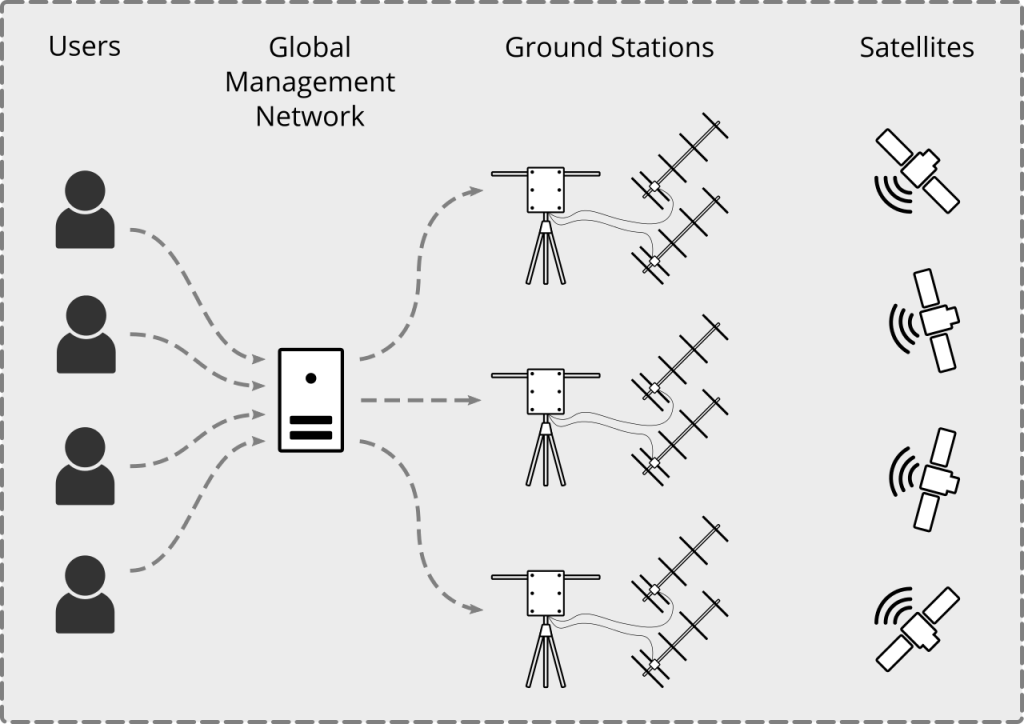
\includegraphics[width=\textwidth]{../ref/SatNOGS_explanation}
	\caption{Erklärung des SatNOGS Netzwerkes}
	\label{fig:SatNOGS_Erklärung}
\end{figure}	

\begin{figure}[H]
	\centering
	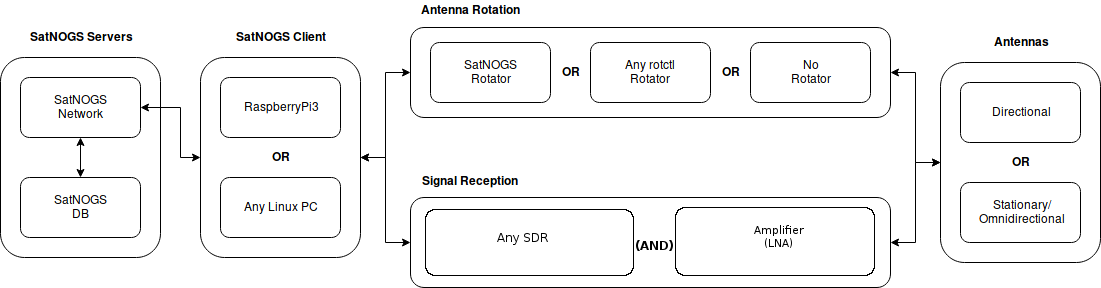
\includegraphics[width=\textwidth]{../ref/SatNOGS_BlockDiagram}
	\caption{SatNOGS-Systemtopologie}
	\label{fig:SatNOGS_Systemtopologie}
\end{figure}

Um näher auf den Ablauf des Datenempfangs und der benötigten Systemblöcke einzugehen wird auf Abbildung \ref{fig:SatNOGS_Systemtopologie} verwiesen.\\

Zum Empfang von Daten kommen zwei Antennentypen infrage: Direktionale oder omnidirektionale Antennen. Eine direktionale Antenne folgt dem Verlauf des Satelliten. Dies bringt den Vorteil mit sich, dass eine höhere Empfangsleistung erzielt, und somit klarere Daten empfangen werden, jedoch wird für solch ein Modell ein Rotator benötigt. Der Vorteil einer omnidirektionalen Antenne ist, dass kein teurer Rotator notwendig ist, allerdings können damit nur schwer brauchbare Daten empfangen werden.\\

Für gerichtete Antennen können verschiedene Rotatoren benutzt werden, unter anderem der "SatNOGS-Rotator" sowie diverse Open-Source-Rotatoren und Rotatoren welche zum Verkauf stehen.\\

Zur Demodulation der Daten sind ein SDR (Software Defined Radio) sowie ein LNA (Low Noise Amplifier) notwendig. Das SDR übernimmt softwaretechnisch Aufgaben welche normalerweise von Hardware übernommen werden (Demodulation, Filter, Mixer, etc...). Der LNA, wie der Name schon andeutet, ist für die Verstärkung kleiner Signale mit besonderer Rauscharmut verantwortlich. \\

Die Aufgabe des SatNOGS Clients kann in der Regel von jedem Linux-PC oder RaspberryPi übernommen werden. Allerdings wird die Kompatibilität zwar für alle Linux-basierten PCs, jedoch nur für die RaspBerryPis Version 3, 3+ und 4 garantiert.\\

Der SatNOGS Client ist mit den Servern verbunden, der die Bodentation als solche im Netzwerk repräsentiert. Die Server unterhalten weiters eine Datenbank, welche Daten über Satelliten enthält, die mit den Empfangsstationen erreichbar sind.
\pagebreak
\section{grundlegende Antennentheorie}
\label{sec:basic-ant}
\subsection{Einführung}
Um die in der Diplomarbeit bearbeiteten Inhalte besser verstehen zu können, wird eine Einführung in die Grundlagen der Antennentheorie gegeben. 

\subsection{Antennenfeldzonen}
Das von einer Antenne abgestrahlte Feld lässt sich in 3 verschiedene Regionen einteilen: das Nahfeld, das Übergangsfeld (Fresnel-Region) und das Fernfeld (Fraunhofer-Region).\\
\newline
Je nach Literatur erfolgt der Übergang zwischen den Feldzonen fließend. Eine Möglichkeit die Zonen einzuteilen ist in der nachfolgenden Tabelle einzusehen.

\begin{center}
	\begin{tabular}[h]{|c|c|c| p{"5"cm}}
		\hline
		Nahfeld & Übergangsfeld & Fernfeld\\
		\hline
		r $<$ 0.2 $\lambda$ & 0.2 $\leq$ r $\leq$ 4$\lambda$ & r $>$ 0.4$\lambda$\\
		\hline
	\end{tabular}
\end{center}

Das Nahfeld ist darin besonders, dass das elektrische und magnetische Feld mit unterschiedlichen Faktoren in Abhängigkeit der Entfernung abnehmen. Im Übergangsfeld nehmen das elektrische und magnetische Feld zwar mit dem gleichen Faktor ab, jedoch unterscheiden Sie sich noch in der Phase und Amplitude.\\
\newline
Im Gegensatz zum reaktiven Nahfeld wird beim Fernfeld Wirkleistung abgestrahlt. Hierbei sind die elektrische und magnetische Komponente der Welle in Phase und nehmen im gleichen Maß ab.\\
\newline
Da unsere Diplomarbeit einen Fokus auf die Satellitentechnik hat, ist für dieses Dokument nur das Fernfeld relevant. 

\subsection{Polarisation}
Die Polarisationsart wird von der Ausrichtung des Vektors der elektrischen Feldstärke bestimmt. Es lässt sich zwischen drei verschiedenen Arten der Polarisation unterscheiden.\\
\newline

\begin{itemize}
	\item Lineare Polarisation
	\begin{itemize}
		\item horizontale Polarisation\\
		Eine horizontale Polarisation liegt vor, wenn der elektrische Feldstärkevektor sich periodisch ändert und die Feldlinien parallel zum Boden verlaufen.
		\item vertikale Polarisation\\
		Eine vertikale Polarisation liegt vor, wenn die elektrischen Feldlinien senkrecht zum Erdboden liegen.
		Eine vertikale Polarisation liegt vor wenn
	\end{itemize}
	\item Zirkulare Polarisation\\
	Der Betrag des elektrischen Feldstärkevektors ist konstant. Der Feldstärkevektor rotiert in einer Spirale um den in Ausbreitungsrichtung weisenden Vektor. Ein Spiralumlauf ist nach der Wellenlänge $\lambda$ vollendet.
	\item Elliptische Polarisation\\
	Betrag sowie Richtung des elektrischen Feldstärkevektors ändern sich laufend. Bei der Rotation beschreibt der Vektor eine Ellipse.
\end{itemize}
linear (vertikal, horizontal), Zirkular, Elliptisch

\subsection{Kenngrößen einer Antenne}
abc

\subsection{Antennengewinn}
Als Antennengewinn wird die $"$bündelnde$"$ Eigenschaft einer gerichteten Antenne im Vergleich zu einer Bezugsantenne bezeichnet. Hierbei ist die Vergleichsantenne meist ein Kugelstrahler.\\
\newline
Der Gewinn der Antenne berechnet sich mit dem Verhältnis der maximalen Empfangsleistung der gerichteten Antenne zu der des Kugelstrahlers. Wird als Bezugsantenne der Kugelstrahler verwendet, so wird die Empfangsleistung mit dem Index 'i' versehen um dies zu kennzeichnen.

\begin{equation}
	G=\frac{P_{max}}{P_{i}}
\end{equation}

\paragraph{Welligkeit}
Die Welligkeit oder das Stehwellenverhältnis (SWR) gibt Aufschluss über die Spannungsverteilung auf der Speiseleitung und ist ein Maß für die Qualität der Anpassung. Sie beschreibt, wie groß der Anteil der reflektierten Wellen ist. Je schlechter die Anpassung, desto größer der Anteil der Wellen, welche reflektiert werden.\\
\newline
\begin{equation}
	SWR=\frac{U_{max}}{U_{min}}=\frac{I_{max}}{I_{min}}=\frac{1+\lvert \rho \lvert}{1-\lvert \rho \lvert}
\end{equation}

Wobei $\rho$ der Reflexionsfaktor ist. 

\paragraph{Richtcharakteristik und Richtdiagramm}
Die Richtcharakteristik beschreibt das Abstrahlverhalten einer Antenne. Hierbei wird die unter einem bestimmten Winkel ($\theta$, $\phi$) auftretende Feldstärke auf einen Maximalwert bezogen.

\begin{equation}
	C(\theta, \phi)=\frac{E(\theta, \phi)}{E_{max}}
\end{equation}

Wobei $\theta$ der Elevationswinkel (vertikal Winkel) und $\phi$ den Azimutwinkel (horizontaler Winkel) repräsentiert.

\begin{figure}[H]
	\centering
	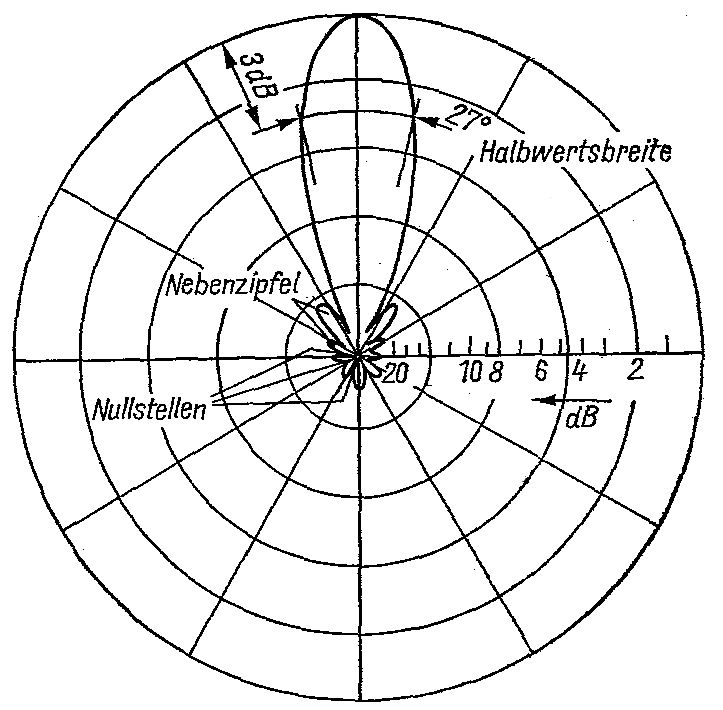
\includegraphics[width=\textwidth]{../ref/Richtdiagramm_Beispiel}
	\caption{Richtdiagramm einer stark bündelnden Antenne}
	\label{fig:Richtdiagramm Beispiel}
\end{figure}

Hierbei ist zu bemerken dass in Abbildung \ref{fig:Richtdiagramm Beispiel} entgegen der üblichen Konvention das Richtdiagramm aus dem Verhältnis zwischen Strahlungsleistungsdichte und ihrem Maximalwert ergibt. Es ist gebräuchlich, das Diagramm auf den Maximalwert zu normieren, sodass sich bei der maximalen Feldstärke 0 dB Dämpfung ergeben.\\
\newline
Der größte Teil der Leistung ist naheliegend in der Hauptkeule zu finden, während es nötig ist die Neben-und Rückwärtskeulen möglichst klein zu halten, um unnötige Abstrahlung in die Umgebung zu vermeiden. Die Halbwertsbreite der Hauptkeule ist der Wert ab dem die Leistungsdichte auf die Hälfte abgesunken ist.\\
\newline
Eine weitere wichtige Kenngröße bei Richtantennen ist das Vor-Rückwärtsverhältnis. Dies ist die Fähigkeit einer Richtantenne, Strahlung aus anderen Richtungen als der Hauptstrahlrichtung zu unterdrücken.

\paragraph{Einfluss der Erde auf das Richtdiagramm}
Wird das Strahlungsdiagramm einer Antenne über dem Boden mit dem einer Antenne im Freiraum verglichen, lassen sich große Unterschiede erkennen. Der Boden dient als Reflektor wobei seine Reflexionseigenschaften von der Dielektrizitätskonstante sowie der Leitfähigkeit bestimmt werden.\\
\newline
Für die Reflexion elektromagnetischer Wellen am Erdboden trifft das Reflexionsgesetz zu, das bedeutet, dass der Einfallswinkel gleich dem Ausfallswinkel ist. Hierbei kann es zu Überlagerungen zwischen den reflektierten und nicht reflektierten Wellen kommen und somit können destruktive und konstruktive Interferenzen entstehen.\\
\newline
Die Polarisierung der verwendeten Antenne spielt eine entscheidende Rolle bei der Reflexion. Bei einer vertikal polarisierten Antenne ist der Stromverlauf von Spiegelbild und Original gleichphasig. Bei einer horizontal polarisierten Antenne hingegen ist der Stromverlauf zwischen Reflexion und Original gegenphasig.\\
\newline
Der Abstand vom Boden spielt ebenfalls eine kritische Rolle und hat großen Einfluss auf das resultierende Richtdiagramm der Antenne. Wird beispielsweise ein Dipol $\frac{\lambda}{2}$ vom Boden entfernt aufgestellt, so verändert sich sein Richtdiagramm so sehr, dass aus der omnidirektionalen Antenne ein Strahler mit zwei Strahlungskeulen wird. 


\subsubsection{Baluns}

\paragraph{Strombalun}
Mantelwellensperre, schwach gegen statische Entladungen, da Balun -> konvertiert balanced zu unbalanced 

\paragraph{Spannungsbalun}
Konvertiert "balanced" zu "unbalanced" guter Schutz gegen statische Entladung, keine Mantelwellensperre.


\section{QHA (Quadrifilare Helixantenne)}
Die QHA ist eine symmetrische Antenne, was bedeutet, dass sie mithilfe eines Baluns auf ein unsymmetrisches Koaxialkabel angepasst werden muss. Mehr dazu in der Subsektion \ref{subsec:baluns}.\\

Die QHA besteht aus einer größeren Schleife, welche unterhalb der gewollten Frequenz resonant ist, und einer kleineren Schleife, welche oberhalb der gewollten Frequenz resonant ist. Die größere Schleife bildet die kapazitive Komponente und die kleinere Schleife die induktive Komponente. Dadurch entsteht eine Phasenverschiebung von (ideal) 90° über die bifilaren Elemente. Werden die Streifen richtig dimensioniert, so ergibt sich eine gute zirkulare Polarisation, weichen sie ab so ergibt sich eine elliptische Polarisation.\\

Das, was die QHA für die Satellitenkommunikation so attraktiv macht, ist zum einen ihre zirkulare Polarisation, und zum anderen ihre kompakte Bauweise. Diese macht sie einfach transportierbar. Zudem hat sie omnidirektionale Abstrahlcharakteristiken, was den Einsatz eines Rotors nichtig macht. Da die QHA entlang des Horizonts ihren größten Antennengewinn aufweist, macht sie das zu einer guten Wahl für die Weltraumkommunikation\cite{qfh_w3kh_nodate}.

\section{Monofilare Helixantenne}
Die Helixantenne ist die in der Satellitenkommunikationstechnik die am Weitesten verbreitete Antennenart \cite{HelicalAntennas}. Der Grund hierfür ist die Immunität der zirkularen Polarisation gegenüber Faraday Rotation. Dieses Phänomen findet in der Ionosphäre statt MISSING REFERENCE und wurde in (REFERENZ) bereits näher erklärt.

Die Helixantenne hat weiters verschiedene Operationsmodi. Arbeitet die Antenne im Normal-Modus, so zeigt sie ein omnidirektionales Abstrahlverhalten, wobei sie senkrecht zur Achse der Antenne gleichmäßig in alle Richtungen strahlt. Dieser Betriebsmodus wird erreicht, sobald der Umfang einer Windung der Helix im Vergleich zu der Wellenlänge $\lambda=\frac{c}{f}$ klein ist. Der zweite Modus der Wendelantenne ist der Axial-Modus. Befindet sich die Antenne in diesem Betriebsverhalten, so verändert sich die Richtung der Strahlung. Der Großteil der elektromagnetischen Strahlung wird nun entlang der Achse der Spirale abgegeben. Dieser Modus wird erreicht, sobald die Wellenlänge ungefähr gleich groß ist wie der Umfang einer Windung der Spirale \cite{HelicalAntennas}.

Da die Wendelantenne über eine besonders große Bandbreite verfügt, eignet sie sich gut für den Nachbau. Hierbei sind der Durchmesser sowie die Steigung der Spirale von ausschlaggebender Relevanz für die gewünschte Einsatzfrequenz. Der Durchmesser für eine Wendelantenne im Axial-Modus ist hierbei mit $D=\frac{\lambda}{\pi}$ definiert.

Ein Richtwert für die Steigung der Helix ergibt sich empirisch mit einem Steigungswinkel zwischen 12° und 14° \cite{helixWebsite}. Die Steigung der Spirale ist so wichtig für die Funktionalität der Antenne, da sie sich mit einem größeren Winkel eher wie ein Dipol verhält, und mit einem kleineren Winkel eher wie eine Ringantenne. REFERENZ

Die folgenden Bezeichnungen werden zur Beschreibung der Helix verwendet.
\begin{itemize}
	\item D: Durchmesser der Helix
	\item S: Abstand zwischen den einzelnen Windungen
	\item U: Umfang der Helix
	\item $\alpha$: Steigung der Helix
	\item L: Länge einer Windung
	\item n: Anzahl der Windungen
	\item Lges: Gesamtlänge der Helix
	\item d: Durchmesser des Leiters
\end{itemize}

Um den Winkel zu berechnen, lässt sich die aufgerollte Windung der Helix betrachten (Abbildung \ref{fig:Wndg_aufgerollt}).

\begin{figure}[H]
	\centering
	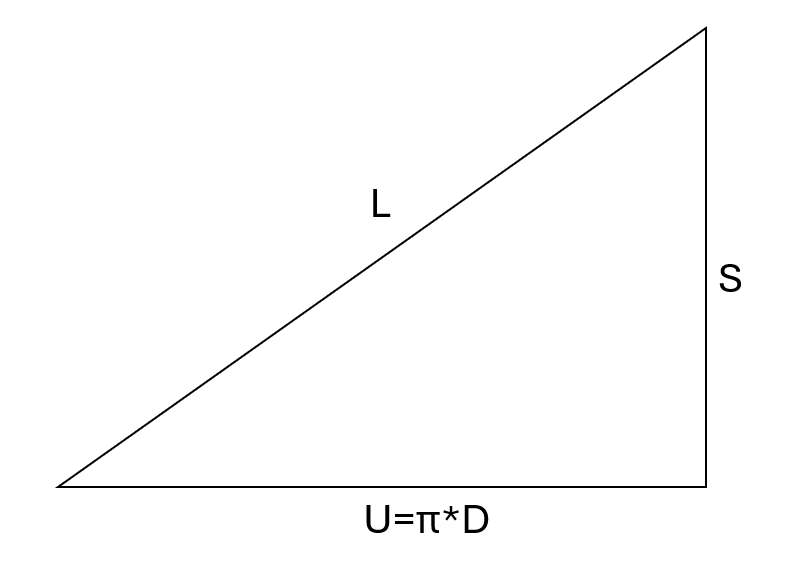
\includegraphics[width=6cm]{../ref/Windung_aufgerollt.png}
	\label{fig:Wndg_aufgerollt}
\end{figure}

Hier lässt sich ein rechtwinkliges Dreieck erkennen. Die Ankathete ist hierbei der Umfang einer Windung und die Gegenkathete stellt den Abstand zwischen den einzelnen Drehungen dar. Somit lässt sich der Winkel $\alpha$ mit der Formel

\begin{equation}
	\alpha=\arctan(\frac{S}{C})
\end{equation}

beschreiben. Ein weiterer vitaler Parameter für die Funktionalität der Antenne ist der Abstand zwischen den einzelnen Windungen. Dieser wird generell für $0,23\lambda$ als ideal angegeben. MISSING REFERENCE

Der Reflektor dient zur Verbesserung der Richtcharakteristik und kann verschiedene Formen annehmen. Er kann kreisförmig, viereckig oder auch trichterförmig sein. Für die Zwecke dieser Diplomarbeit wurde ein kreisförmiger Reflektor gewählt. Als passend wird hierbei ein Durchmesser zwischen $\frac{3\lambda}{4}$ und $\frac{4\lambda}{3}$ angesehen. Der Durchmesser des Leiters ist unkritisch für die Funktion der Antenne, allerdings wird als Richtwert ein Querschnitt von $0,005\lambda$ bis $0,05\lambda$ als passend betrachtet\cite{Kraus-2002-AntennasB}. 

Nachfolgend sind die wichtigsten Gleichungen für die Berechnung der Parameter einer Helix-Antenne gegeben \cite{Kraus-2002-AntennasB}.

\begin{table}[H]
	\begin{tabular}{|l|l|}

		\textbf{Bezeichnung} & \textbf{Formel}\\ 
		benötigte Kabellänge & $L=n*\sqrt{\lambda^2+S^2}$ \\
		D				     & $D=\frac{\lambda}{\pi}$\\ 
		Halbwertsbreite		 & $HPBW=\frac{52}{C*\sqrt{nS}}$ \\ 
		Gewinn               & $G=12*C^2nS$                 \\ 
		Eingangsimpedanz     & $Z=\frac{150}{\sqrt{C}}$      \\ 
		Effektive Antennenfläche    & $Ae=\frac{D*\lambda^2}{4*\pi}$ \\ 
		\end{tabular}
	\end{table}

Anhand der Formel für den Antennengewinn lässt sich erkennen, dass dieser direkt proportional zur Anzahl an Windungen ist. Die Antennenwirkfläche beschreibt, welche Leistung dem elektromagnetischen Feld bei bekannter Leistungsdichte entnommen wird, wie bereits in QUERVERWEIS erwähnt MISSING REFERENCE.

 % INCLUDE Introduction
	\newpage
	\SecAuth{\emplLastA}
	\fancyfoot[LO,RE]{\DADate~\textbar~SatNOGS-Bodenstation~\textbar ~\@SecAuth}
	\chapter{Einrichten des SatNOGS Client}
\label{chap:gs-setup}
Der SatNOGS Client bildet das Herzstück der gesamten Empfangsstation, ist für die Ausführung und Koordinierung der, mit der Empfangstation geplanten, Observationen zuständig und bildet die Schnittstelle zur SatNOGS Datenbank. Das SatNOGS-Client Script kann auf einer beliebigen Linux Distribution installiert und ausgeführt werden. Für die, wie in diesem Fall, Anwendung eines Raspberry Pi 4  Einplatinencomputers zur Ausführung des Client Scripts empfiehlt sich, dass speziell für den SatNOGS Client entwickelte Raspbian SatNOGS Image, zu verwenden. Dieses angepasste Image für das Raspbian Betriebssystem sorgt dafür, dass alle benötigten Softwarepakete und das SatNOGS setup script vorinstalliert vorinstalliert sind und der SSH-Server auf dem Raspberry Pi 4 aktiviert wird. Auf die Installation wird nicht näher eingegangen sondern auf die Anleitung im SatNOGS Wiki \cite{noauthor_raspberry_nodate} verwiesen. 

\section{grundlegende Konfiguration}
\subsection{Verbinden zum Raspberry PI 4}
Um Einstellungen am Raspberry Pi 4 vornehmen zu können wird auf diesen über SSH zugegriffen. Dazu muss das Gerät welches auf den Raspberry Pi 4 zugreift am besten mit dem selben Netzwerk verbunden sein wie der Raspberry selbst. Die einfachste Vorgehensweise um sich mit dieser Voraussetzung zum Raspberry Pi 4 über SSH zu verbinden, besteht mit einem Windows System darin, in der Eingabeaufforderung den Befehl \textbf{ssh *hostname*} auszuführen. Der Hostname wird im Zuge der Installation des Betriebssystems vergeben und lautet in diesem Fall \textbf{qfh}. Wurde ein Passwort im Zuge der Installation eingegeben, so erscheint anschießend eine Aufforderung dieses einzugeben. Nach der Eingabe wird bei erfolgreicher Verbindung folgende Information zurückgegeben:

\begin{figure} [H]
	\centering
	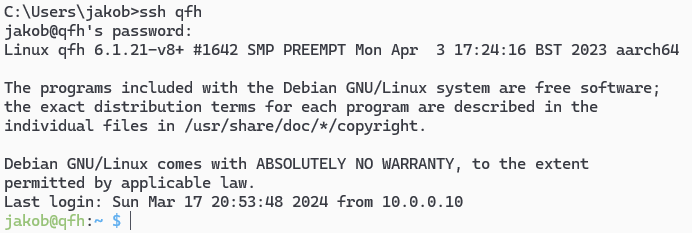
\includegraphics[width=\linewidth]{../ref/successfull_login.png}
	\caption{Erfolgreiche Verbindung über SSH}
	\label{fig:htrl-uhf(test)successfulllogin}
\end{figure}

\subsection{Hauptmenü}
Mithilfe des Befehls \textbf{sudo satnogs-setup} öffnet sich das Hauptmenü des SatNOGS Client über welches alle Einstellungen vorgenommen werden können.

\begin{figure} [H]
	\centering
	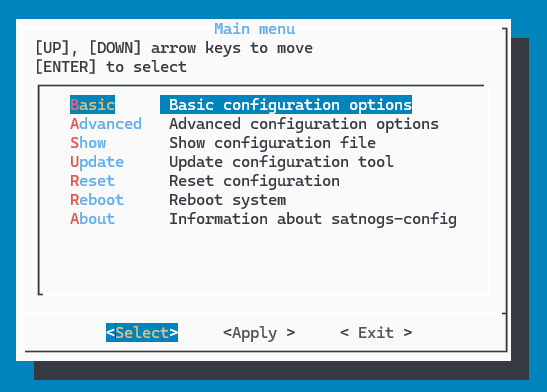
\includegraphics[width=.5\linewidth]{../ref/mainmenu.png}
	\caption{SatNOGS Client: Hauptmenü}
	\label{fig:mainmenu}
\end{figure}

Wurden alle Einstellungen vorgenommen so können diese mit \textbf{Apply} angewendet und gespeichert und angewendet werden.

\subsection{Einstellungen}
Wird im Hauptmenü der Reiter \textbf{Basic} mit \textbf{Enter} ausgewählt, so erscheint folgendes Fenster über welches alle grundlegenden Einstellungen zum Betrieb einer Empfangsstation vorgenommen werden können.

\begin{figure} [H]
	\centering
	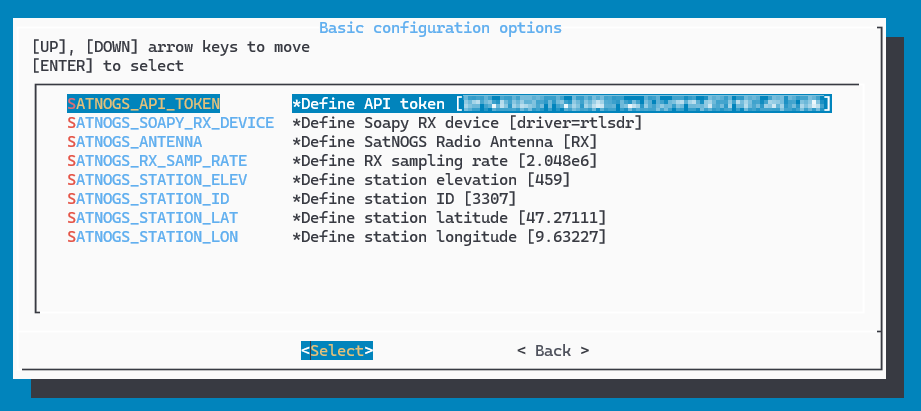
\includegraphics[width=.75\linewidth]{../ref/basic_configurations.png}
	\caption{SatNOGS Client: grundlegende Einstellungen}
	\label{fig:basic_configurations}
\end{figure}

\subsubsection{SATNOGS\textunderscore API\textunderscore TOKEN}
Der API-Schlüssel, welcher mit dem SatNOGS-Benutzerkonto verknüpft ist, wird von der Empfangsstation benötigt sich gegenüber der SatNOGS-Datenbank zu identifizieren und authentifizieren. Er kann auf dem Benutzerprofil der SatNOGS-Netzwerk Webseite durch das Klicken auf den in der folgenden Grafik mit 1 markierten Button an der mit 2 markierten Stelle abgelesen werden.

\begin{figure} [H]
	\centering
	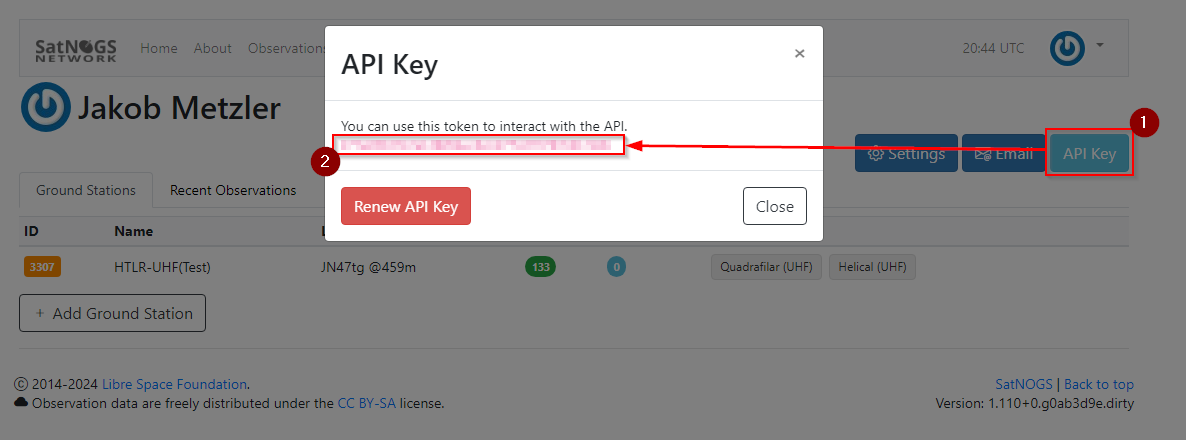
\includegraphics[width=.75\linewidth]{../ref/apitoken.png}
	\caption{SatNOGS-Netwerk Homepage: API-Schüssel ermitteln}
	\label{fig:apikey}
\end{figure}

\subsubsection{SATNOGS\textunderscore SOAPY\textunderscore RX\textunderscore DEVICE}
Mithilfe dieses Einstellungsparameters wird dem SatNOGS Client das verwendete SDR mitgeteilt. In diesem Fall entspricht das SDR dem, im späteren Kapitel \ref{sec:sdr} genauer Erläuterten, RTL-SDR Blog v3 und die dementsprechende einzugebende Treiber-Kennzeichnung lautet \textbf{driver=rtlsdr} \cite{noauthor_satnogsclient_nodate}. Weitere Treiber-Kennzeichnungen können auf der Software Defined Radio Seite des SatNOGS Wiki \cite{noauthor_software_nodate} nachgeschlagen werden.

\subsubsection{SATNOGS\textunderscore ANTENNA}
Über diesen Einstellungsparameter wird entsprechend dem verwendeten SDR und dem passenden Parameter der Modus des SDRs konfiguriert. Für das RTL-SDR Blog v3 entspricht das dem Parameter \textbf{RX} \cite{noauthor_satnogsclient_nodate}. Entsprechende Parameter für weitere SDR Typen können auf der Software Defined Radio Seite des SatNOGS Wiki \cite{noauthor_software_nodate} nachgeschlagen werden. 

\subsubsection{SATNOGS\textunderscore RX\textunderscore SAMP\textunderscore RATE}
Dieser Parameter legt die Abtastrate des SDRs fest. Für das RTL-SDR Blog v3 wird eine Abtastrate von 2.048 Megasamples pro Sekunde empfohlen \cite{noauthor_satnogsclient_nodate}, was über den Parameter 2.048e6 eingestellt werden kann. Auch hier finden sich für andere SDRs Informationen auf der Software Defined Radio Seite des SatNOGS Wiki \cite{noauthor_software_nodate}. 

\subsubsection{SATNOGS\textunderscore STATION\textunderscore ELEV}
Für diesen Parameter ist es notwendig die Höhenlage der Empfangsstation zu ermitteln. Es empfiehlt sich dazu eine interaktive topografische Karte, wie de-at.topographic-map.com, zu verwenden. Für den Standort der HTL Rankweil entspricht dieser Wert, was zugleich auch dem Parameter entspricht, 459 Meter. Dieser Wert wird für die Berechnungen der passierenden Satelliten und dessen Elevation- und Azimutalwinkel verwendet.

\subsubsection{SATNOGS\textunderscore STATION\textunderscore ID}
Die Station-ID wird zur eindeutigen Identifikation der Empfangsstation im SatNOGS-Netzwerk verwendet und kann auf der Seite des Benutzerprofils auf der Homepage des SatNOGS-Netzwerks abgelesen werden. 

\begin{figure} [H]
	\centering
	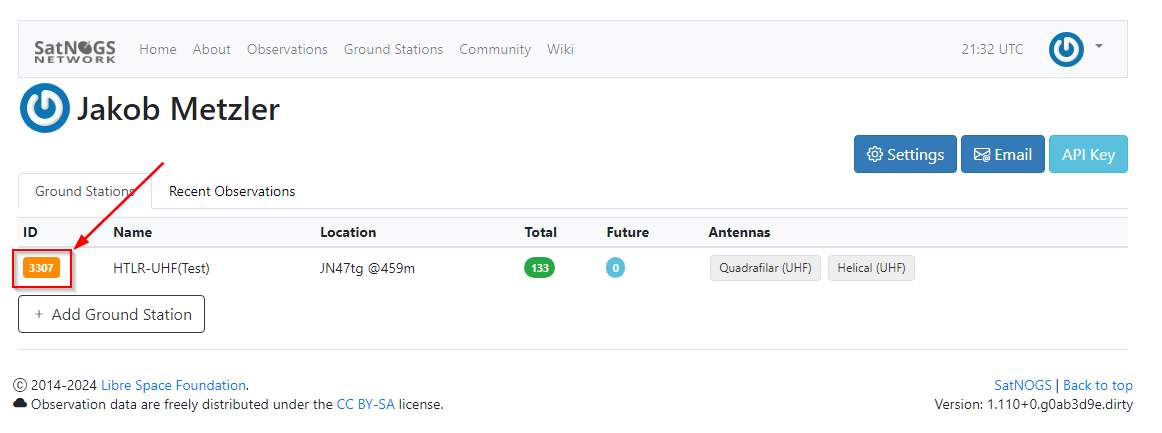
\includegraphics[width=.75\linewidth]{../ref/stationid.png}
	\caption{SatNOGS-Netzwerk Homepage: Station-ID ermitteln}
	\label{fig:stationid}
\end{figure}

\subsubsection{SATNOGS\textunderscore STATION\textunderscore LAT}
Dieser Parameter gibt den Breitengrad der Position der Empfangsstation an. Dieser Wert wird für die Berechnungen der passierenden Satelliten und dessen Elevation- und Azimutalwinkel verwendet.

\subsubsection{SATNOGS\textunderscore STATION\textunderscore LON}
Dieser Parameter gibt den Längengrad der Position der Empfangstation an. Dieser Wert wird für die Berechnungen der passierenden Satelliten und dessen Elevation- und Azimutalwinkel verwendet.

\section{erweiterte Konfiguration} 
Wird im Hauptmenü der Reiter \textbf{Advanced} mit \textbf{Enter} ausgewählt, so erscheint folgendes Fenster über welches erweiterte Einstellungen vorgenommen werden können. 

\begin{figure} [H]
	\centering
	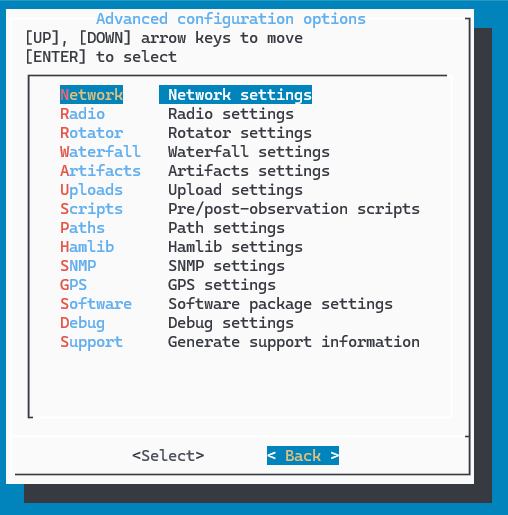
\includegraphics[width=.5\linewidth]{../ref/advanced_settings.png}
	\caption{SatNOGS Client: erweiterte Einstellungen}
	\label{fig:advanced_settings}
\end{figure}

Die wichtigsten Einstellungen die hier vorgenommen werden können sind das definieren der Verstärkung des SDRs, das Einrichten einer Unterstützung für die Verwendung eines Rotors und das automatische Aktivieren von Bias-T während einer Observation.

\subsection{Verstärkung des SDRs einstellen}
Um die Verstärkung des SDRs einzustellen müssen zuerst die möglichen Parameter ermittelt werden, was durch das ausführen des Befehls \textbf{rtl\textunderscore test} in der SSH gemacht werden kann. 

\begin{figure} [H]
	\centering
	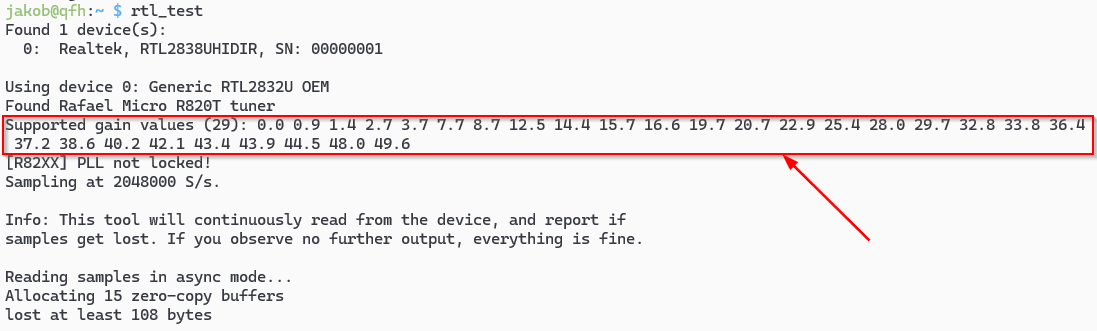
\includegraphics[width=\linewidth]{../ref/supportedgain.png}
	\caption{SatNOGS Client: unterstützte Gain Werte ermitteln}
	\label{fig:supportedgain}
\end{figure}

Wurde aus der Ausgabe, wie in obiger Darstellung gezeigt, der gewünschte Wert der Verstärkung gewählt, so kann dieser in den erweiterten Einstellungen unter dem Reiter \textbf{Radio} mithilfe des Parameters \textbf{SATNOGS\textunderscore RF\textunderscore GAIN} eingestellt werden. 

\subsection{Rotor-Unterstützung implementieren}
Für die Implementierung einer Rotorsteuerung müssen in den erweiterten Einstellungen unter dem Reiter \textbf{Rotator} drei Parameter angepasst werden. 

Der erste Parameter \textbf{SATNOGS\textunderscore ROT\textunderscore ENABLED} aktiviert die Verwendung der konfigurierten Rotorsteuerung. 

Mithilfe des Parameters \textbf{SATNOGS\textunderscore ROT\textunderscore MODEL} wird das Model der Rotorsteuerung festgelegt. Im Fall der im späteren Kapitel \ref{sec:gs232emulation} erläuterten GS232A/B Steuerung wird für den Parameter \textbf{ROT\textunderscore MODEL\textunderscore GS232B} verwendet \cite{noauthor_satnogsclient_nodate}. 

\textbf{SATNOGS\textunderscore ROT\textunderscore BAUD} legt die Baud-Rate der Kommunikation mit der Steuerung fest und beträgt im Fall der im späteren Kapitel \ref{sec:gs232emulation} erläuterten Steuerung 9600.

\subsection{Aktivieren von Bias-T}
Das Aktivieren von Bias-T ist abhängig vom verwendeten SDR und wird nun nur für das RTL-SDR Blog v3 erläutert. Um die softwaremäßigen Voraussetzungen für die Verwendung von Bias-T am RTL-SDR Blog v3 zu erfüllen müssen im ersten Schritt folgende Befehle in der SSH ausgeführt werden:
\newline 1. \textbf{sudo apt install cmake}
\newline 2. \textbf{git clone https://github.com/rtlsdrblog/rtl\textunderscore biast}
\newline 3. \textbf{cd rtl\textunderscore biast}
\newline 4. \textbf{mkdir build}
\newline 5. \textbf{cd build}
\newline 6. \textbf{cmake ..}
\newline 7. \textbf{make}

Diese Schritte ermöglichen die Kontrolle der Bias-T Funktion des RTL-SDR Blog v3 und müssen nur einmal durchgeführt werden. Sie ermöglichen die Kontrolle der Funktion über folgende Befehle:
\newline Einschalten: \textbf{/rtl\textunderscore biast/build/src/rtl\textunderscore biast -b 1}
\newline Ausschalten: \textbf{/rtl\textunderscore biast/build/src/rtl\textunderscore biast -b 0}

Diese Befehle können nun in den erweiterten Einstellungen unter dem Reiter Scripts als Pre- und Post-Observation Script festgelegt werden. Dazu wird der Einschalt- sowie Ausschaltbefehl mit \textbf{/home} am Anfang, aufgrund des Ursprungsverzeichnisses des SatNOGS Client, erweitert werden.		% INCLUDE Groundstation setup
	\newpage
	\SecAuth{\emplLastA}
	\fancyfoot[LO,RE]{\DADate~\textbar~SatNOGS-Bodenstation~\textbar ~\@SecAuth}
	\chapter{Yaesu-G5500 Rotor}
Rotoren werden in der Antennentechnik eingesetzt, um die Kommunikation mit nicht-geostationären Satelliten zu ermöglichen, wobei Antennentypen mit hoher Richtwirkung verwendet werden (z.B. Helix-Antenne). In der Regel wird durch diese Methode eine höhere Verstärkung erzielt, als es mit Antennen möglich ist, die den gesamten Horizont abdecken und daher keine Nachführung erfordern. 
\section{Azimut- und Elevationswinkel}
Die Ausrichtung des Rotors und somit auch die der Antenne wird mithilfe des astronomischen Horizont Koordinatensystems beschrieben. 
	\newpage
	\SecAuth{\emplLastA}
	\fancyfoot[LO,RE]{\DADate~\textbar~SatNOGS-Bodenstation~\textbar ~\@SecAuth}
	\chapter{Quadrifilare Helixantenne (QHA)}
Die Quadrifilare Helixantenne ist eine Abwandlung der monofilaren Helixantenne und unterscheidet sich von dieser in mehreren wichtigen Punkten.

Zum einen ist sie um einiges kleiner als die monofilare Helix. Zum anderen wird sie als omnidirektionale Antenne für Satellitenkommunikation verwendet, da sie, wie die monofilare Helix, zirkular polarisiert ist. Allerdings zeigt sie entlang des Horizonts sowie direkt nach oben einen besseren Antennengewinn als in andere Richtungen.

\section{Funktionsweise}
Die QHA ist eine symmetrische Antenne, was bedeutet, dass sie mithilfe eines Baluns auf ein unsymmetrisches Koaxialkabel angepasst werden muss. Mehr dazu in Kapitel QUERVERWEIS.

Die QFH besteht aus einer größeren Schleife, welche unterhalb der gewollten Frequenz resonant ist, und einer kleineren Schleife, welche oberhalb der gewollten Frequenz resonant ist. Die größere Schleife bildet die kapazitive Komponente und die kleinere Schleife die induktive Komponente. Dadurch entsteht eine Phasenverschiebung von (ideal) 90° über die bifilaren Elemente. Werden die Streifen richtig dimensioniert, so ergibt sich eine gute zirkulare Polarisation, weichen sie ab so ergibt sich eine elliptische Polarisation.

\section{Design}
stl files, beschreibung der form

BILD DER QFH

\section{Realisierung}
Metallstreifen, metallrundlinge

BILD DER QFH

\section{Messungen}
	\newpage
	\SecAuth{\emplLastB}
	\fancyfoot[LO,RE]{\DADate~\textbar~SatNOGS-Bodenstation~\textbar ~\@SecAuth}
	\chapter{Helixantenne}
\label{chap:helix}
Die zweite aufgebaute Antenne ist eine monofilare Helixantenne. Dieser Antennentyp ist gerichtet, was bedeutet, dass sie in eine bestimmte Richtung einen höheren Antennengewinn als in andere Richtungen hat. Sie ist eine der einfachsten Antennenarten um eine zirkulare Polarisation zu erzielen. Kombiniert mit ihrer hohen Bandbreite macht sie das zu einer attraktiven Option zum Nachbau und zur Verwendung in der Satellitenkommunikation\cite{helixWebsite}.

Alle Zeichnungen der in diesem Kapitel vorkommenden Konstruktionen und Baugruppen finden sich in Kapitel \ref{chap:Anhang}.

Für die in dieser Diplomarbeit konstruierte Helixantenne wurden die folgenden Vorgaben gewählt.

\begin{center}
	\begin{tabular}{|c|c|}
	\textbf{Parameter} & \textbf{Wert}\\
	Resonanzfrequenz & 433MHz\\
	Windungen & 6\\
	Abstand zwischen Windungen & $0,25\lambda$\\
	Polarisationsart & RHCP\\
	Betriebsmodus & Axial-Modus
\end{tabular}
\end{center}

Wobei $"$RHCP$"$ $"$Right Hand Circularily Polarized$"$ bedeutet. Für mehr Informationen zur zirkularen Polarisation wird auf den Abschnitt $"$\ref{subsec:pol} Polarisation$"$ verwiesen.

\section{Design}
Durch den Einsatz im Freien muss die Helixantenne einige Anforderungen erfüllen. Beispielsweise dürfen wichtige Strukturelemente unter UV-Einwirkung nicht brüchig werden, es darf sich durch Regen kein Wasser stauen und sie muss starkem Wind standhalten. 

Um die Helixantenne zu designen wurden Online-Rechner verwendet \cite{calculator_daycounter, calculator_jcoppens}.

\begin{center}
	\begin{tabular}{|c|c|}
	\textbf{Parameter} & \textbf{Wert} \\
	Wellenlänge &  692.8mm\\
	Durchmesser (intern) & 235.7mm\\
	Abstand zwischen den Windungen & 173.2mm\\
	Gesamthöhe & 1039.2mm\\
	minimaler Reflektor-Durchmesser & 429.5mm
\end{tabular}
\end{center}

Mithilfe dieser Werte wurde die erste Wendelantenne in Fusion 360 konstruiert. 

\begin{figure}[h!]
	\centering
	\includegraphics[width=5cm]{../ref/Erste Helixnäherung v0.png}
	\label{fig:ersteHelixnäherung}
	\caption{Das CAD-Modell für die Helixantenne mit den berechneten Werten}
\end{figure}

Diese wurde mithilfe von CENOS-Simulation-Suite für einen Frequenzbereich von 400MHz bis 460MHz simuliert. Die Ergebnisse geben Aufschluss über die Performance der Antenne in einer idealen Umgebung.

\begin{figure}[h!]
	\centering
	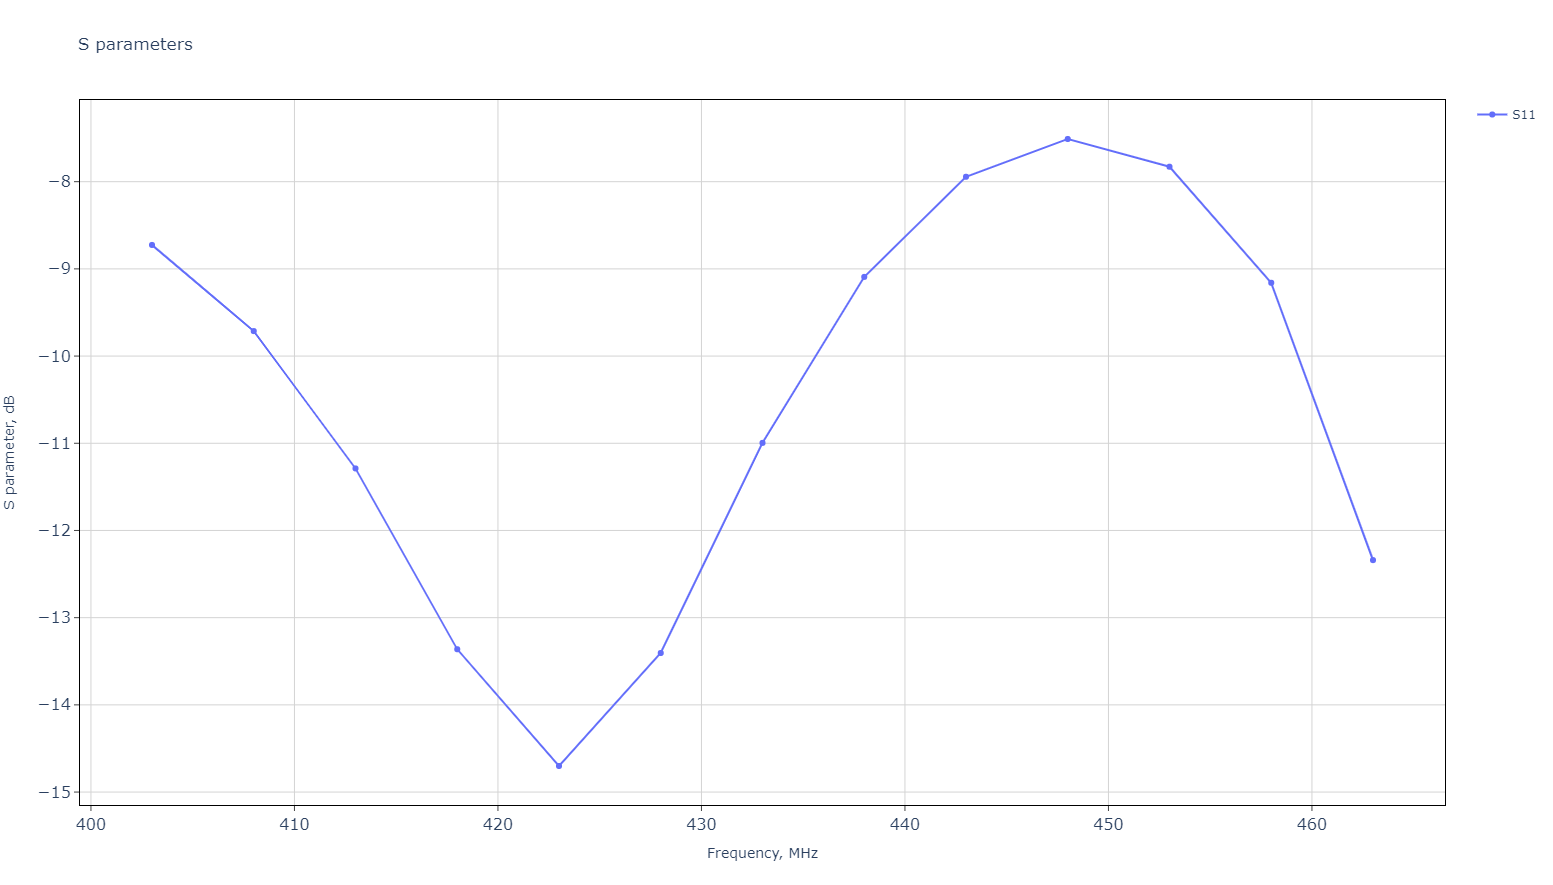
\includegraphics[width=10cm]{../ref/helix-naherung-S11.png}
	\label{fig:ersteHelixnäherung-S11}
	\caption{S11-Parameter der berechneten Helixantenne}
\end{figure}

\begin{figure}[h!]
	\centering
	\includegraphics[width=10cm]{../ref/helix-näherung-radiation-pattern.png}
	\label{fig:ersteHelixnäherung-abstrahldiagramm}
	\caption{Abstrahldiagramm der berechneten Helixantenne}
\end{figure}

Es wurde der Schluss gezogen, dass die Resonanzfrequenz zu weit unter dem gewünschten Wert von 433MHz liegt. Diese lässt sich durch Veränderung des Durchmessers der Spirale oder des Abstandes zwischen den Windungen verändern.

Durch das Abändern des Durchmessers konnte die gewünschte Resonanzfrequenz von 433MHz mit einem Helix-Durchmesser von 270mm erreicht werden. Der Reflektor wurde aus der Theorie mit ca. $\frac{3\lambda}{4}$ festgelegt \cite{Kraus-2002-AntennasB}, was einem Durchmesser von ungefähr 520mm entspricht.

\begin{figure}[H]
	\centering
	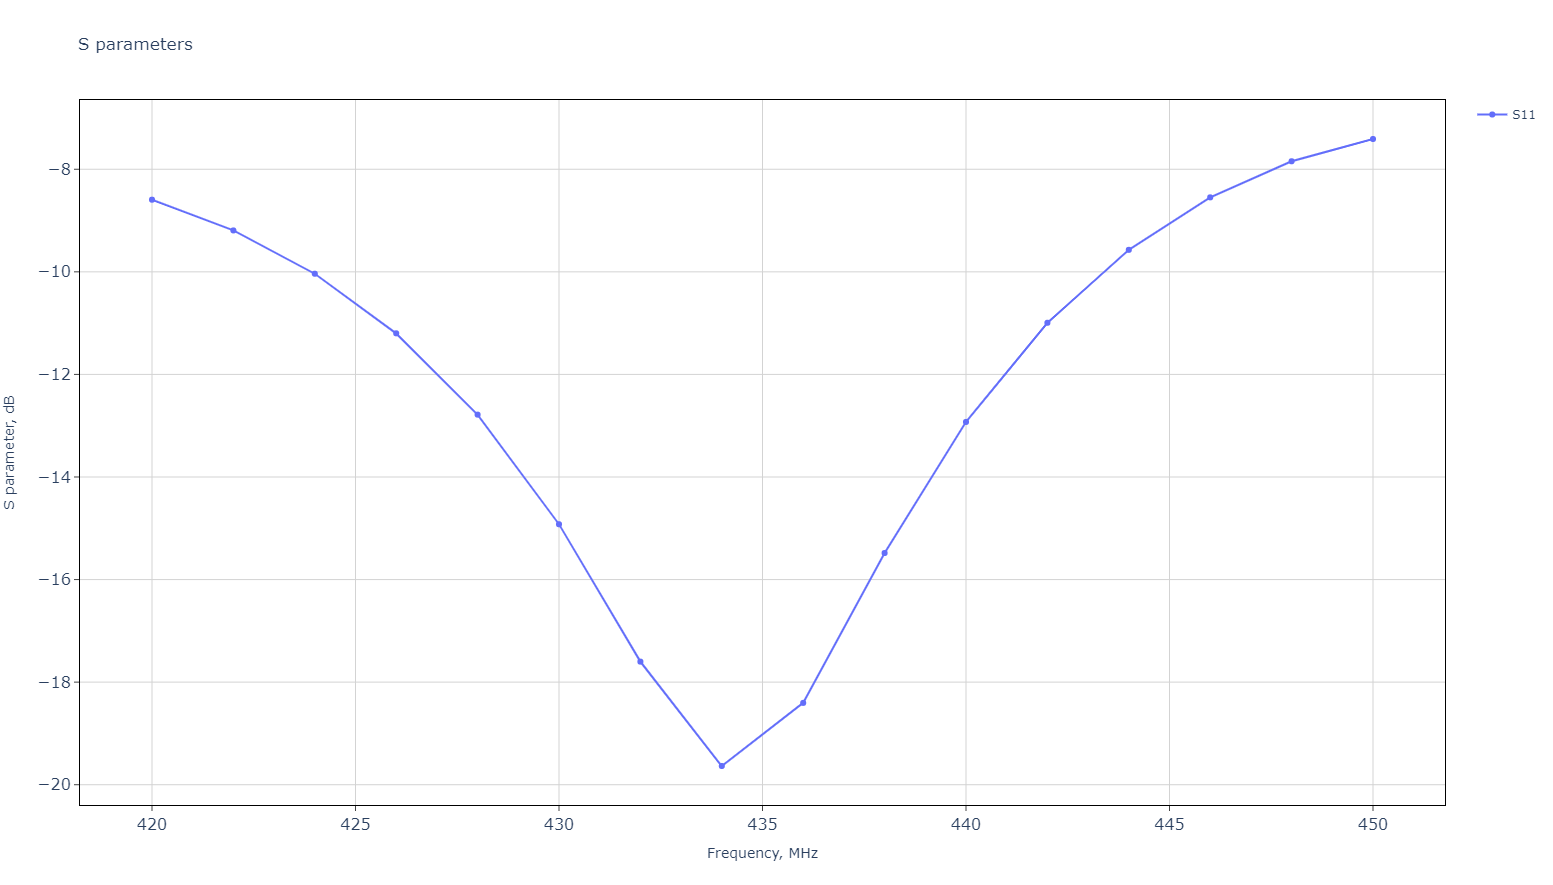
\includegraphics[width=10cm]{../ref/helix-fertig-S11.png}
	\label{fig:fertigeHelix-S11}
	\caption{S11-Parameter der richtig dimensionierten Helixantenne}
\end{figure}

\begin{figure}[H]
	\centering
	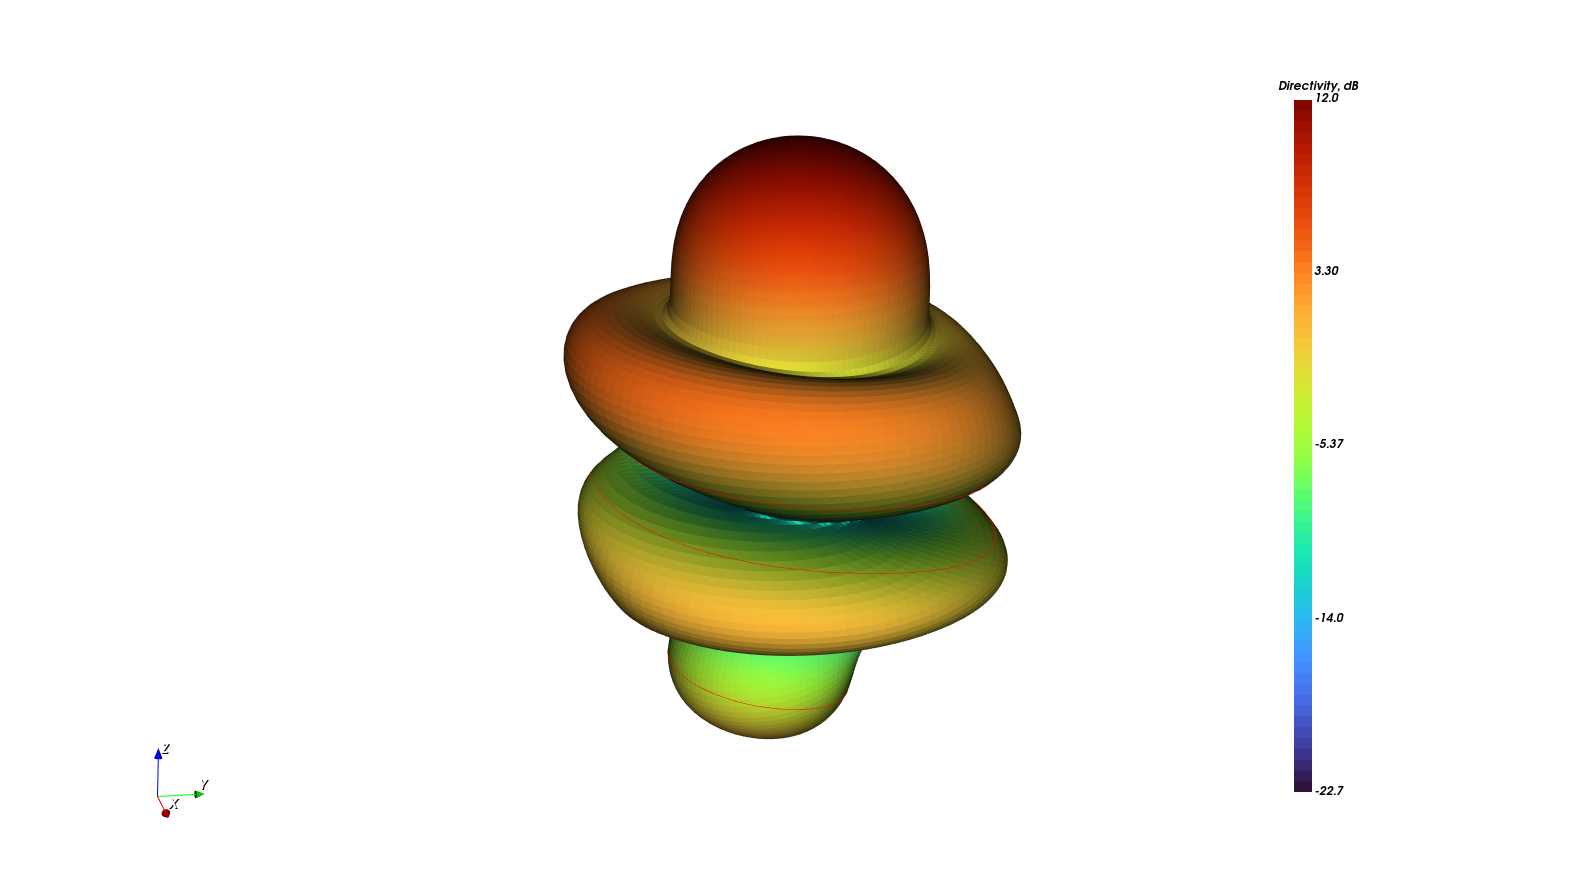
\includegraphics[width=10cm]{../ref/helix-fertig-radiation-pattern.png}
	\label{fig:fertigeHelix-Radiation}
	\caption{Abstrahldiagramm der richtig dimensionierten Helixantenne}
\end{figure}

Es ist wichtig anzumerken, dass der Steigungswinkel der Spirale hierbei ca. 11,5° beträgt. Dies hat zur Folge, dass die Steigung von dem relativ engen Idealbereich zwischen 12° und 14° abweicht.

\section{Realisierung}
Die Helixantenne benötigt zur Funktion nur zwei Bauteile: die Spirale und den Reflektor. Die Antenne funktioniert dann am Besten, wenn diese zwei Bauteile nicht von ihrer Umgebung beeinflusst werden. Hierfür muss darauf geachtet werden dass die Strukturelemente so wenig Kontakt mit der eigentlichen Antenne wie möglich haben. Um den Einfluss der Umgebung weiter zu verringern, werden spezielle Materialien mit einer niedrigen elektrischen Permittivität verwendet, beispielsweise Teflon, um kapazitive Einflüsse gering zu halten. 

\begin{figure}[H]
	\centering
	\includegraphics[width=10cm,angle=270]{../ref/Helixantenne-real.jpg}
	\caption{Reale Helixantenne}
	\label{fig:helix-real}
\end{figure}

\begin{table}
	\begin{tabular}{|c|c|c|c|c|}
	\hline
	Nr. & Typ & Maße & Besonderheiten & Menge \\
	\hline
	1 & PVC-Rohr & 50x3,7mm 1m & UV-stabilisiert & 4x \\
	\hline
	2 & Teflon-Rundlinge & \O 10mm 2m & UV-resistent & 4x \\
	\hline
	3 & PVC-Rohrschelle & toleriert 16-18mm & UV-stabilisiert & 44x \\
	\hline
	4 & Aluminiumrohr & 18x2mm 5,2m & & 4x \\
	\hline
	5 & Runde Aluminiumplatte & \O 520x3mm & & 4x \\
	\hline
	6 & Rohrflansch (Antenne) & \O innen 51mm &  & 4x \\
	\hline
	7 & Linsenkopf Kunststoffschrauben & M6x15mm &  & 44x \\
	\hline
	8 & Sechskant Kunststoffmuttern & M10 &  & 88x \\
	\hline
\end{tabular}
\caption{Stückliste für vier Helixantennen}
\end{table}

Auf dem PVC-Rohr wird die Helix der Antenne montiert, dieses ist UV-stabilisiert. Wäre der Kunststoff nicht gegen UV-Strahlung geschützt, so würde dieser nach einer Zeit spröde und strukturell unzuverlässig.

In das PVC-Rohr wurden Löcher mit einem Abstand von 86,6mm und einem Durchmesser von 11mm gebohrt. Diese schaffen genug Platz für die Seitenelemente welche einen Durchmesser von 10mm haben. Um das Rohr mithilfe des Rohrflansches an der Reflektorplatte zu montieren wurden zwei Löcher mit M10-Gewinde gebohrt.

Das gewählte Material ist PTFE, da es eine sehr niedrige elektrische Permittivität besitzt. Dies ist relevant, da die Spirale, welche die Resonanzfrequenz der Helixantenne bestimmt, so gut wie möglich von kapazitiven Einflüssen geschützt sein sollte. Das $\epsilon\textsubscript{r}$ von PTFE ist rund 2,2, während das von Luft ca. 1 ist \cite{lipinski_polytetrafluorethylen_nodate,noauthor_dielektrizitatskonstante_nodate}. Teflon ist zwar ein relativ weicher Kunststoff, allerdings ist Aluminium ein sehr leichtes Metall, welches durch die Teflonstäbe sicher gestützt werden kann. Da PTFE UV-beständig und ein allgemein widerstandsfähiger Kunststoff ist, eignet dieser sich bestens für den Einsatz im Freien.

\begin{figure}[H]
	\centering
	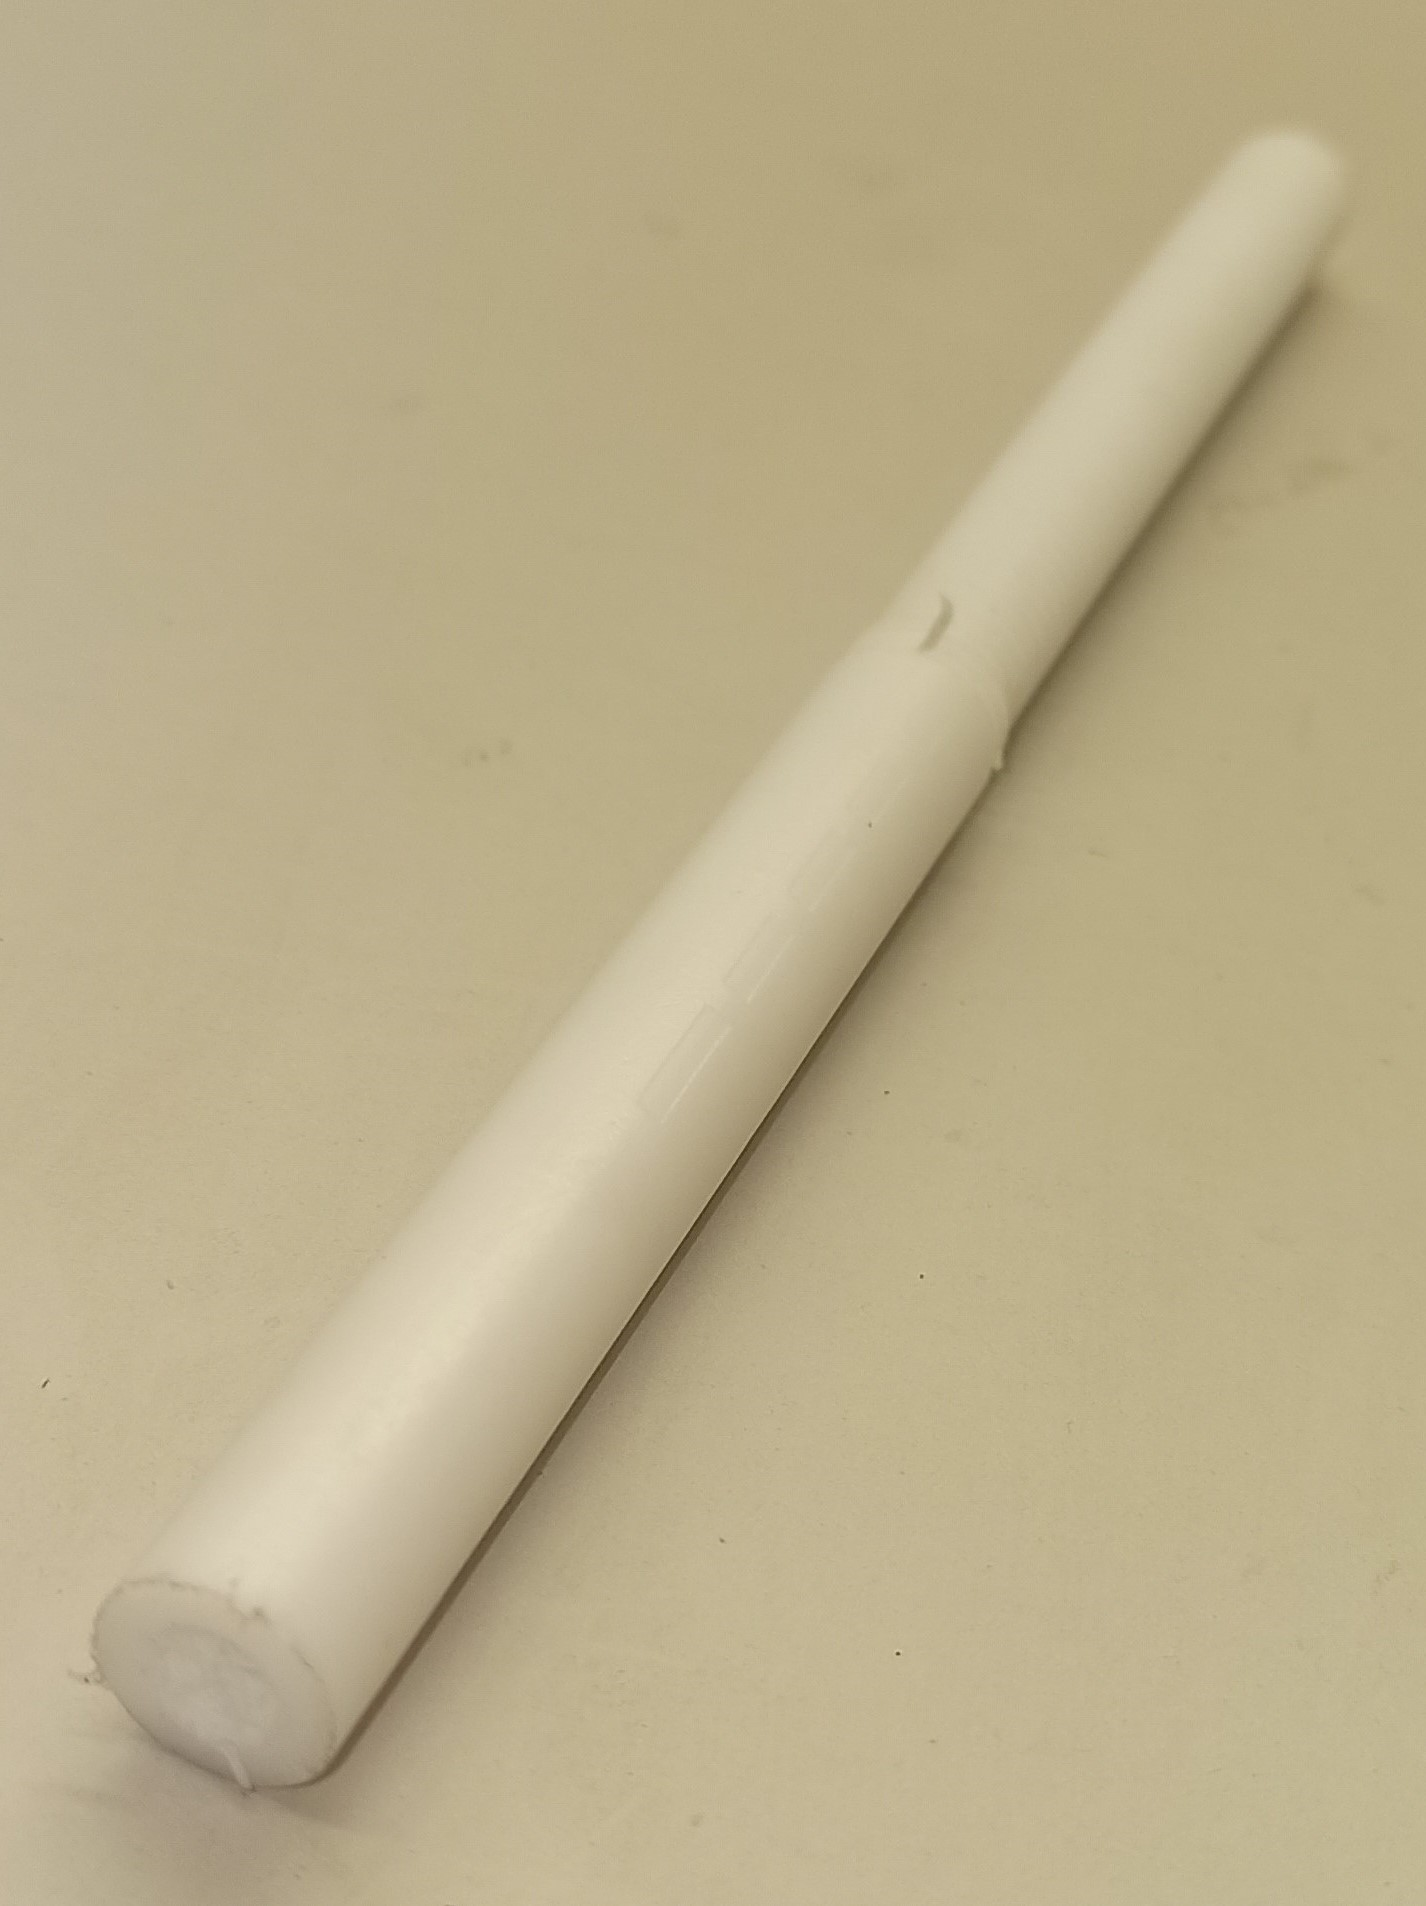
\includegraphics[width=5cm]{../ref/Abstandhalter-real.jpg}
	\label{fig:Abstandhalter-real}
	\caption{Realer Abstandhalter}
\end{figure}

Ein Abstandhalter ist ungefähr 150mm lang, das Außengewinde wird bis zur Hälfte der Teflonstange geschnitten. Der Stab wird mit dem Gewinde zuerst in die Löcher des PVC-Rohres gesteckt, damit dieser von vorne und hinten mit M10-Kunststoffmuttern an das Rohr geschraubt werden kann.

In die andere Seite des Abstandhalters wird ein Loch mit einem Durchmesser von 5mm für ein M6-Gewinde gebohrt. Mithilfe der entsprechenden Schrauben werden UV-stabilisierte Rohrschellen an dem Seitenelement montiert. Diese tolerieren Rohrdurchmesser von bis zu 18mm. Durch die Verwendung von Rohrschellen vereinfacht sich die Montage der Spirale auf ein einfaches Einschnappen des Rohres.

\begin{figure}[H]
	\begin{minipage}[b]{.4\linewidth} % [b] => Ausrichtung an \caption
		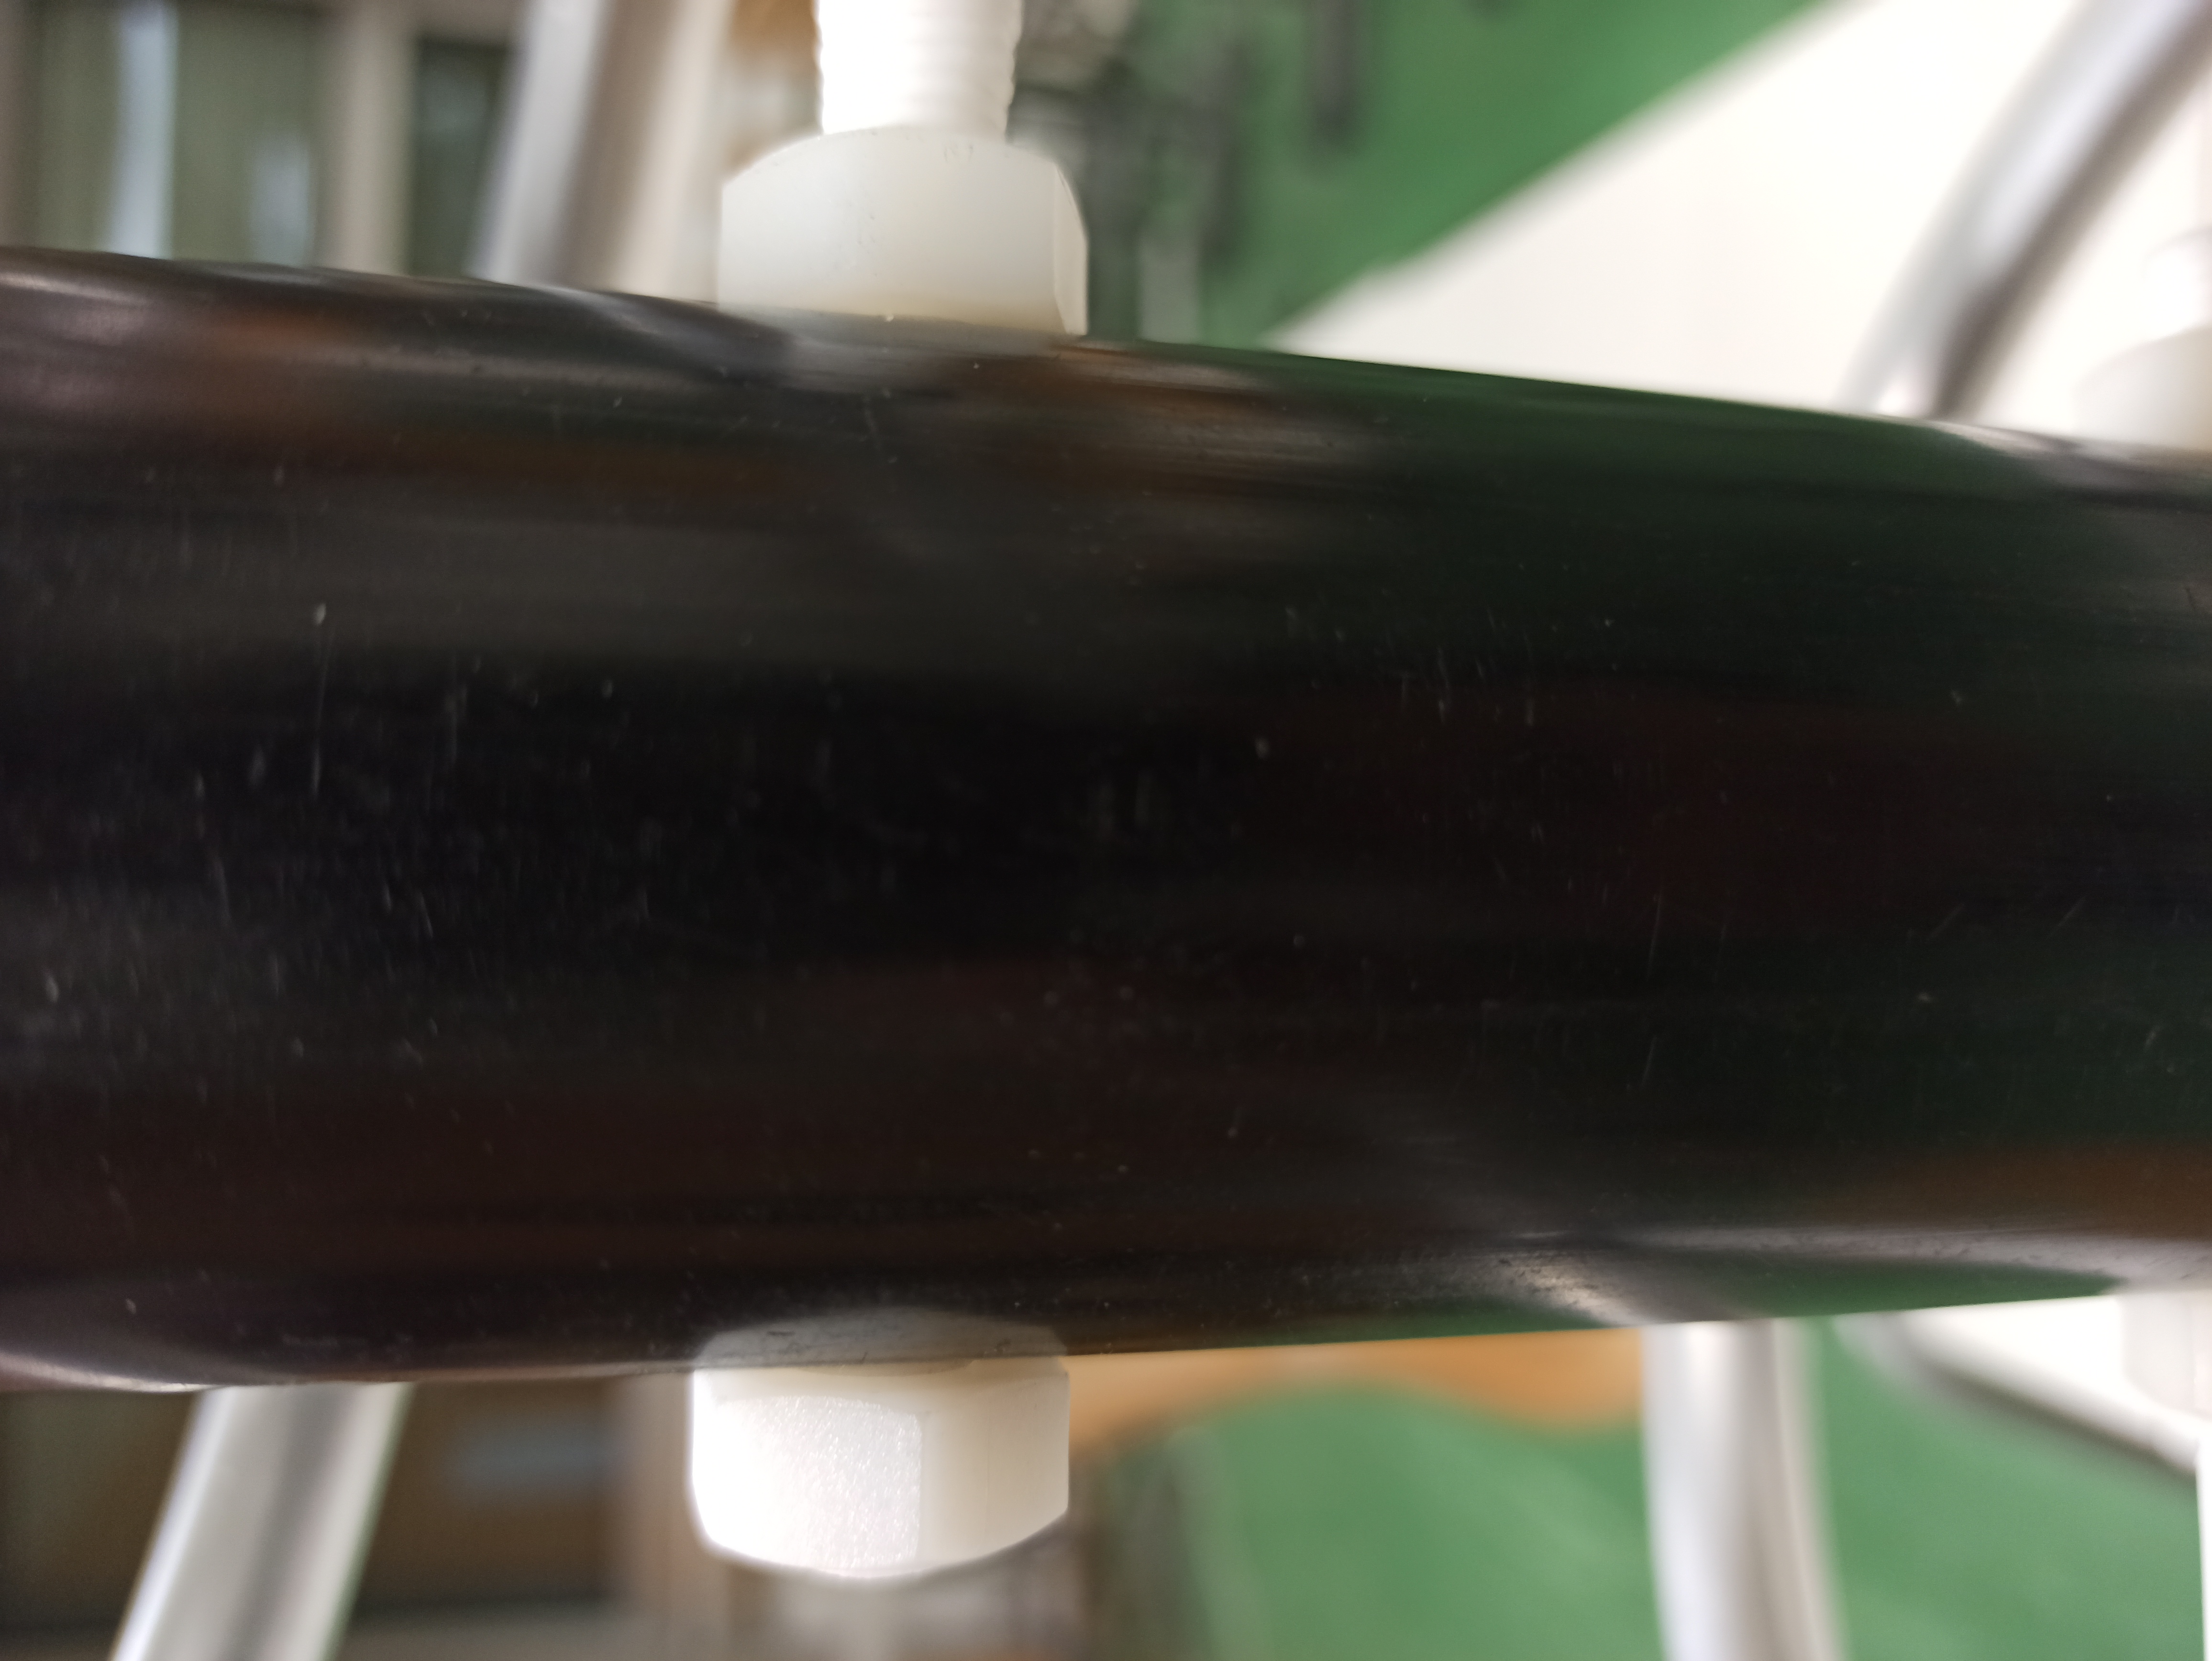
\includegraphics[width=7cm, angle=270]{../ref/Befestigung-Querelement.jpg}
		\label{fig:Abstandhalter-Befestigung}
	\end{minipage}
	\hspace{.1\linewidth}% Abstand zwischen Bilder
	\begin{minipage}[b]{.4\linewidth} % [b] => Ausrichtung an \caption
		\includegraphics[width=7cm, angle=270]{../ref/Rohrklemme-an-Spirale.jpg}
		\label{fig:Seitenelement-an-Spirale}
	\end{minipage}
	\caption{Links: Befestigung des Abstandhalters am Rohr. Rechts: Eingeschnappter Abstandhalter an der Spirale}
\end{figure}

Der Rohrflansch bildet das Bindeelement zwischen dem PVC-Rohr und der Reflektorplatte. Dieser hat einen Innendurchmesser von 51mm, und eine Wandstärke von 4mm. Es wird folglich 1mm an Toleranz geboten, damit das PVC-Rohr montiert werden kann. 

Der Rohrflansch besteht aus einem Rohr, in welches zwei durchgehende Löcher mit einem Durchmesser von 11mm gebohrt wurden, und einer Platte in die ebenfalls zwei Löcher mit einem Durchmesser von 13,5mm gebohrt wurden. Die Platte und das Rohr werden aneinander geschweißt. Das resultierende Bauteil bildet das Bindeglied zwischen Reflektor und PVC-Rohr.

Für den Reflektor wurde eine runde Aluminiumplatte gewählt. Für die reale Konstruktion wurden Löcher in den äußeren Rand der Platte gelasert, um den Luftwiderstand zu reduzieren. Um eventuelle Störungen durch spezifische Maße wie beispielsweise $\frac{\lambda}{4}$ zu vermeiden, wurden die Löcher um einiges kleiner als dieses Maß dimensioniert.

\begin{figure}[H]
	\begin{minipage}[b]{.4\linewidth} % [b] => Ausrichtung an \caption
		\includegraphics[angle=270,width=\linewidth]{../ref/Rohrflansch-Antenne.jpg}
		\label{fig:Rohrflansch-Antenne-Verbindung}
	\end{minipage}
	\hspace{.1\linewidth}% Abstand zwischen Bilder
	\begin{minipage}[b]{.4\linewidth} % [b] => Ausrichtung an \caption
		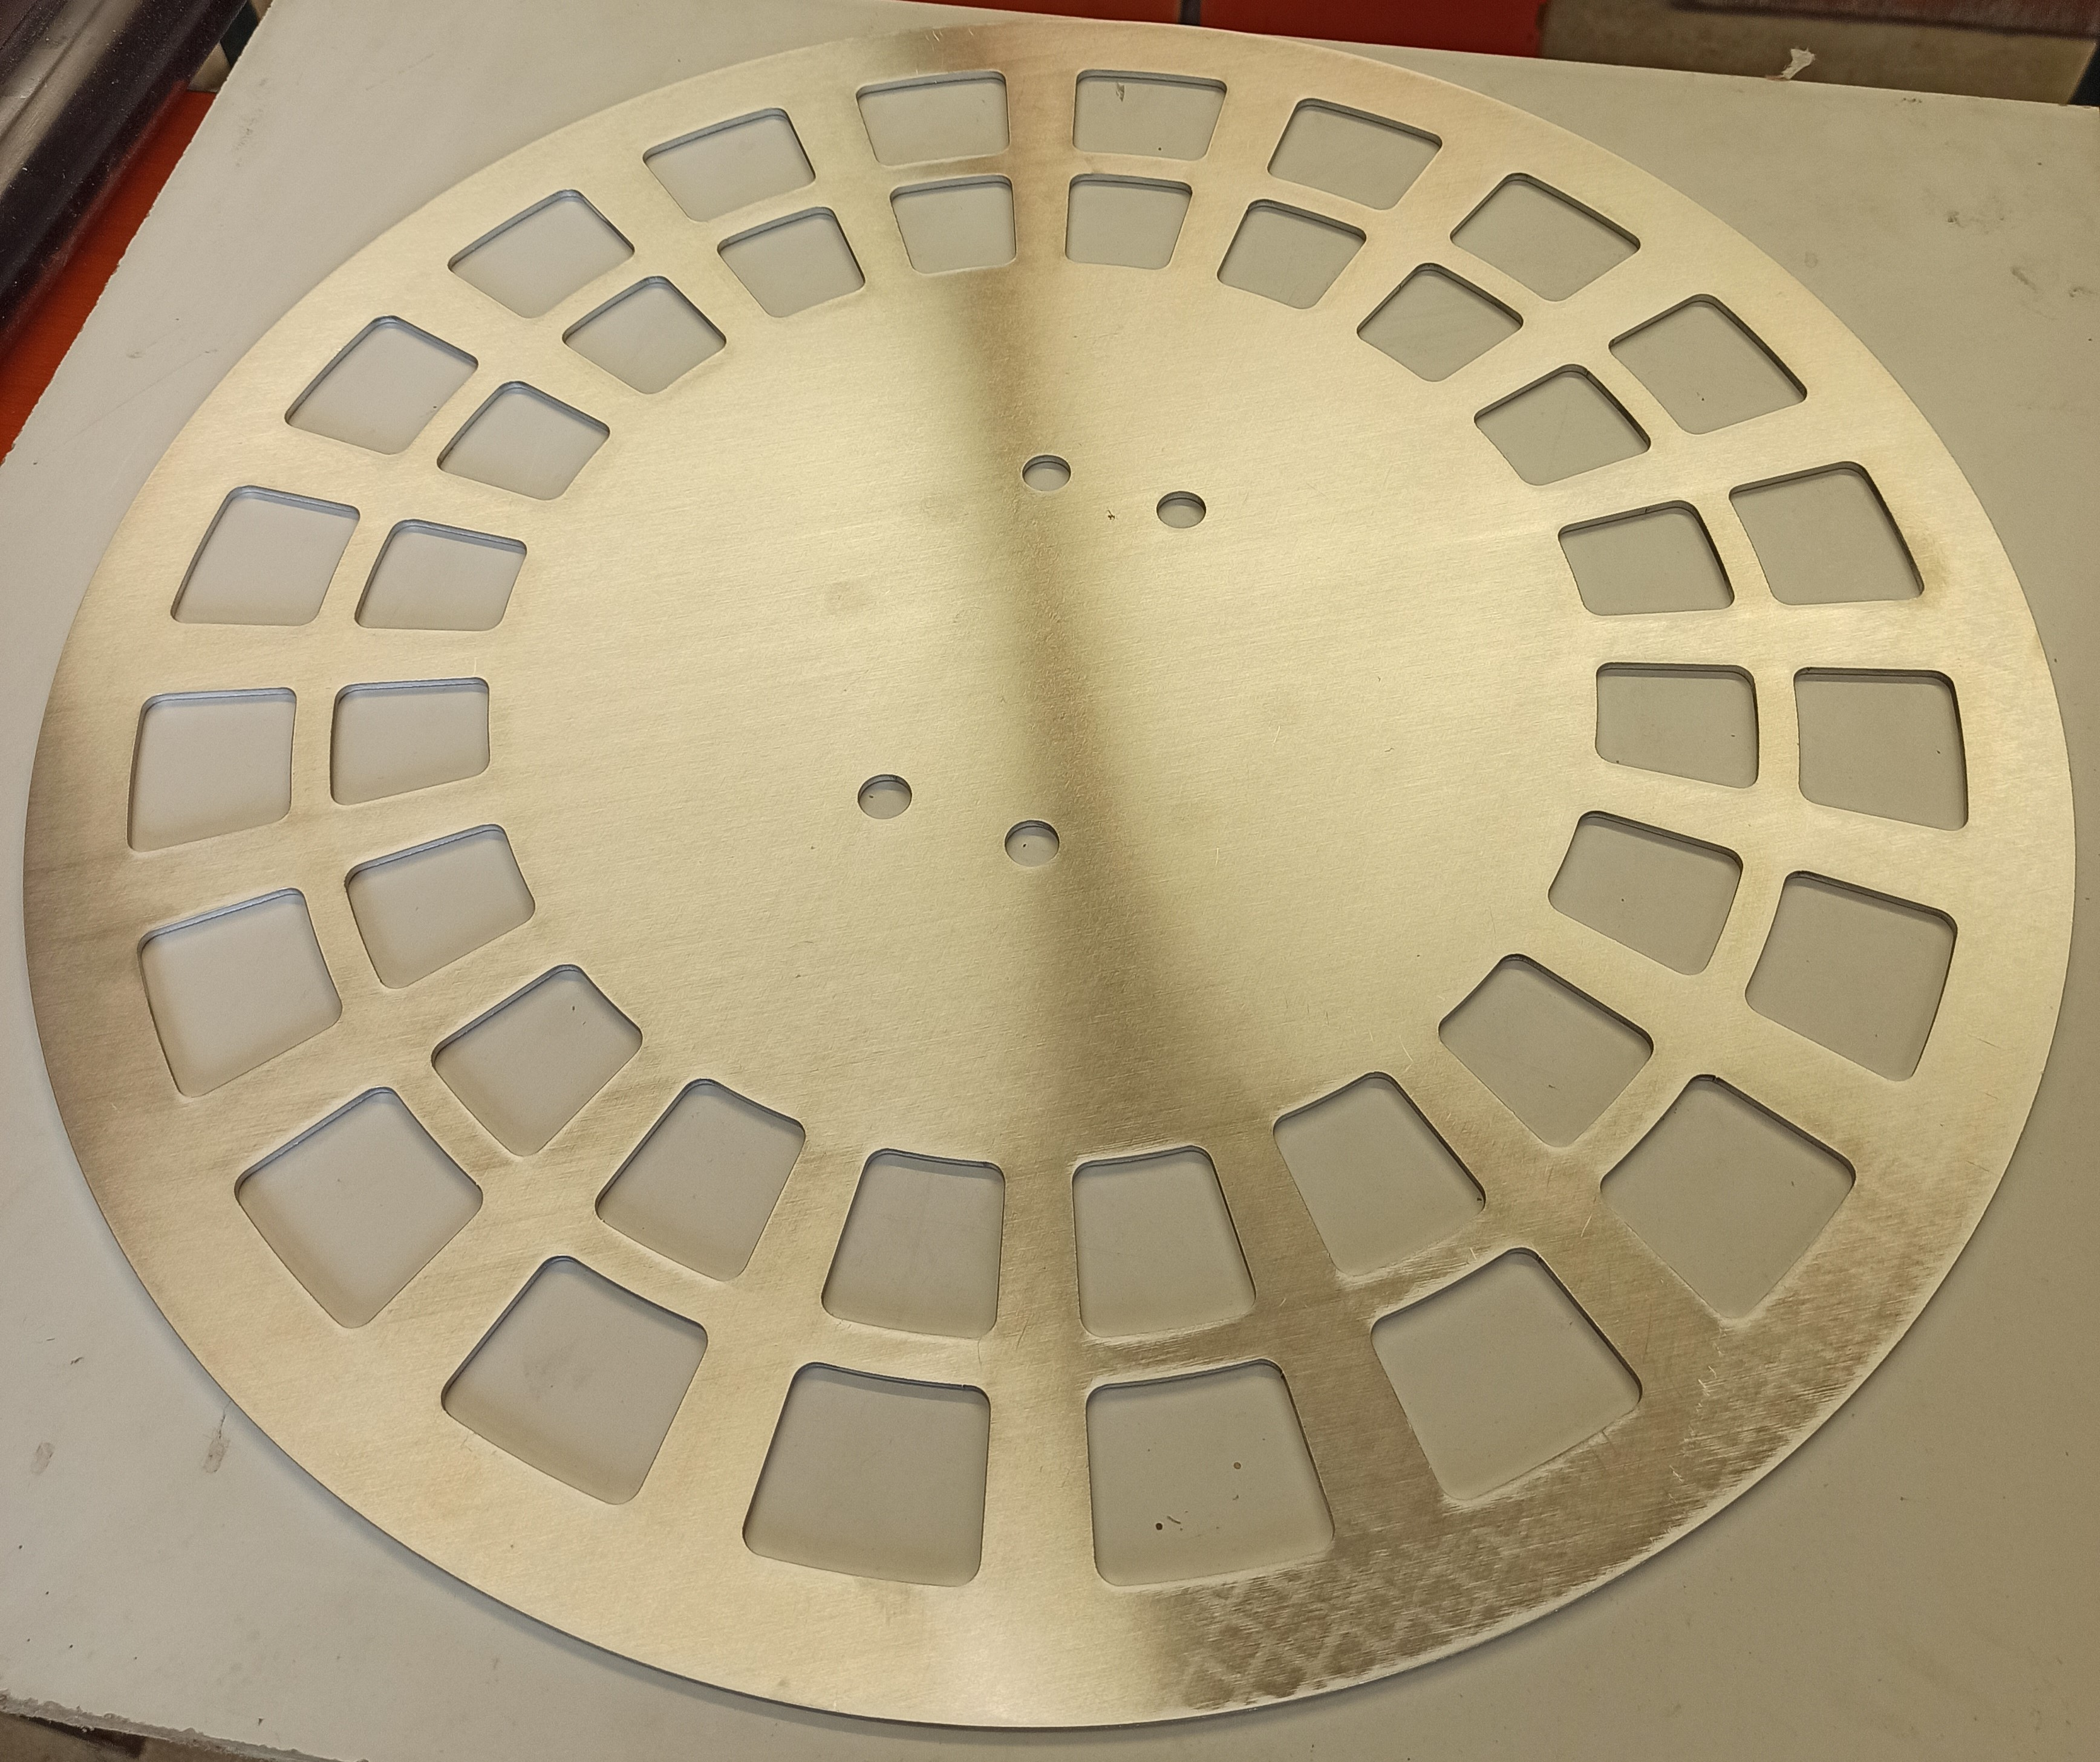
\includegraphics[width=\linewidth]{../ref/Reflektor.jpg}
		\label{fig:Reflektor}
	\end{minipage}
	\caption{Reflektor (rechts) im Vergleich mit dem daran befestigten Rohrflansch (links)}
\end{figure}

In der Mitte des Reflektors werden vier Löcher mit einem Durchmesser von 13,5mm gebohrt an denen der Rohrflansch befestigt wird. 

Die Helix wurde mit denselben Maßen gefertigt, welche in der Simulation ermittelt wurden. Hierfür wurde ein Aluminiumrohr verwendet, welches zu einer Spirale gebogen wurden die einen Durchmesser von 270mm, eine Höhe von ca. 1039,2mm und konsequent eine Steigung von 11,5° beziehungsweise einen Abstand zwischen den Windungen von 173,2mm ($\frac{\lambda}{4}$) hat.

\begin{figure}[h!]
	\centering
	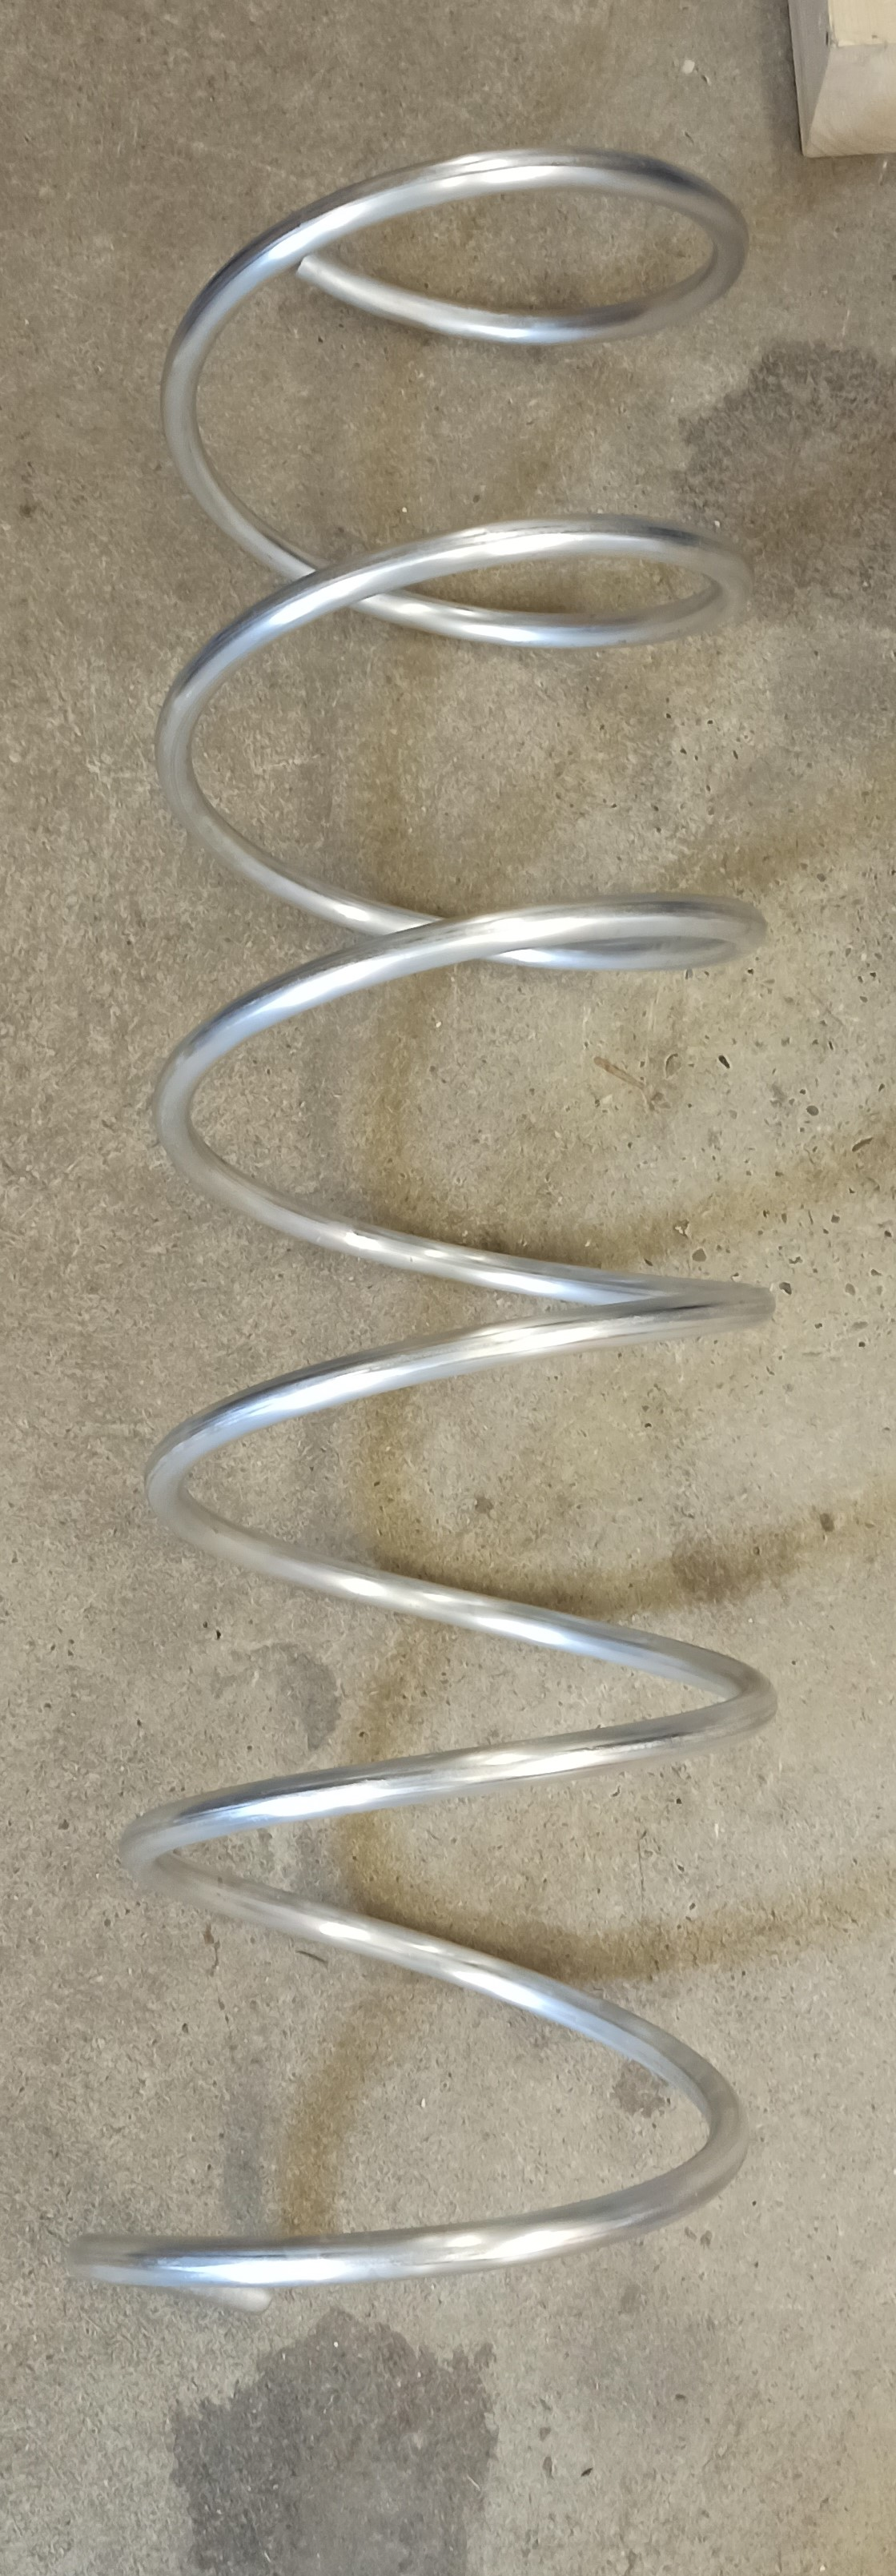
\includegraphics[width=5cm,angle=90]{../ref/Spirale.jpg}
	\caption{Die Spirale}
	\label{fig:Spirale}
\end{figure}

Um die Helixantenne wasserdicht zu machen wurden kurz abgeschnittene Aluminium-Rundlinge auf die Öffnungen der Spirale geschweißt. Am unteren Ende der Helix, an der der Innenleiter des Koaxialkabels befestigt wird, wurde ein Gewinde in den Aluminium-Rundling geschnitten.

\begin{figure}[h!]
	\begin{minipage}[b]{.4\linewidth} % [b] => Ausrichtung an \caption
		\includegraphics[width=\linewidth]{../ref/Deckel-oben.jpg}
		\label{fig:Deckel-Helix-Oben}
	\end{minipage}
	\hspace{.1\linewidth}% Abstand zwischen Bilder
	\begin{minipage}[b]{.4\linewidth} % [b] => Ausrichtung an \caption
		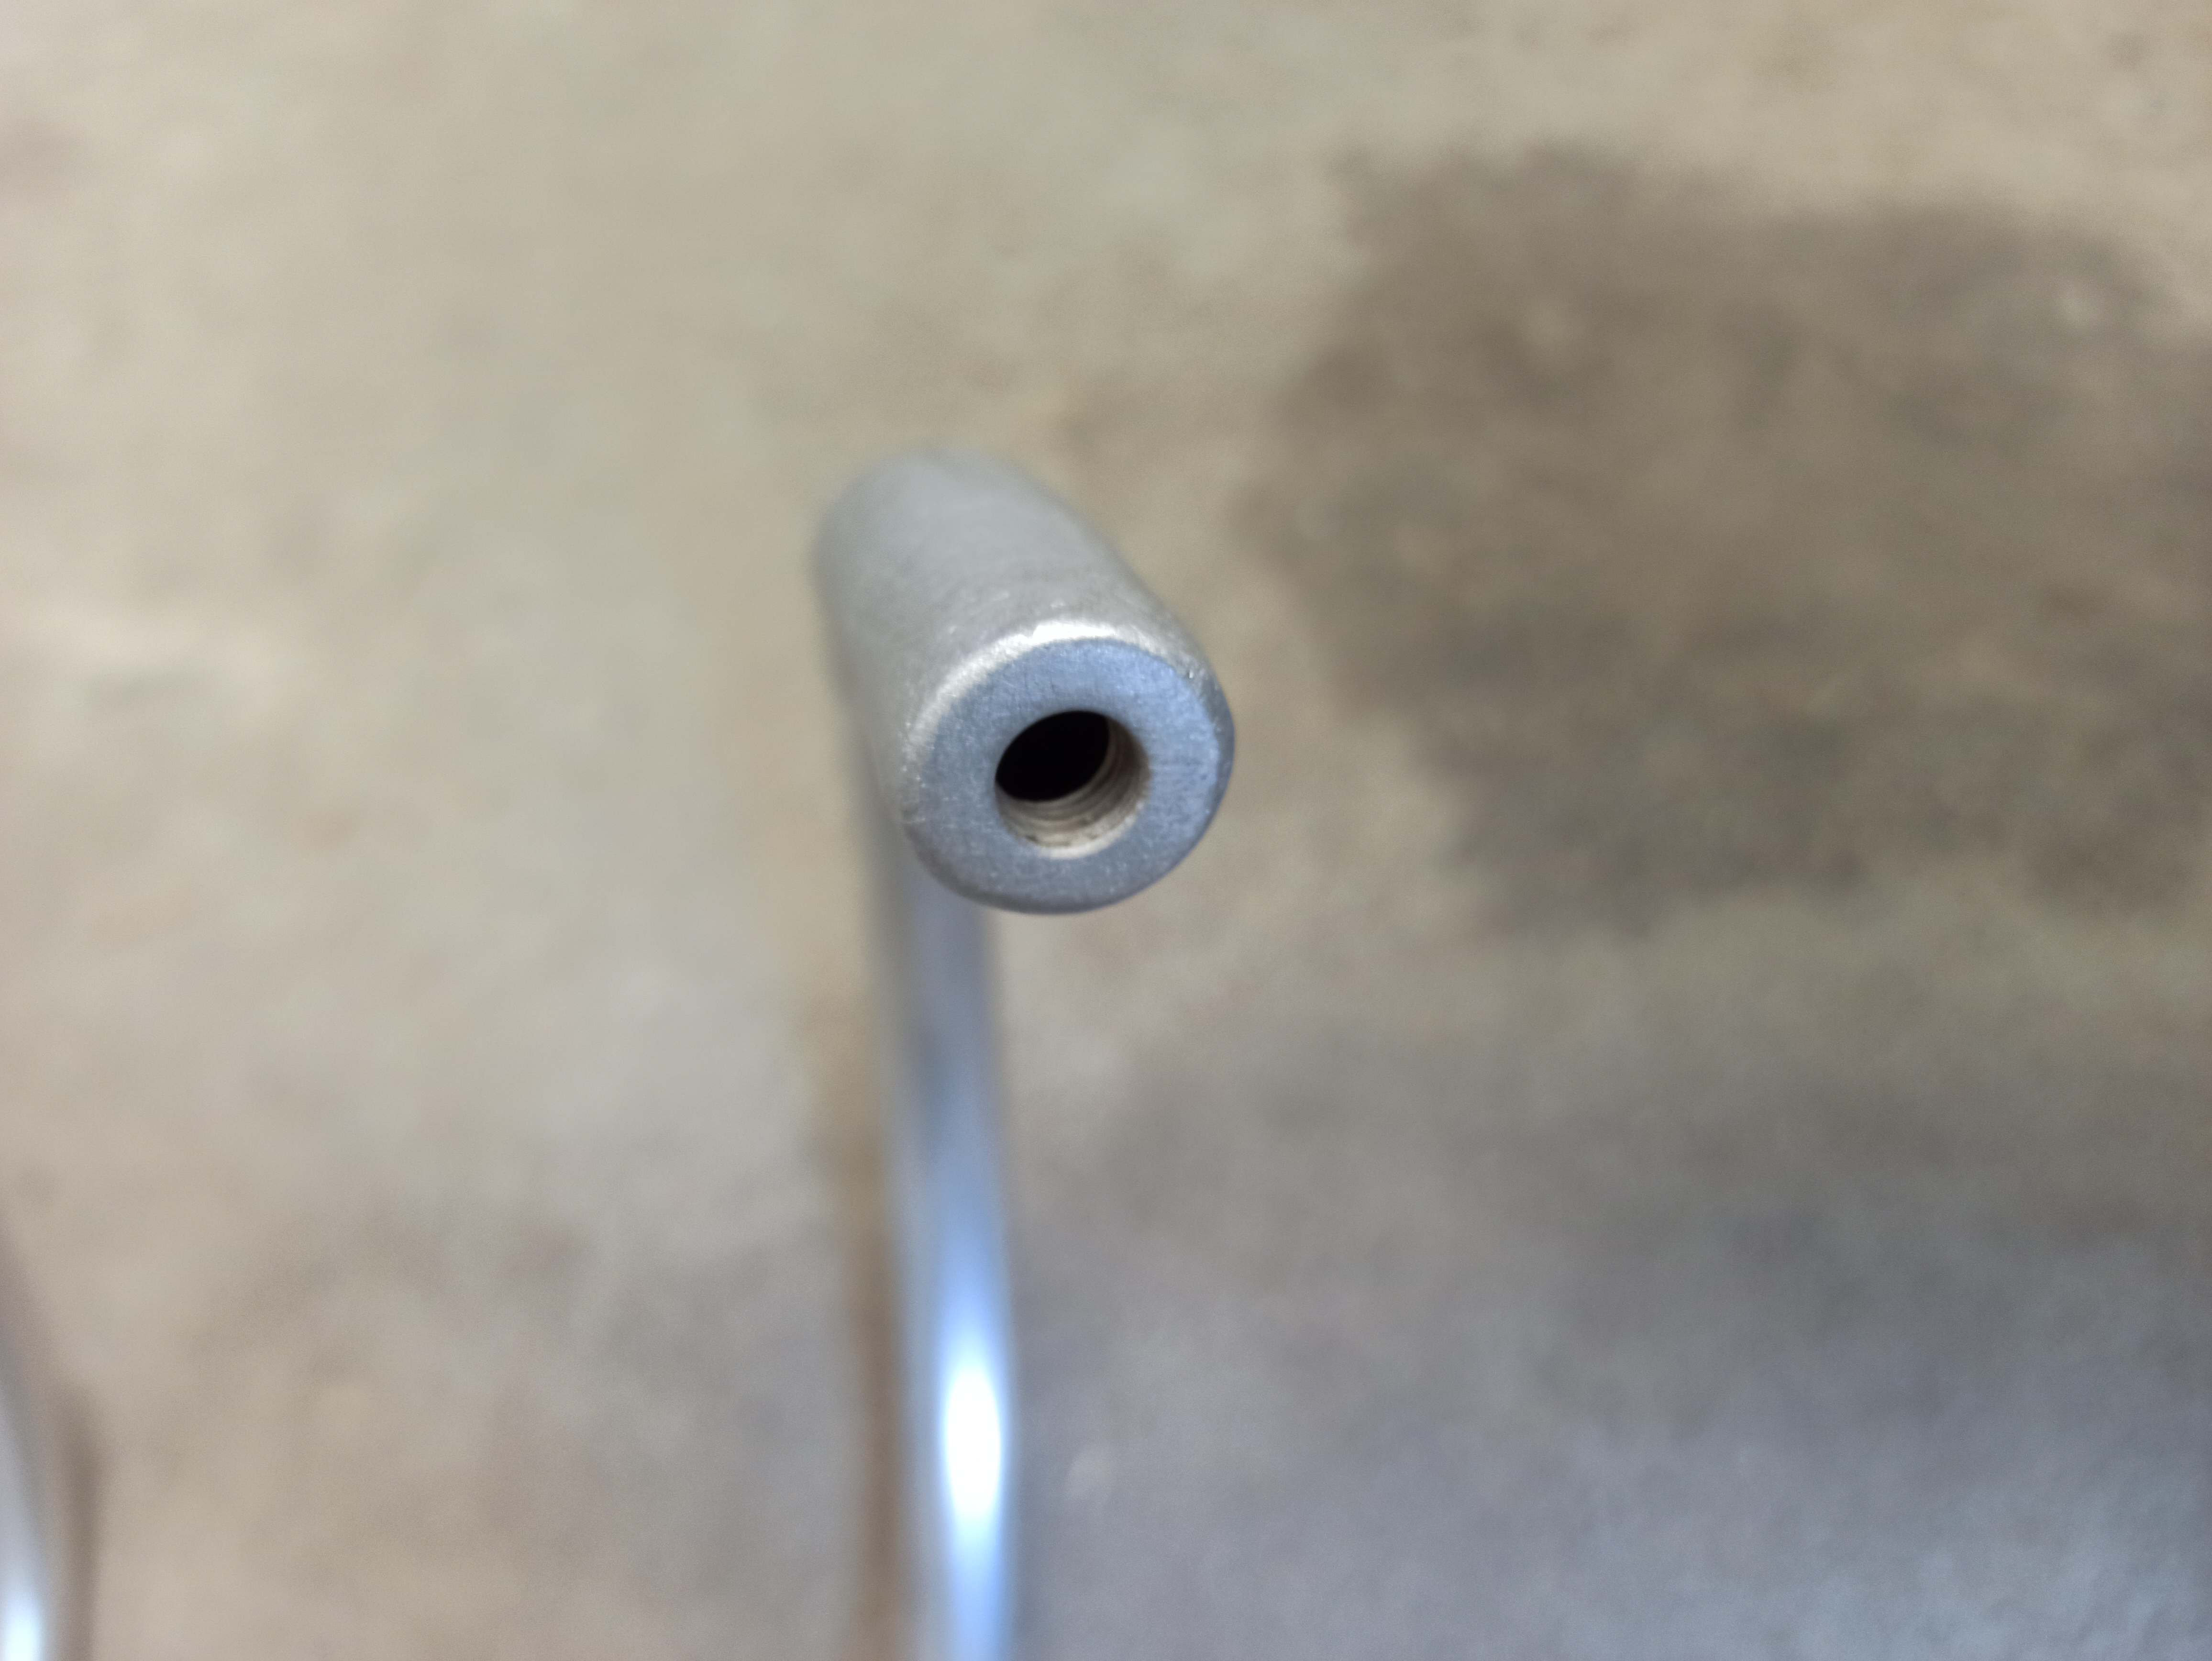
\includegraphics[width=\linewidth]{../ref/Anschluss-unten.jpg}
		\label{fig:Deckel-Helix-Unten}
	\end{minipage}
	\caption{Links: Zugeschweißtes oberes Ende der Helix.Rechts: Gewinde am unteren Ende der Helix zur Anbringung des Innenleiters}
\end{figure}

Mithilfe dieses Gewindes kann ein Kabel durch eine Schraube montiert, und am Innenleiter der BNC-Buchse angelötet werden.

Um die PVC-Rohre vor Wasser zu schützen wurden Abdeckungen 3D-gedruckt. Durch die Verwendung eines speziellen Filaments vom Typ DuraPro ASA, ist das Resultat eine UV-resistente Rohrabdeckung. Durch diese Eigenschaft eignet sich dieses Filament exzellent für den Einsatz im Freien.

\begin{figure}[H]
	\centering
	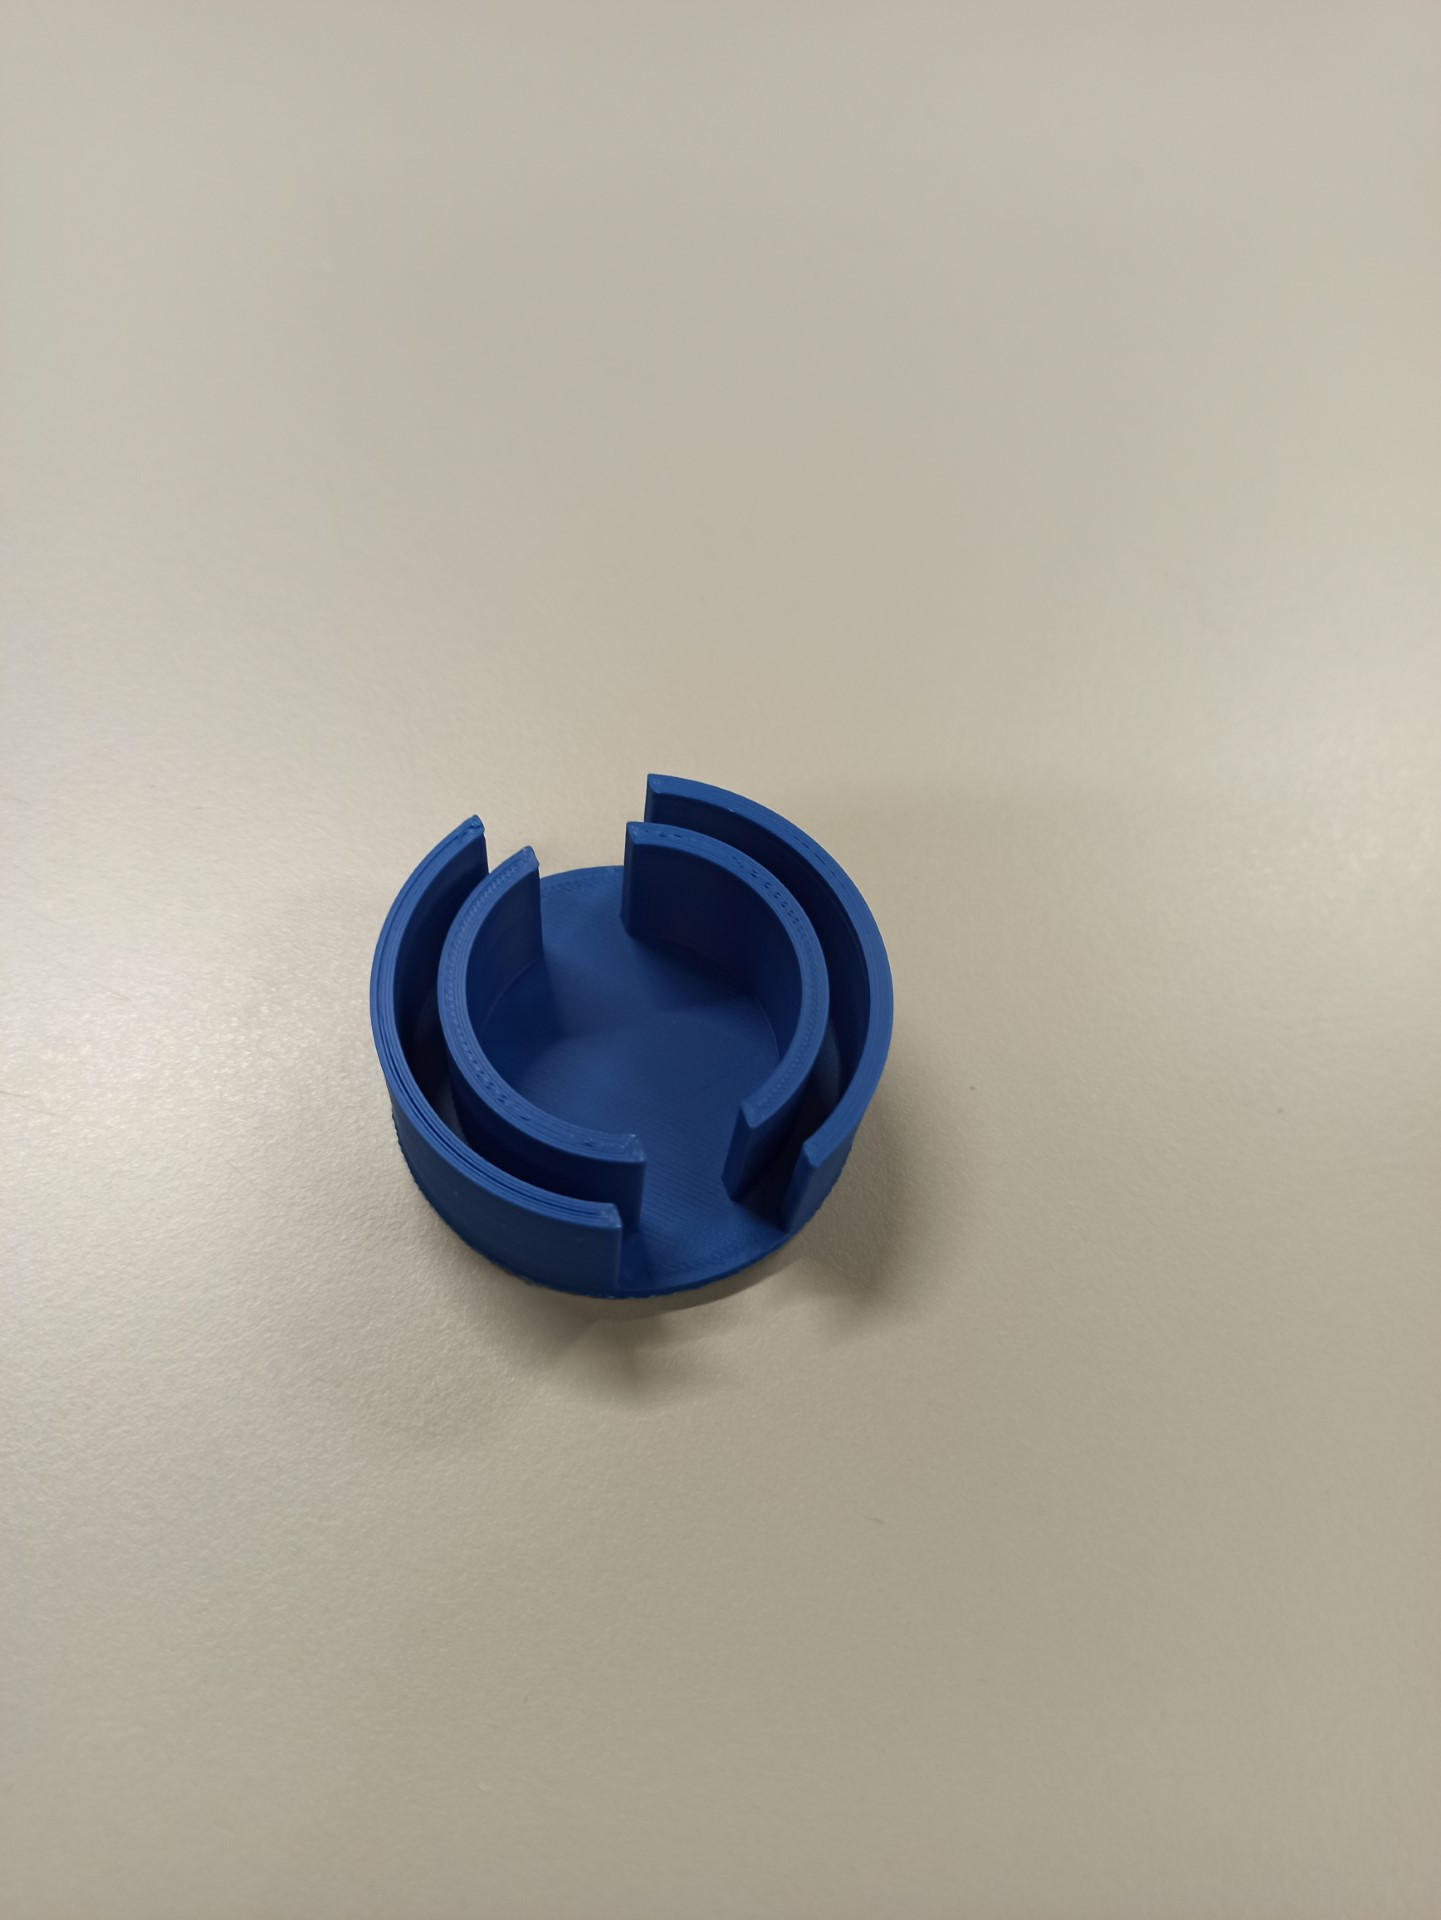
\includegraphics[width=5cm]{../ref/Abdeckung-PVC-Rohr.jpg}
	\caption{Die Abdeckung des PVC-Rohres}
	\label{fig:PVC-Rohr-Abdeckung}
\end{figure}

Die BNC-Buchse befindet sich direkt unter dem Ende der Spirale. Der Innenleiter wird, wie bereits erwähnt, an der Helix befestigt. Der Außenleiter wird mit dem Reflektor verschraubt.

\begin{figure}[H]
	\begin{minipage}[b]{.4\linewidth} % [b] => Ausrichtung an \caption
		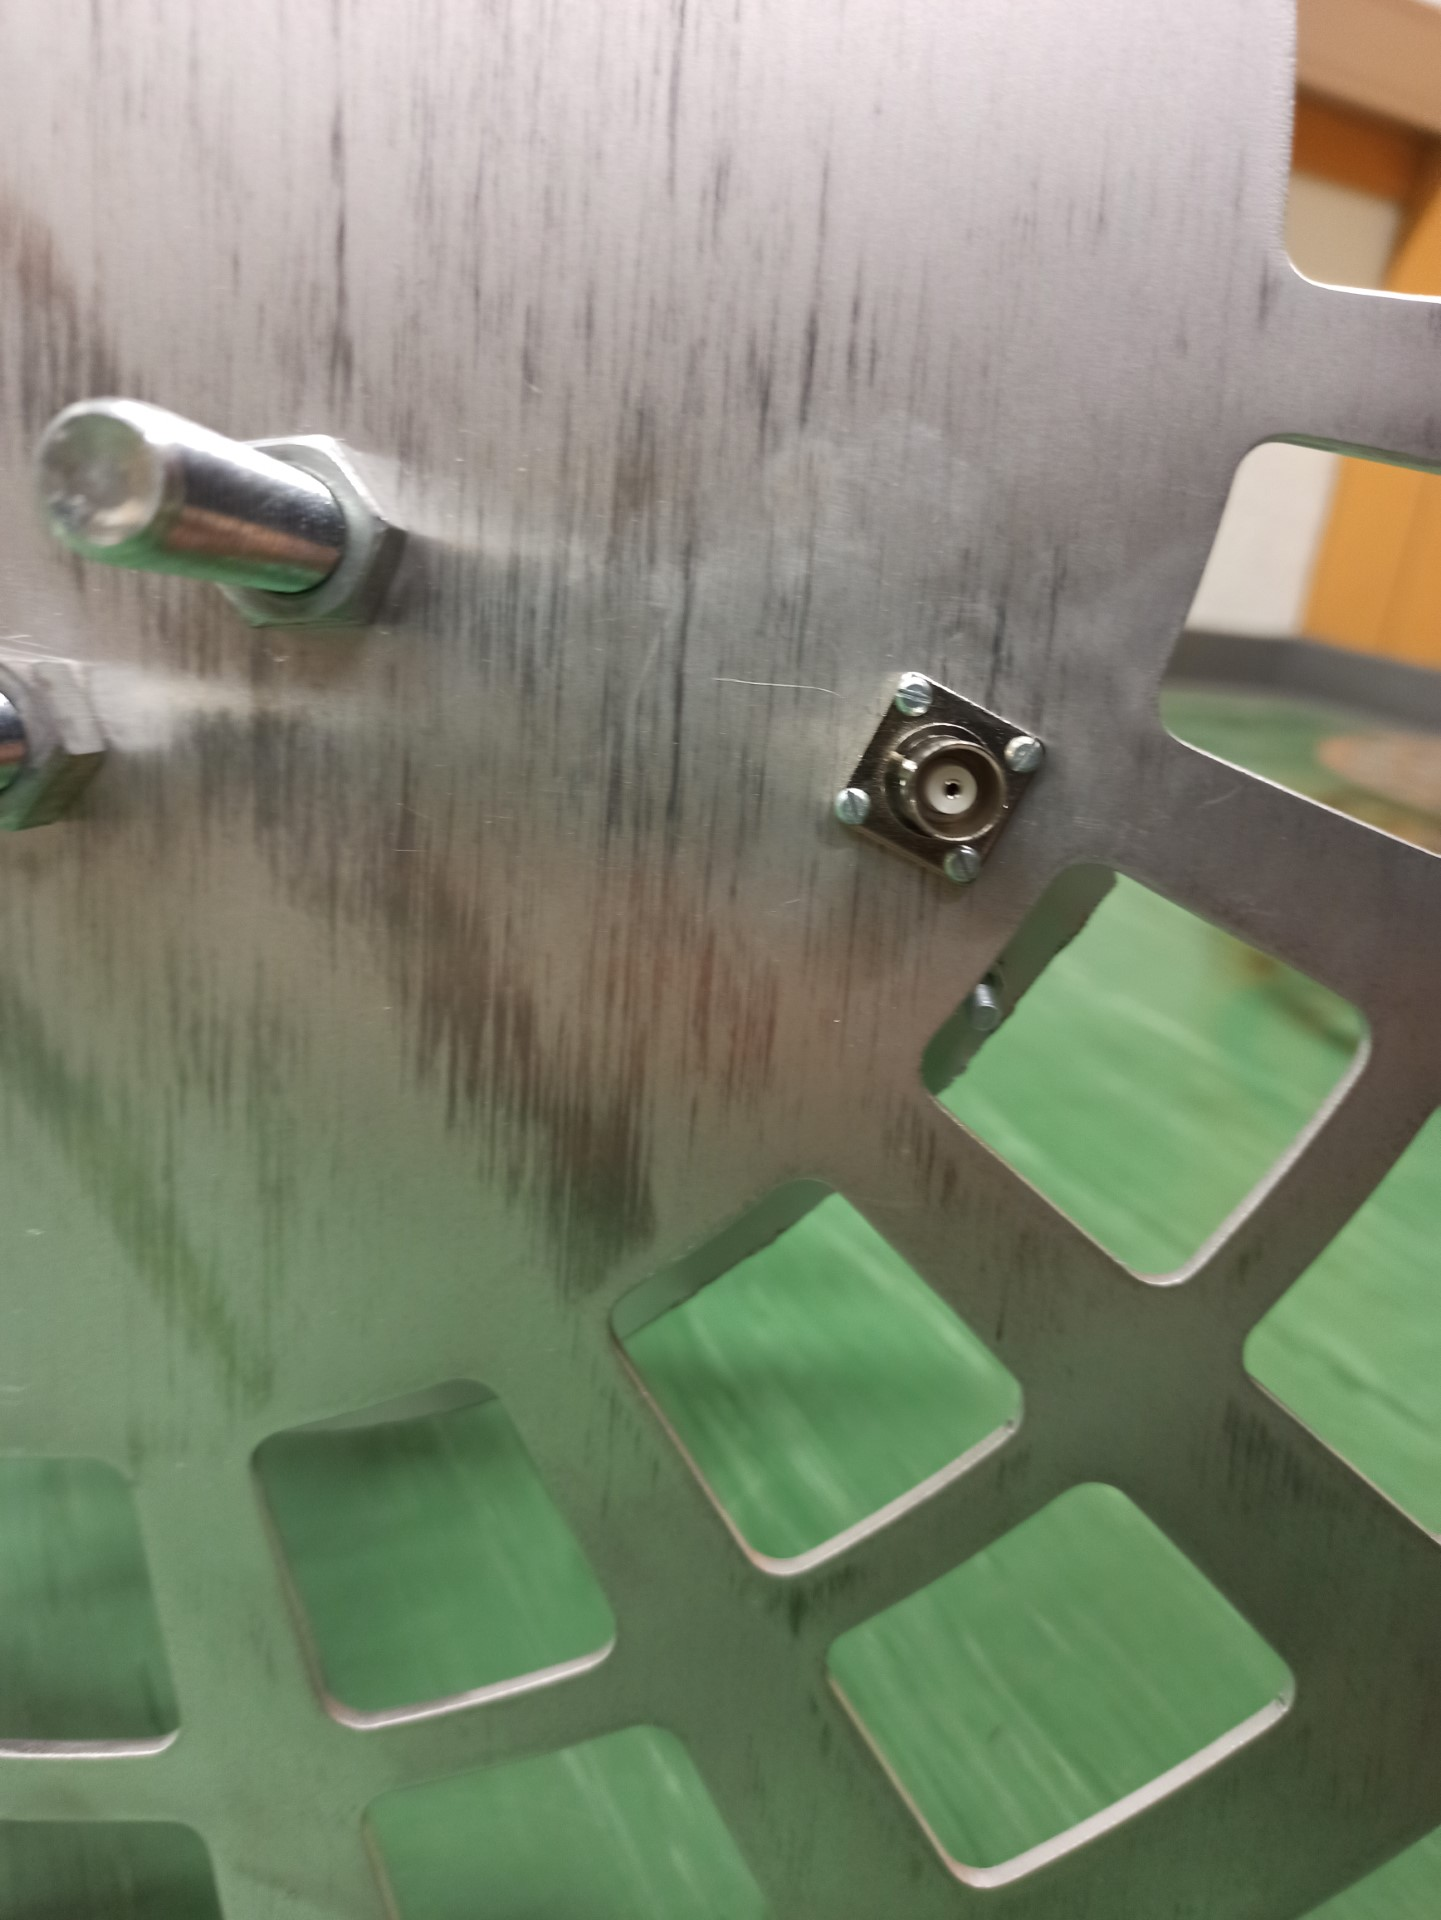
\includegraphics[width=\linewidth]{../ref/BNC-Buchse.jpg}
		\label{fig:BNC-Buchse}
	\end{minipage}
	\hspace{.1\linewidth}% Abstand zwischen Bilder
	\begin{minipage}[b]{.4\linewidth} % [b] => Ausrichtung an \caption
		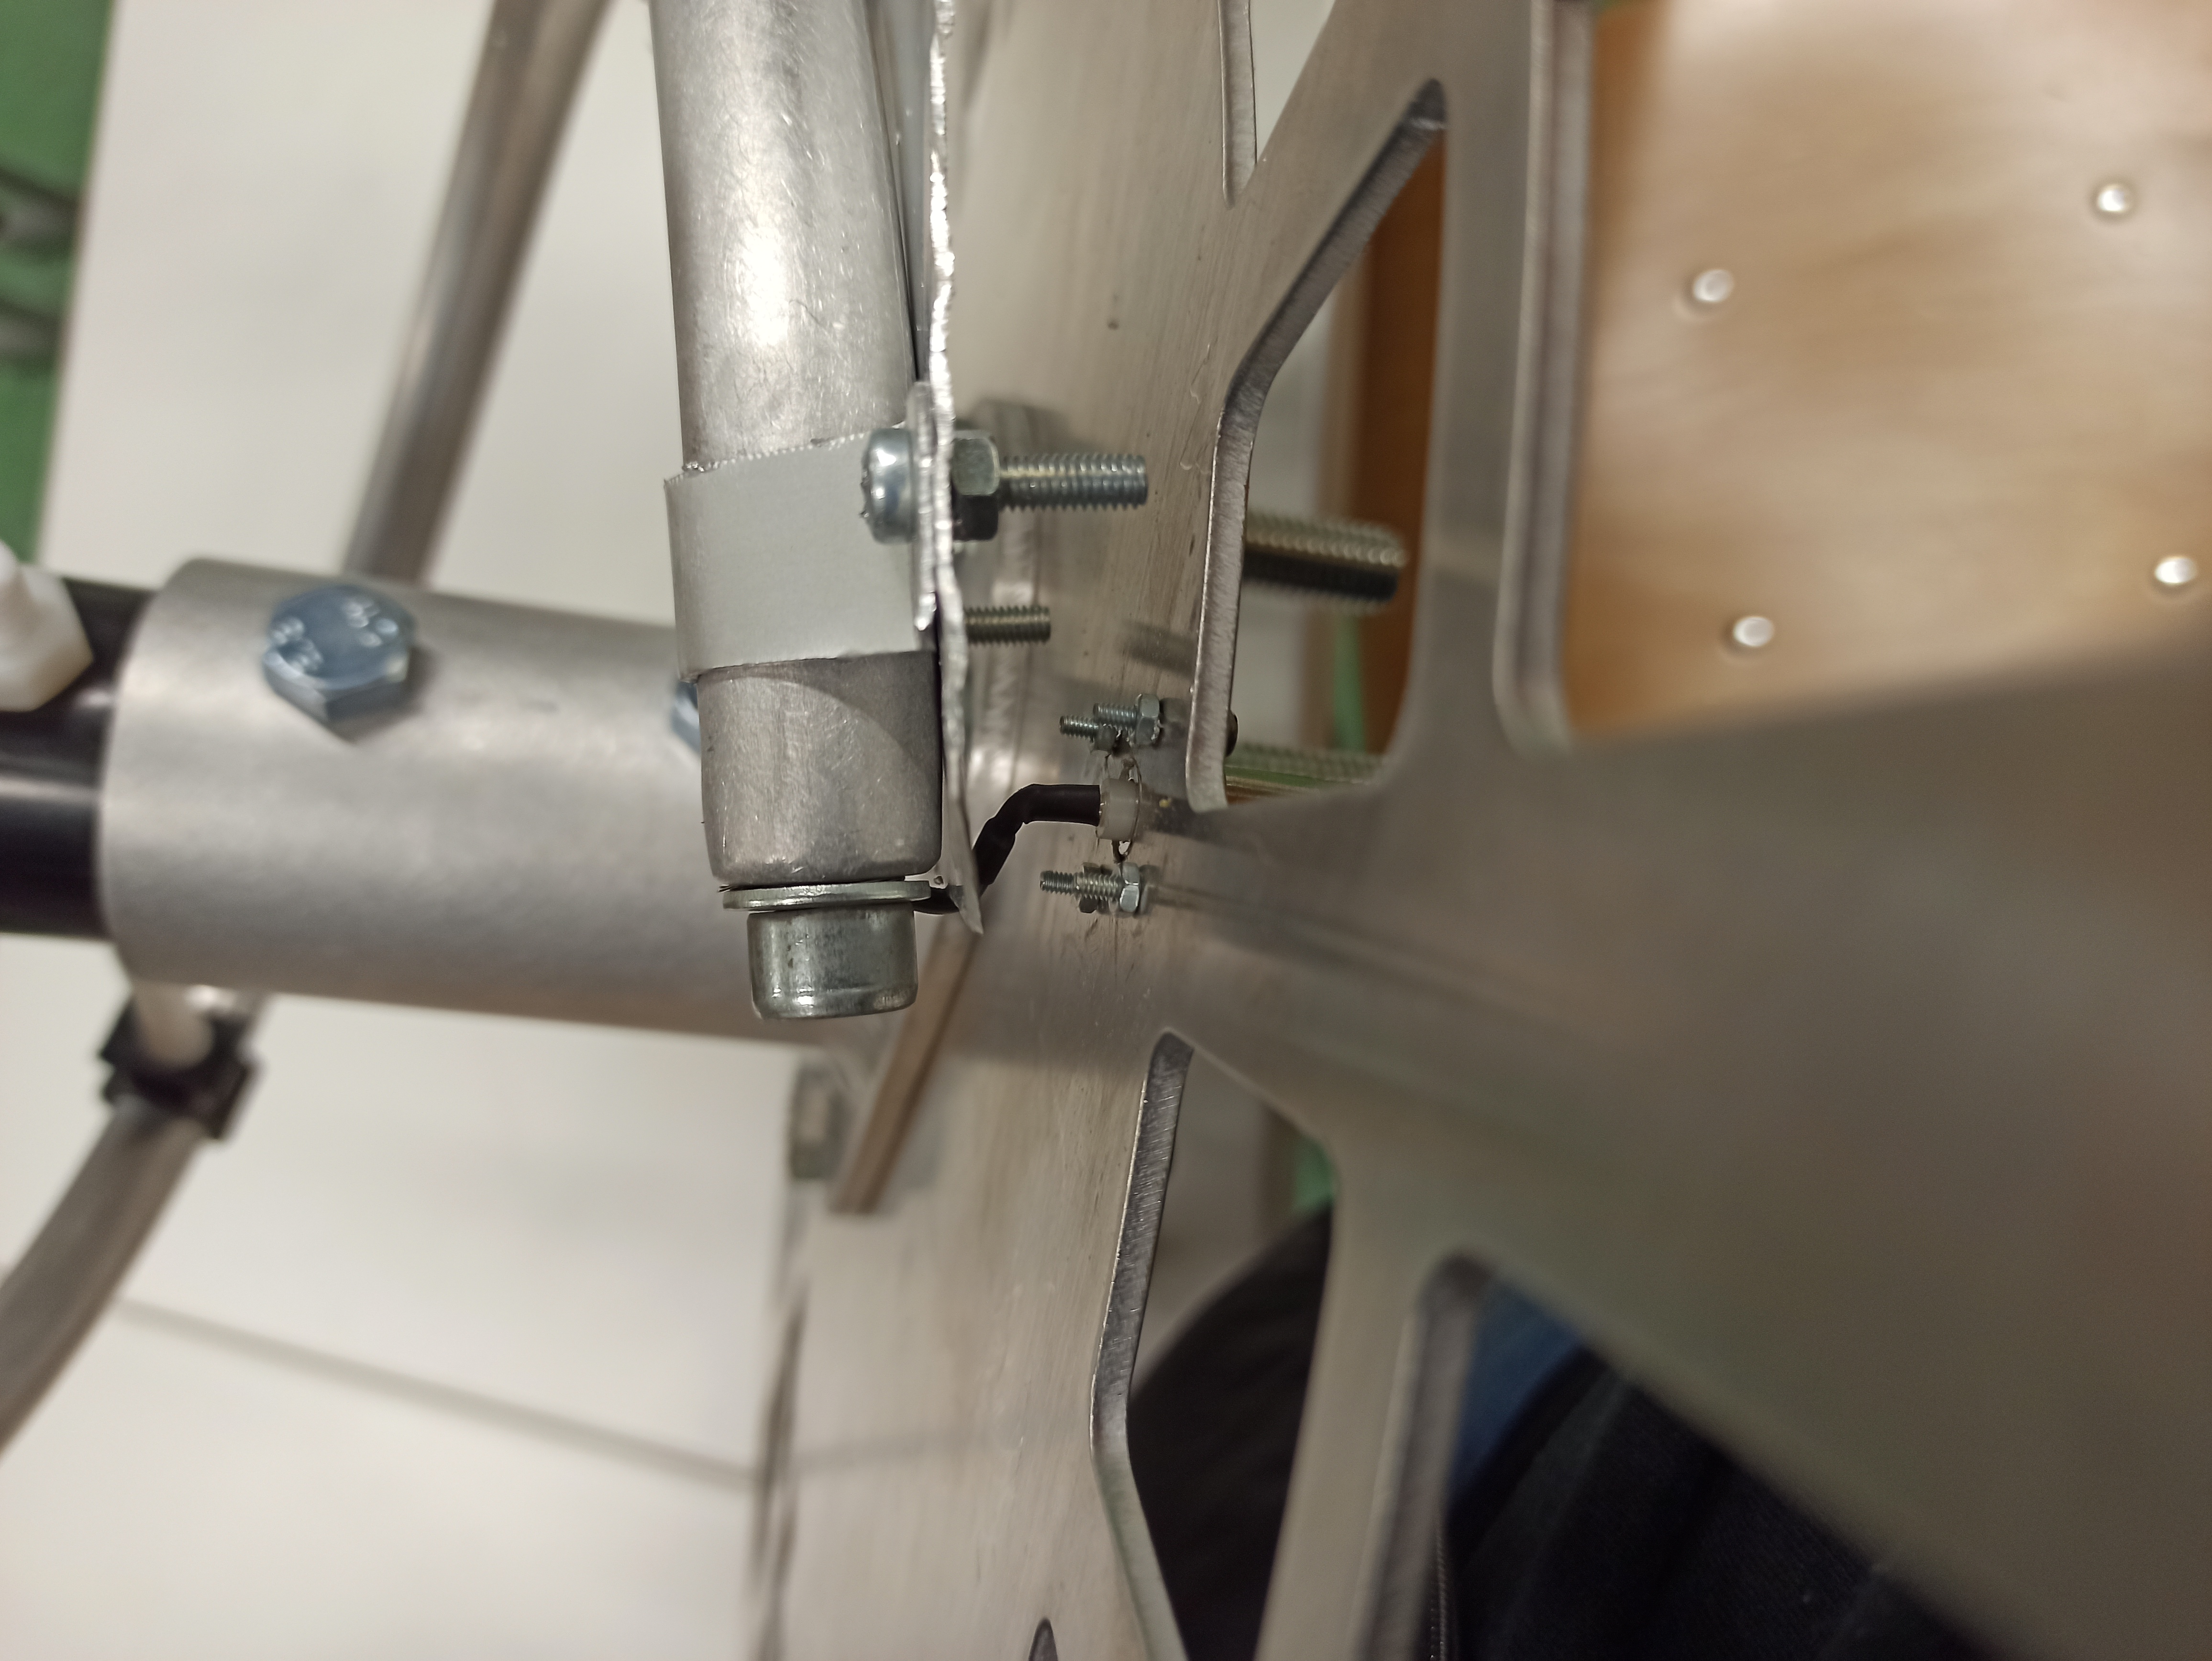
\includegraphics[angle=270,width=\linewidth]{../ref/Befestigung-Innenleiter.jpg}
		\label{fig:Innenleiter-Befestigung}
	\end{minipage}
	\caption{Koaxialkabel-Anschluss}
\end{figure}

\section{Anpassung}
Um eine einzelne Helixantenne anzupassen gibt es verschiedene Möglichkeiten. Eine weit verbreitete Option ist es, einen entsprechend dimensionierten Blechstreifen mit einer Länge von $\frac{\lambda}{4}$ entlang des unteren Endes der Helix zu montieren. Dieser agiert als Resonanztransformator und soll die Impedanz der Antenne auf einen Wert von 50$\Omega$ senken \cite{kgwadi_parametric_2014}.

\begin{figure}[H]
	\centering
	\includegraphics[width=7cm]{../ref/Anpassstreifen.jpg}
	\caption{Der realisierte Blechstreifen für die Impedanzanpassung}
	\label{fig:matching-strip}
\end{figure}

Die Breite des Blechstreifens wurde empirisch ermittelt und wurde mit 6cm festgelegt. Um den S11-Parameter auf einen akzeptablen Wert zu bringen, wird der Abstand zwischen Reflektor und Spirale verringert. Dadurch beeinflussen sich der Blechstreifen und die auf Masse liegende Reflektorplatte auf eine Weise, die die Performance der Antenne steigert.

\section{Erweiterung der Helixantenne als Array}
Nun wird die Helixantenne durch drei weitere identische Helixantennen erweitert, welche zusammen ein Array bilden. Hierbei ist der Abstand zwischen den einzelnen Antennen von Relevanz um den Gesamtgewinn zu maximieren.
Der Antennengewinn eines Antennenarrays bestehend aus vier identischen Helixantennen liegt in der Theorie bei dem vierfachen Antennengewinn einer einzelnen Wendelantenne, bzw. einer Helixantenne mit der vierfachen Windungszahl, also $4*6=24$ \cite[p. 319]{Kraus-2002-AntennasB}.

\begin{figure}[h!]
	\centering
	\includegraphics[angle=270,width=5cm]{../ref/Antennenarray2.jpg}
	\caption{Das fertige Helixantennen-Array}
	\label{fig:helixantennen-array}
\end{figure}

Hierfür muss ein Gerüst designt und aufgebaut werden, welches vier solcher Antennen halten kann, sowie die neu entstehende Impedanz der Zusammenschaltung dieser Antenne angepasst werden. Anschließend müssen Tests durchgeführt werden, die den verbesserten Antennengewinn der Antenne belegen.

\subsection{Gerüst}
\label{subsec:helix_geruest}
\begin{table}
	\begin{tabular}{|c|c|c|c|}
	\hline
	Nr. & Typ & Maße & Menge \\
	\hline
	1 & Aluminiumrohr & \O42x2,5mm 0,77m & 1x \\
	\hline
	2 & Aluminium-Vierkantrohr & 60x100x3mm 0,9m & 2x \\
	\hline
	3 & Rohrflansch (Struktur) & \O innen 45mm & 2x\\
	\hline
	4 & Zylinderkopfschraube & \O M12x80mm & 4x\\
	\hline
	5 & Sechskantschraube & \O M10x20mm & 24x\\
	\hline
	6 & Linsenkopfschraube & \O M5x10mm & 16x\\
	\hline
\end{tabular}
\caption{Stückliste Gerüst}
\end{table}

Als Gerüst wurde die Form eines $"$H$"$ gewählt. Hierdurch liegt der Massenmittelpunkt der Gesamtkonstruktion nur knapp über dem Mittelpunkt des Rotors, was das zur Rotation benötigte Moment verringert. Um dies zu beweisen lässt sich die Formel für das mechanische Moment betrachten.
\begin{equation}
	M=F*r*\sin(\alpha)
	\label{form:drehmoment}
\end{equation}
Hierbei ist r die Länge des Hebels, und in diesem Kontext der Abstand des Schwerpunktes der Konstruktion zum Mittelpunkt. Je näher der Schwerpunkt am Mittelpunkt ist, desto weniger Moment wird benötigt, um die Konstruktion zu bewegen. Dies lässt sich mit einer Grafik visualisieren.

\begin{figure}[h!]
	\centering
	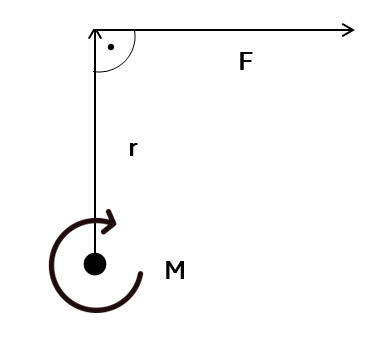
\includegraphics[width=7cm]{../ref/Drehmoment.png}
	\caption{Das Drehmoment visualisiert}
	\label{fig:mechanische-moment}
\end{figure}

Um das mechanische Drehmoment in beliebigen Lagen zu berechnen werden einige zusätzliche Informationen benötigt, wie die Masse und der Massenmittelpunkt der Konstruktion.

\begin{figure}[h!]
	\centering
	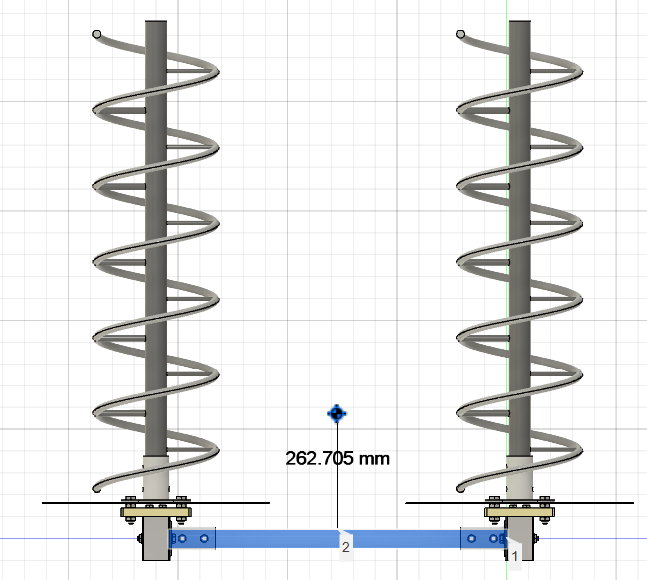
\includegraphics[width=7cm]{../ref/Massenmittelpunkt.png}
	\caption{Das Massenzentrum der Konstruktion}
	\label{fig:massenmittelpunkt}
\end{figure}

Es ist ersichtlich, dass sich der Massenmittelpunkt 262,705mm über dem oberen Ende des Strukturrohres befindet. Um daraus folgt, dass der Massenmittelpunkt $\frac{42mm}{2}+262,705mm=283,705mm$ über dem Mittelpunkt des Rotors befindet. Die Masse der Gesamtkonstruktion beträgt 23,32kg.

Aus diesen Informationen lässt sich nun das benötigte Moment für das Bewegen des Rotors in verschiedenen Lagen berechnen.

Der Hersteller des Rotors hat für den Stellungswinkel des Elevationsmotors die Reichweite 0-180° festgelegt. Um den Stellungswinkel direkt in Formel \ref{form:drehmoment} einsetzen zu können, müssen entweder 90° des Winkels abgezogen werden, oder der $-\cos(\alpha)$ verwendet werden. Hier wurde letztere Methode angewendet.

\begin{equation}
	M=F*r*(-\cos(\alpha))
\end{equation}

Nun kann ein Graph erzeugt werden, welcher das benötigte Moment in Abhängigkeit der Elevationsmotor-Stellung darstellt. Es ist anzumerken, dass die Effekte des Trägheitsmoments nicht berücksichtigt werden. Negative Werte repräsentieren das Drehmoment in die entgegengesetzte Richtung.

\begin{figure}[h!]
	\centering
	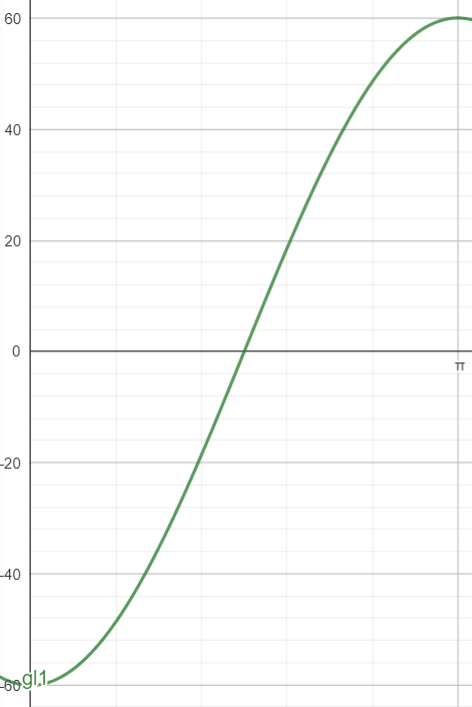
\includegraphics[width=5cm]{../ref/Rotationsmoment Elevation.png}
	\caption{Verlauf des Drehmoments über die Winkel 0-180°}
	\label{fig:verlauf-drehmoment}
\end{figure}

Es ist zu erwarten, dass das benötigte Rotationsmoment dann maximal ist, wenn der Rotor im 0° bzw. 180° Winkel steht. 
\begin{equation}
	M=23,32kg*9,81\frac{m}{s^2}*0,262705m*\sin(90°)=60,1Nm
\end{equation}

\begin{figure}[H]
	\begin{minipage}[b]{.4\linewidth} % [b] => Ausrichtung an \caption
		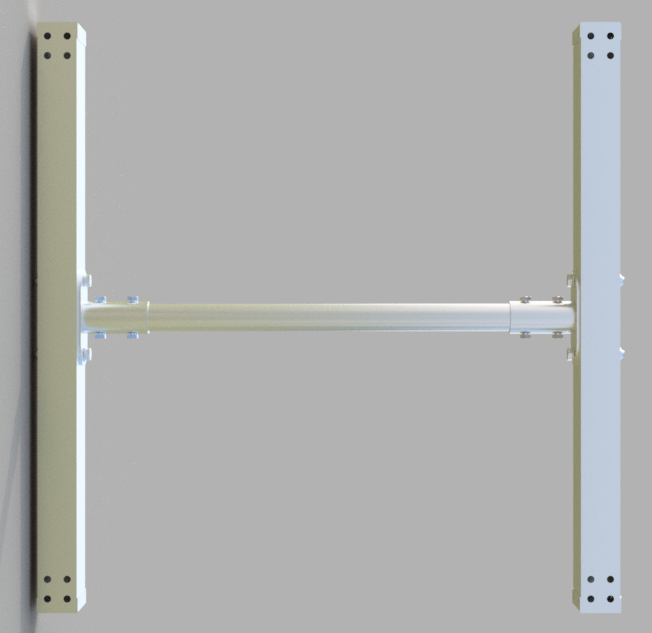
\includegraphics[width=\linewidth]{../ref/0000-Gesamtbaugruppe_Rahmen.png}
		\label{fig:Gerüst-Zeichnung}
	\end{minipage}
	\hspace{.1\linewidth}% Abstand zwischen Bilder
	\begin{minipage}[b]{.4\linewidth} % [b] => Ausrichtung an \caption
		\includegraphics[width=\linewidth]{../ref/Gerüst.jpg}
		\label{fig:Gerüst-real}
	\end{minipage}
	\caption{Gegenüberstellung des Renders zum realen Gerüst. In der realen Konstruktion sind bereits Teflonplatten montiert.}
\end{figure}

Um eine komplette elektrische Isolierung der Antennen vom Gerüst zu ermöglichen, kommen Teflonplatten zum Einsatz. Diese verbinden die Antennen mit dem Aluminium-Vierkantprofil.

\begin{figure}[H]
	\centering
	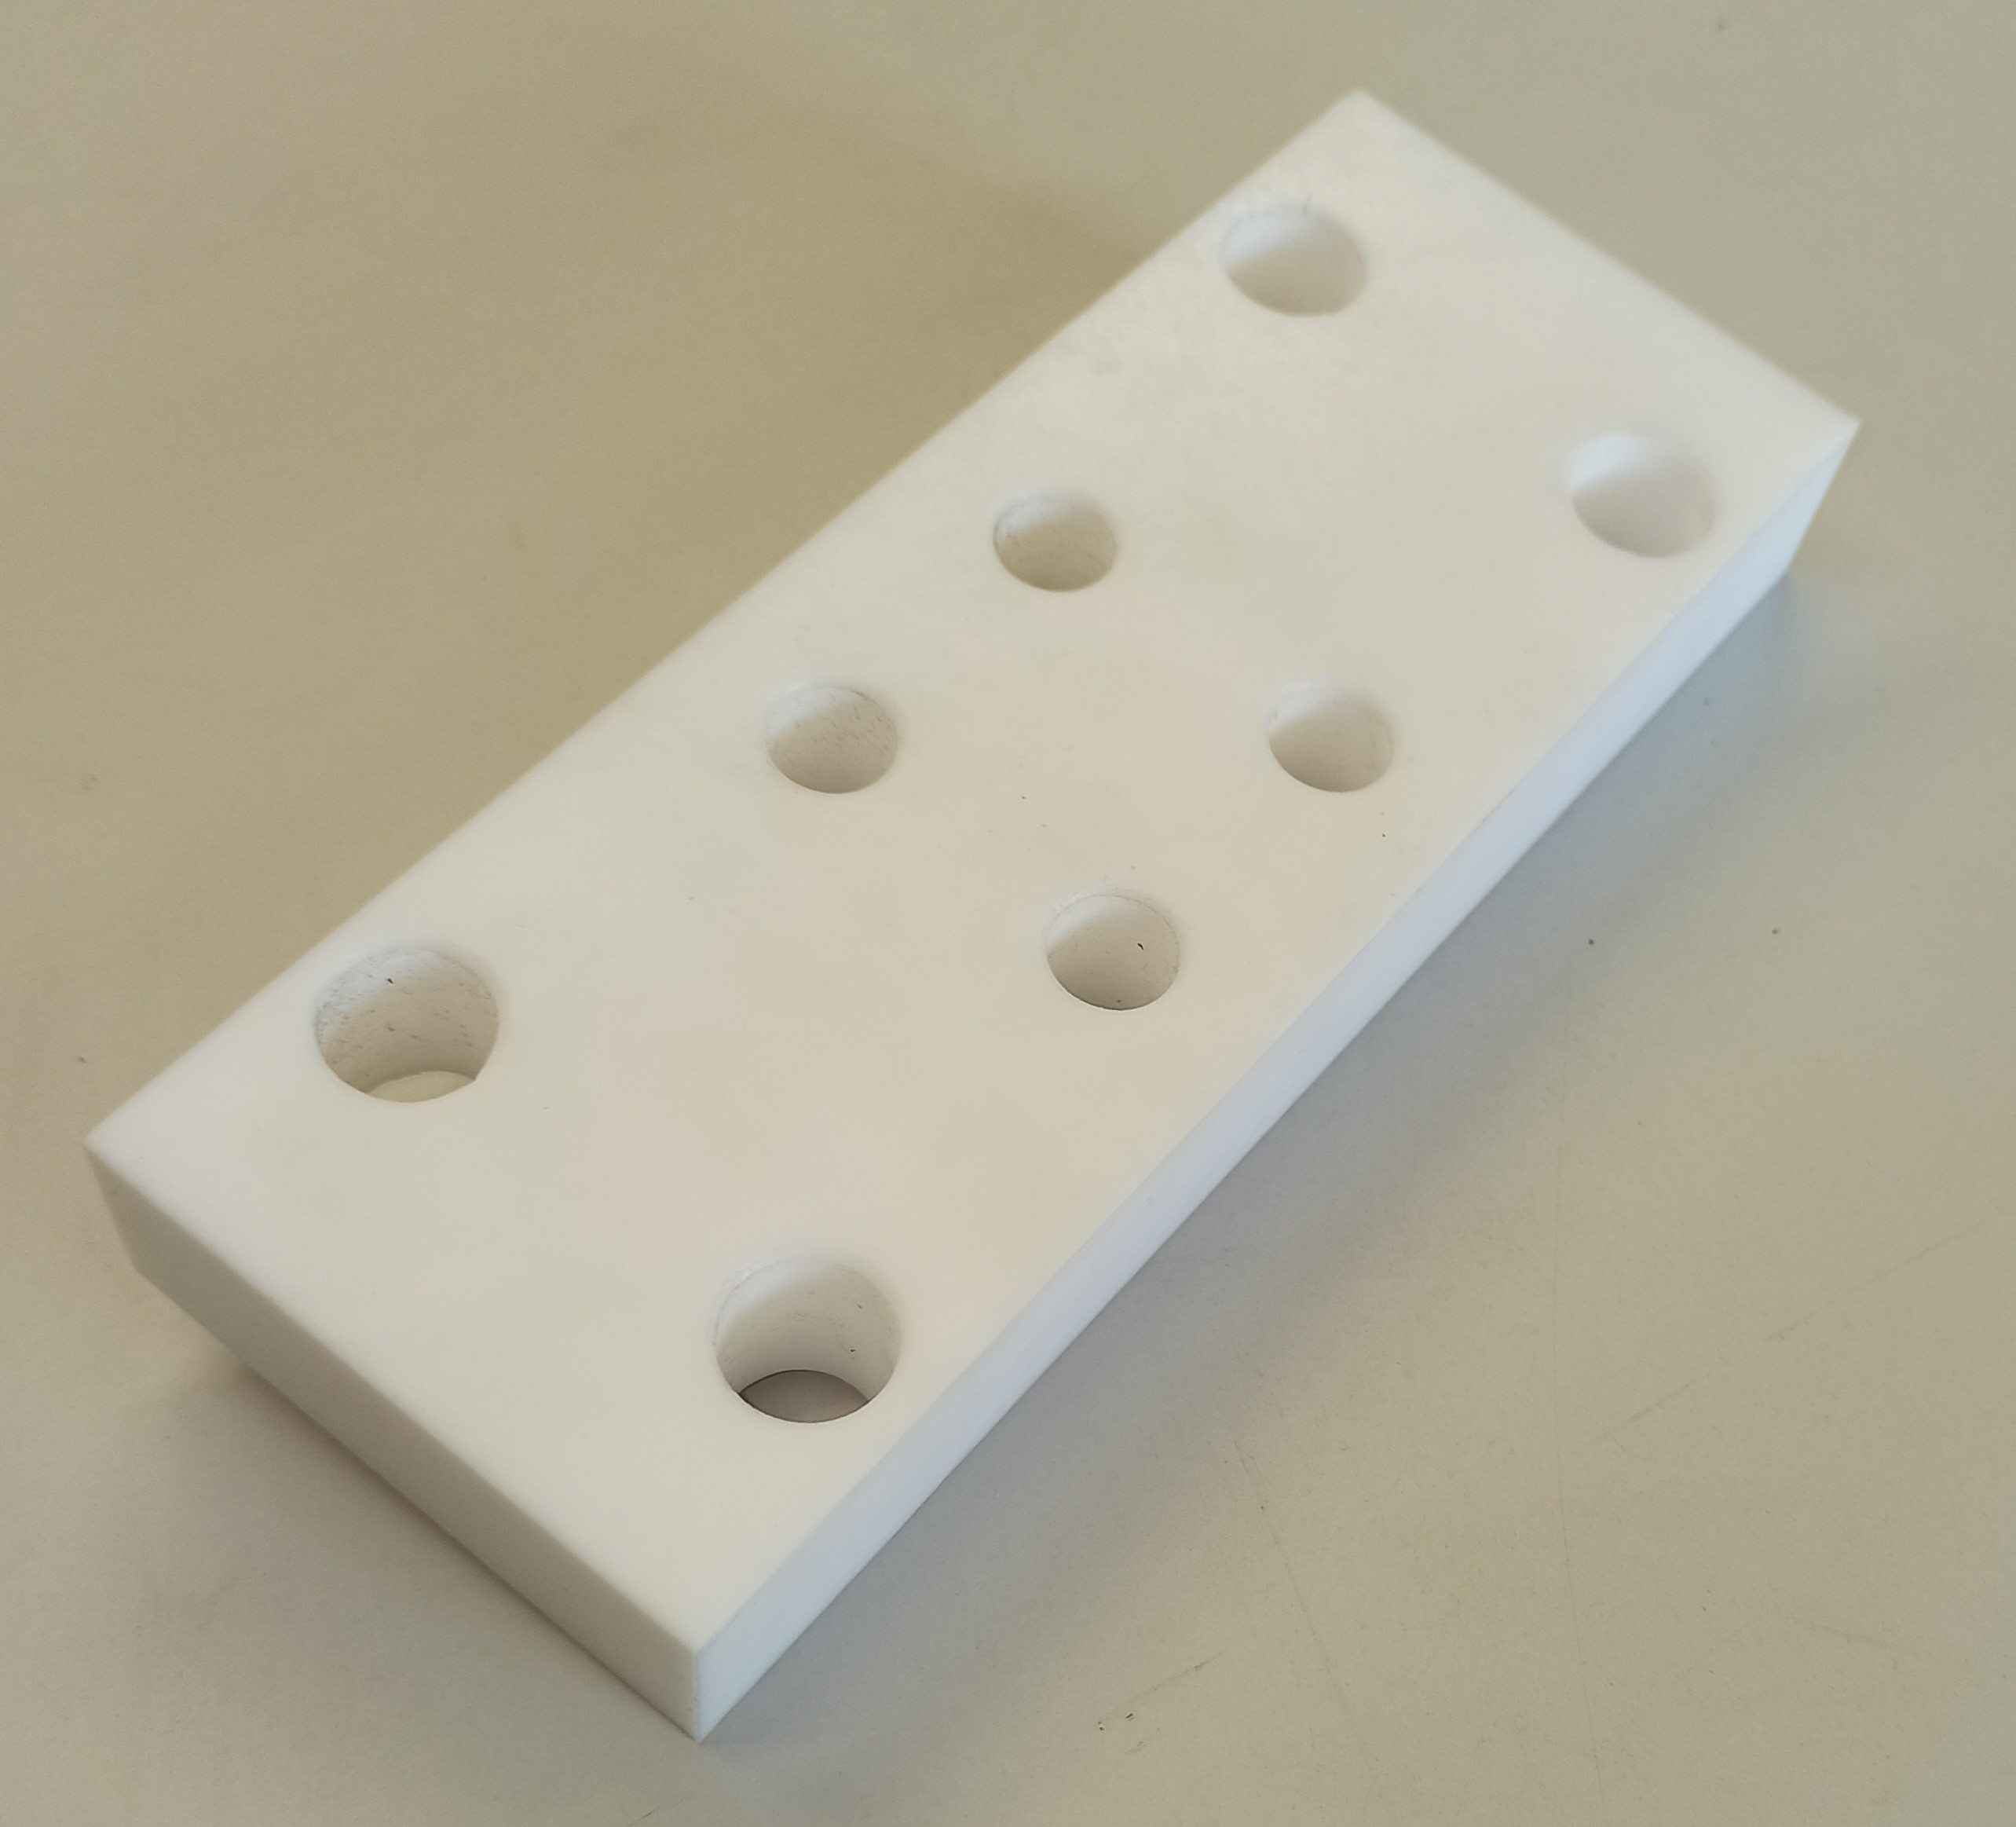
\includegraphics[width=5cm]{../ref/Teflon-Platte.jpg}
	\caption{Verbindende Teflonplatte}
	\label{fig:Teflonplatte}
\end{figure}

\subsection{Anpassung}
Da sich der Eingangswiderstand ändert, wenn vier solcher Antennen zusammen geschaltet werden, muss ein Anpassungsglied zwischen Koaxialkabel und Antennen eingesetzt werden. Hierfür wird ein $\lambda/4$-Anpasstopf gebaut. Dieser verhält sich ähnlich wie ein Koaxialkabel, wobei das Verhältnis der Durchmesser zwischen Innenleiter und Außenleiter die Kapazität festlegt. Hierdurch kann der Wellenwiderstand angepasst werden.

\begin{figure}[H]
	\centering
	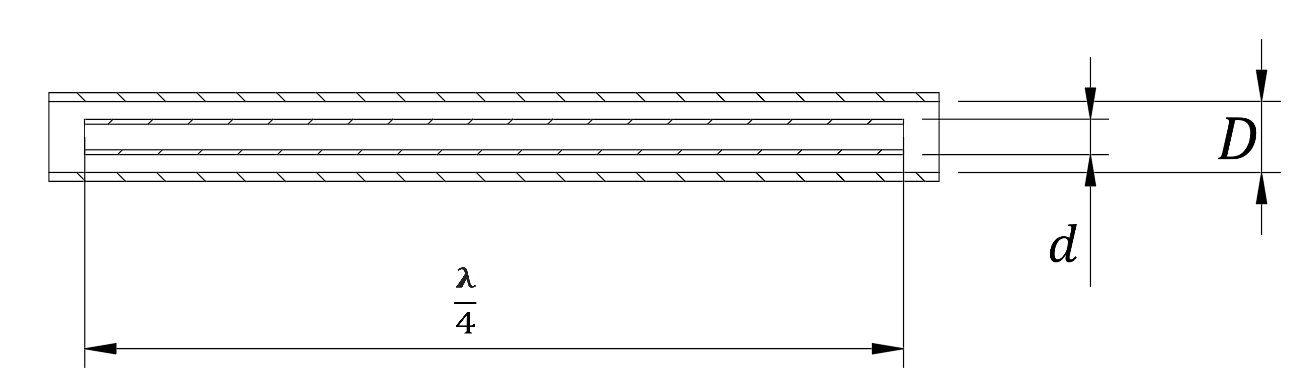
\includegraphics[width=\textwidth]{../ref/Prinzip-Anpasstopf.png}
	\label{fig:prinzip-anpasstopf}
	\caption{Querschnitt einer $\frac{\lambda}{4}$-Anpassleitung}
\end{figure}

Hierbei ist d der äußere Durchmesser des Innenleiters und D der innere Durchmesser des Außenleiters. Der Innenleiter ist $\frac{\lambda}{4}$ lang.

Für eine verlustlose $\frac{\lambda}{4}$-Leitung gilt:
\begin{equation}
	Z_E=\frac{(Z_W)^2}{Z_A}	
\end{equation}

Wobei $Z_E$ Der Eingangswiderstand des Anpasstopfes ist, $Z_A$ der Abschlusswiderstand und $Z_W$ der Wellenwiderstand der $\frac{\lambda}{4}$ Leitung \cite{admin_lambda4_2016}.

Um die Leitung korrekt zu dimensionieren muss zuerst der Wellenwiderstand ermittelt werden. Alle vier Helixantennen haben einen Antennenwiderstand von ca. 50$\Omega$. Werden diese parallel geschalten, so ergibt sich ein Gesamtwiderstand von 12,5$\Omega$. Da ein Koaxialkabel mit einem Wellenwiderstand von 50$\Omega$ verwendet wird, ist der Widerstand $Z_E$ 50$\Omega$. Somit ergibt sich durch umformen auf den Wellenwiderstand und einsetzen der Werte das nachfolgende Ergebnis \cite{admin_lambda4_2016}.

\begin{equation}
	Z_W=\sqrt{Z_E*Z_A}=\sqrt{12,5\Omega*50\Omega}=25\Omega
\end{equation}

Nun kann die Leitung dimensioniert werden. Es wurde ein viereckiger Außenleiter gewählt, da dies die Montage der BNC-Stecker vereinfacht. Um die Maße für die Leitung zu ermitteln, muss zuerst entweder der Durchmesser des Außenleiters oder des Innenleiters angenommen werden. Da ein 20x1.5mm Vierkantprofil verfügbar war, wurde dies als Außenleiter angenommen. Da der Innendurchmesser des Vierkantrohrs für die Kapazität relevant ist, wird $D=20mm-2*1,5mm=17mm$ gewählt. Daraus folgt für den Innenleiter:

\begin{equation}
	d=\frac{1,08*D}{10^{\frac{Z_W}{138}}}=\frac{1,08*17}{10^{\frac{25}{138}}}=12,09mm
\end{equation}


Es wird ein Kupferrohr mit einem Durchmesser von 12mm gewählt \cite{admin_lambda4_2016}.

Da die Maße feststehen, kann der Anpasstopf konstruiert werden. Es wurden als Addition Abdeckungen 3D-gedruckt.

\begin{figure}[H]
	\centering
	\begin{minipage}[b]{.2\linewidth} % [b] => Ausrichtung an \caption
		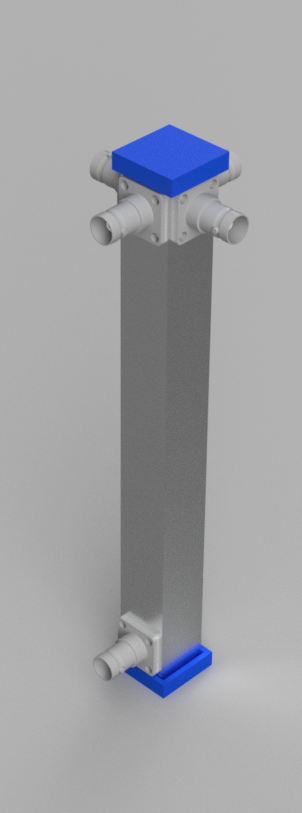
\includegraphics[width=\linewidth]{../ref/Lambda_4-Anpasstopf v1.png}
		\label{fig:Anpassleitung-Render}
	\end{minipage}
	\hspace{.1\linewidth}% Abstand zwischen Bilder
	\begin{minipage}[b]{.2\linewidth} % [b] => Ausrichtung an \caption
		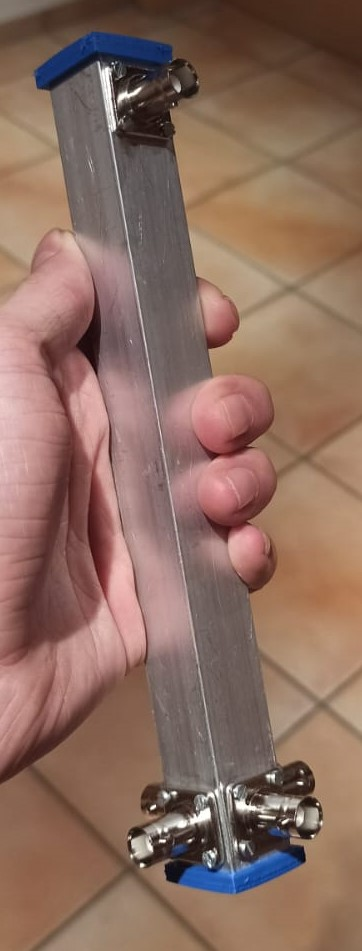
\includegraphics[width=\linewidth]{../ref/Anpasstopf-real.jpeg}
		\label{fig:Anpassleitung-real}
	\end{minipage}
	\caption{Gegenüberstellung des Renders zur realen Anpassleitung}
\end{figure}

\subsection{Messungen}
Um die Qualität des Antennenarrays zu überprüfen, wurde am Ausgang der $\frac{\lambda}{4}$-Anpassleitung gemessen. Hierbei werden der S11-Parameter, das SWR sowie das Smith-Diagramm analysiert, um qualitativ festzustellen, ob das Antennenarray funktionsfähig ist.

\begin{figure}[H]
	\centering
	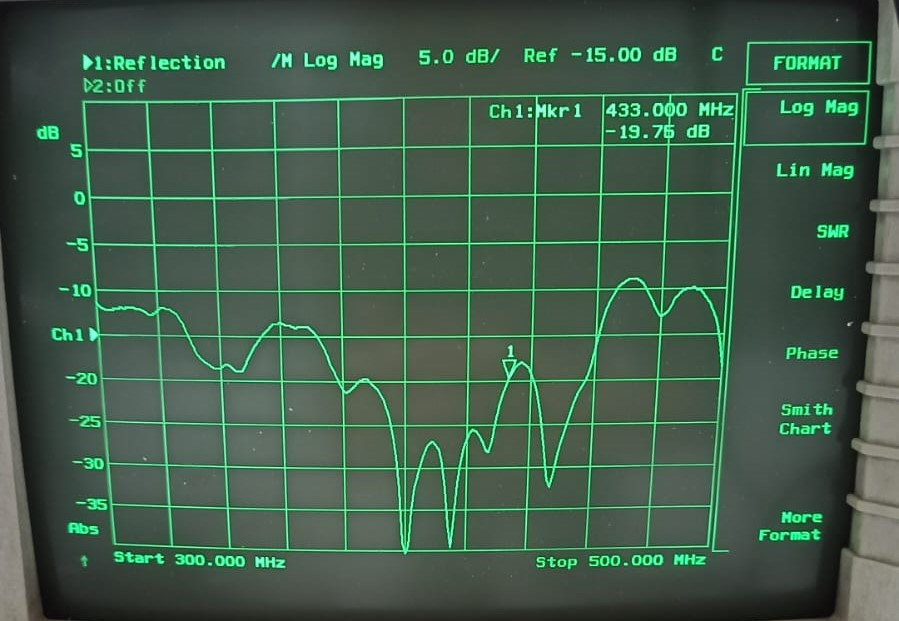
\includegraphics[width=10cm]{../ref/Array-S11.jpg}
	\label{fig:array-S11}
	\caption{S11-Parameter des Arrays}
\end{figure}

Anhand des S11-Parameters lässt sich feststellen, dass dieser mit einem Wert von ca. -20dB in einem relativ guten Bereich liegt.

\begin{figure}[H]
	\centering
	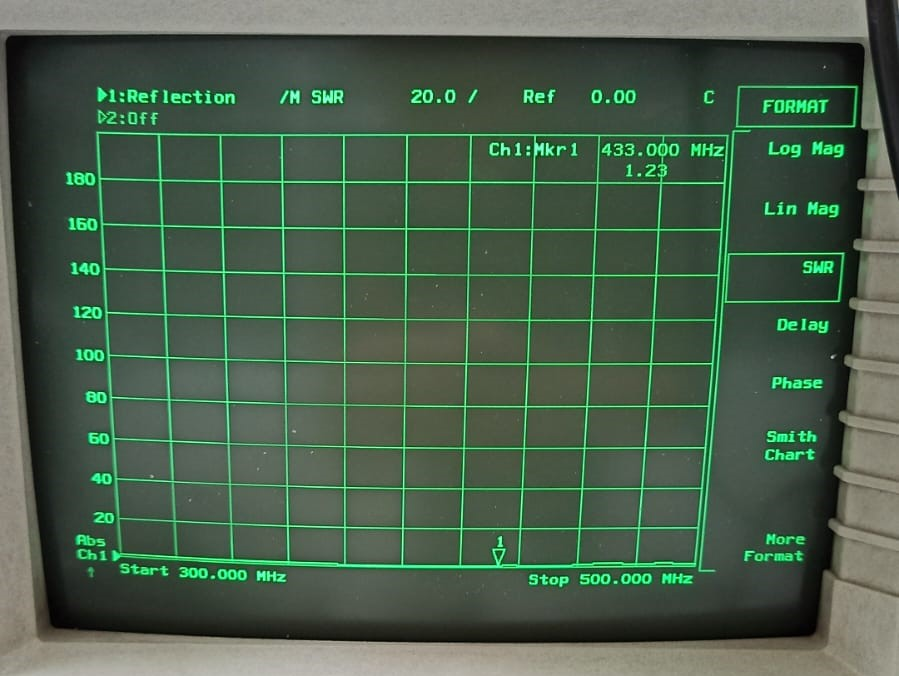
\includegraphics[width=10cm]{../ref/Array-SWR.jpg}
	\label{fig:array-SWR}
	\caption{SWR des Arrays}
\end{figure}

Mithilfe des SWRs kann ebenfalls auf die Güte der Anpassung geschlossen werden. Hier liegt der Wert ungefähr bei 1,2, was ein akzeptabler Wert ist.

\begin{figure}[H]
	\centering
	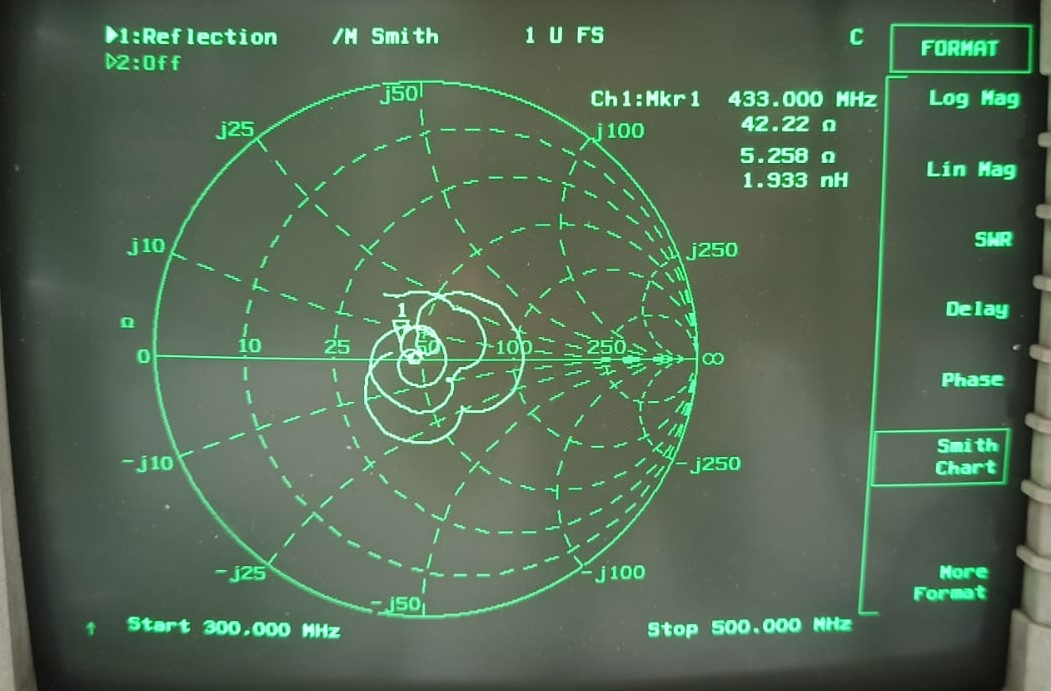
\includegraphics[width=10cm]{../ref/Array-Smith.jpg}
	\label{fig:array-Smith}
	\caption{Smith-Diagramm des Arrays}
\end{figure}

Am Smith-Diagramm ist zu erkennen, dass die Eingangsimpedanz der Antenne kaum imaginär ist und mit 42 Ohm relativ gut im Mittelpunkt des Smith-Diagramms liegt.

\section{Test}
Um die Funktionalität des Helix-Arrays und des Rotors nachzuweisen, wurden mehrere Observationen durchgeführt. Dabei wurden die Signale der einzelnen Helix-Antennen mithilfe des $\lambda/4$-Anpasstopfes zu einem Signal zusammengeführt.

Die Observationen wurden am 16. März 2024, an den Koordinaten 47.27139319984484, 9.63248486985336 (Negrellistraße 50, 6830 Rankweil), auf einer Höhe von 459 Metern über dem Meeresspiegel, durchgeführt.  Die Ergebnisse der Observationen, die zum Test der Funktionalität durchgeführt wurden, können unter folgendem Link aufgerufen werden:\newline \url{https://network.satnogs.org/observations/?norad=&start=2024-03-16+00%3A01&end=2024-03-17+20%3A59&observer=&station=3307&transmitter_mode=&transmitter_uuid=}

Mit 29 empfangenen Paketen empfing die Observation mit der Nummer 9209920 des Satelliten \glqq 53106 - GREENCUBE\grqq{}  und dem Sender \glqq Mode U TLM 1k2 GMSK\grqq{} die meisten Datenpakete. Die Daten wurden am 16. März 2024 von 13:39:27 bis 13:51:27 (UTC) empfangen. Die nachfolgende Abbildung zeigt das Wasserfalldiagramm sowie das erste dekodierte Datenpaket im HEX und ASCII Format.

\begin{figure} [H]
	\centering
	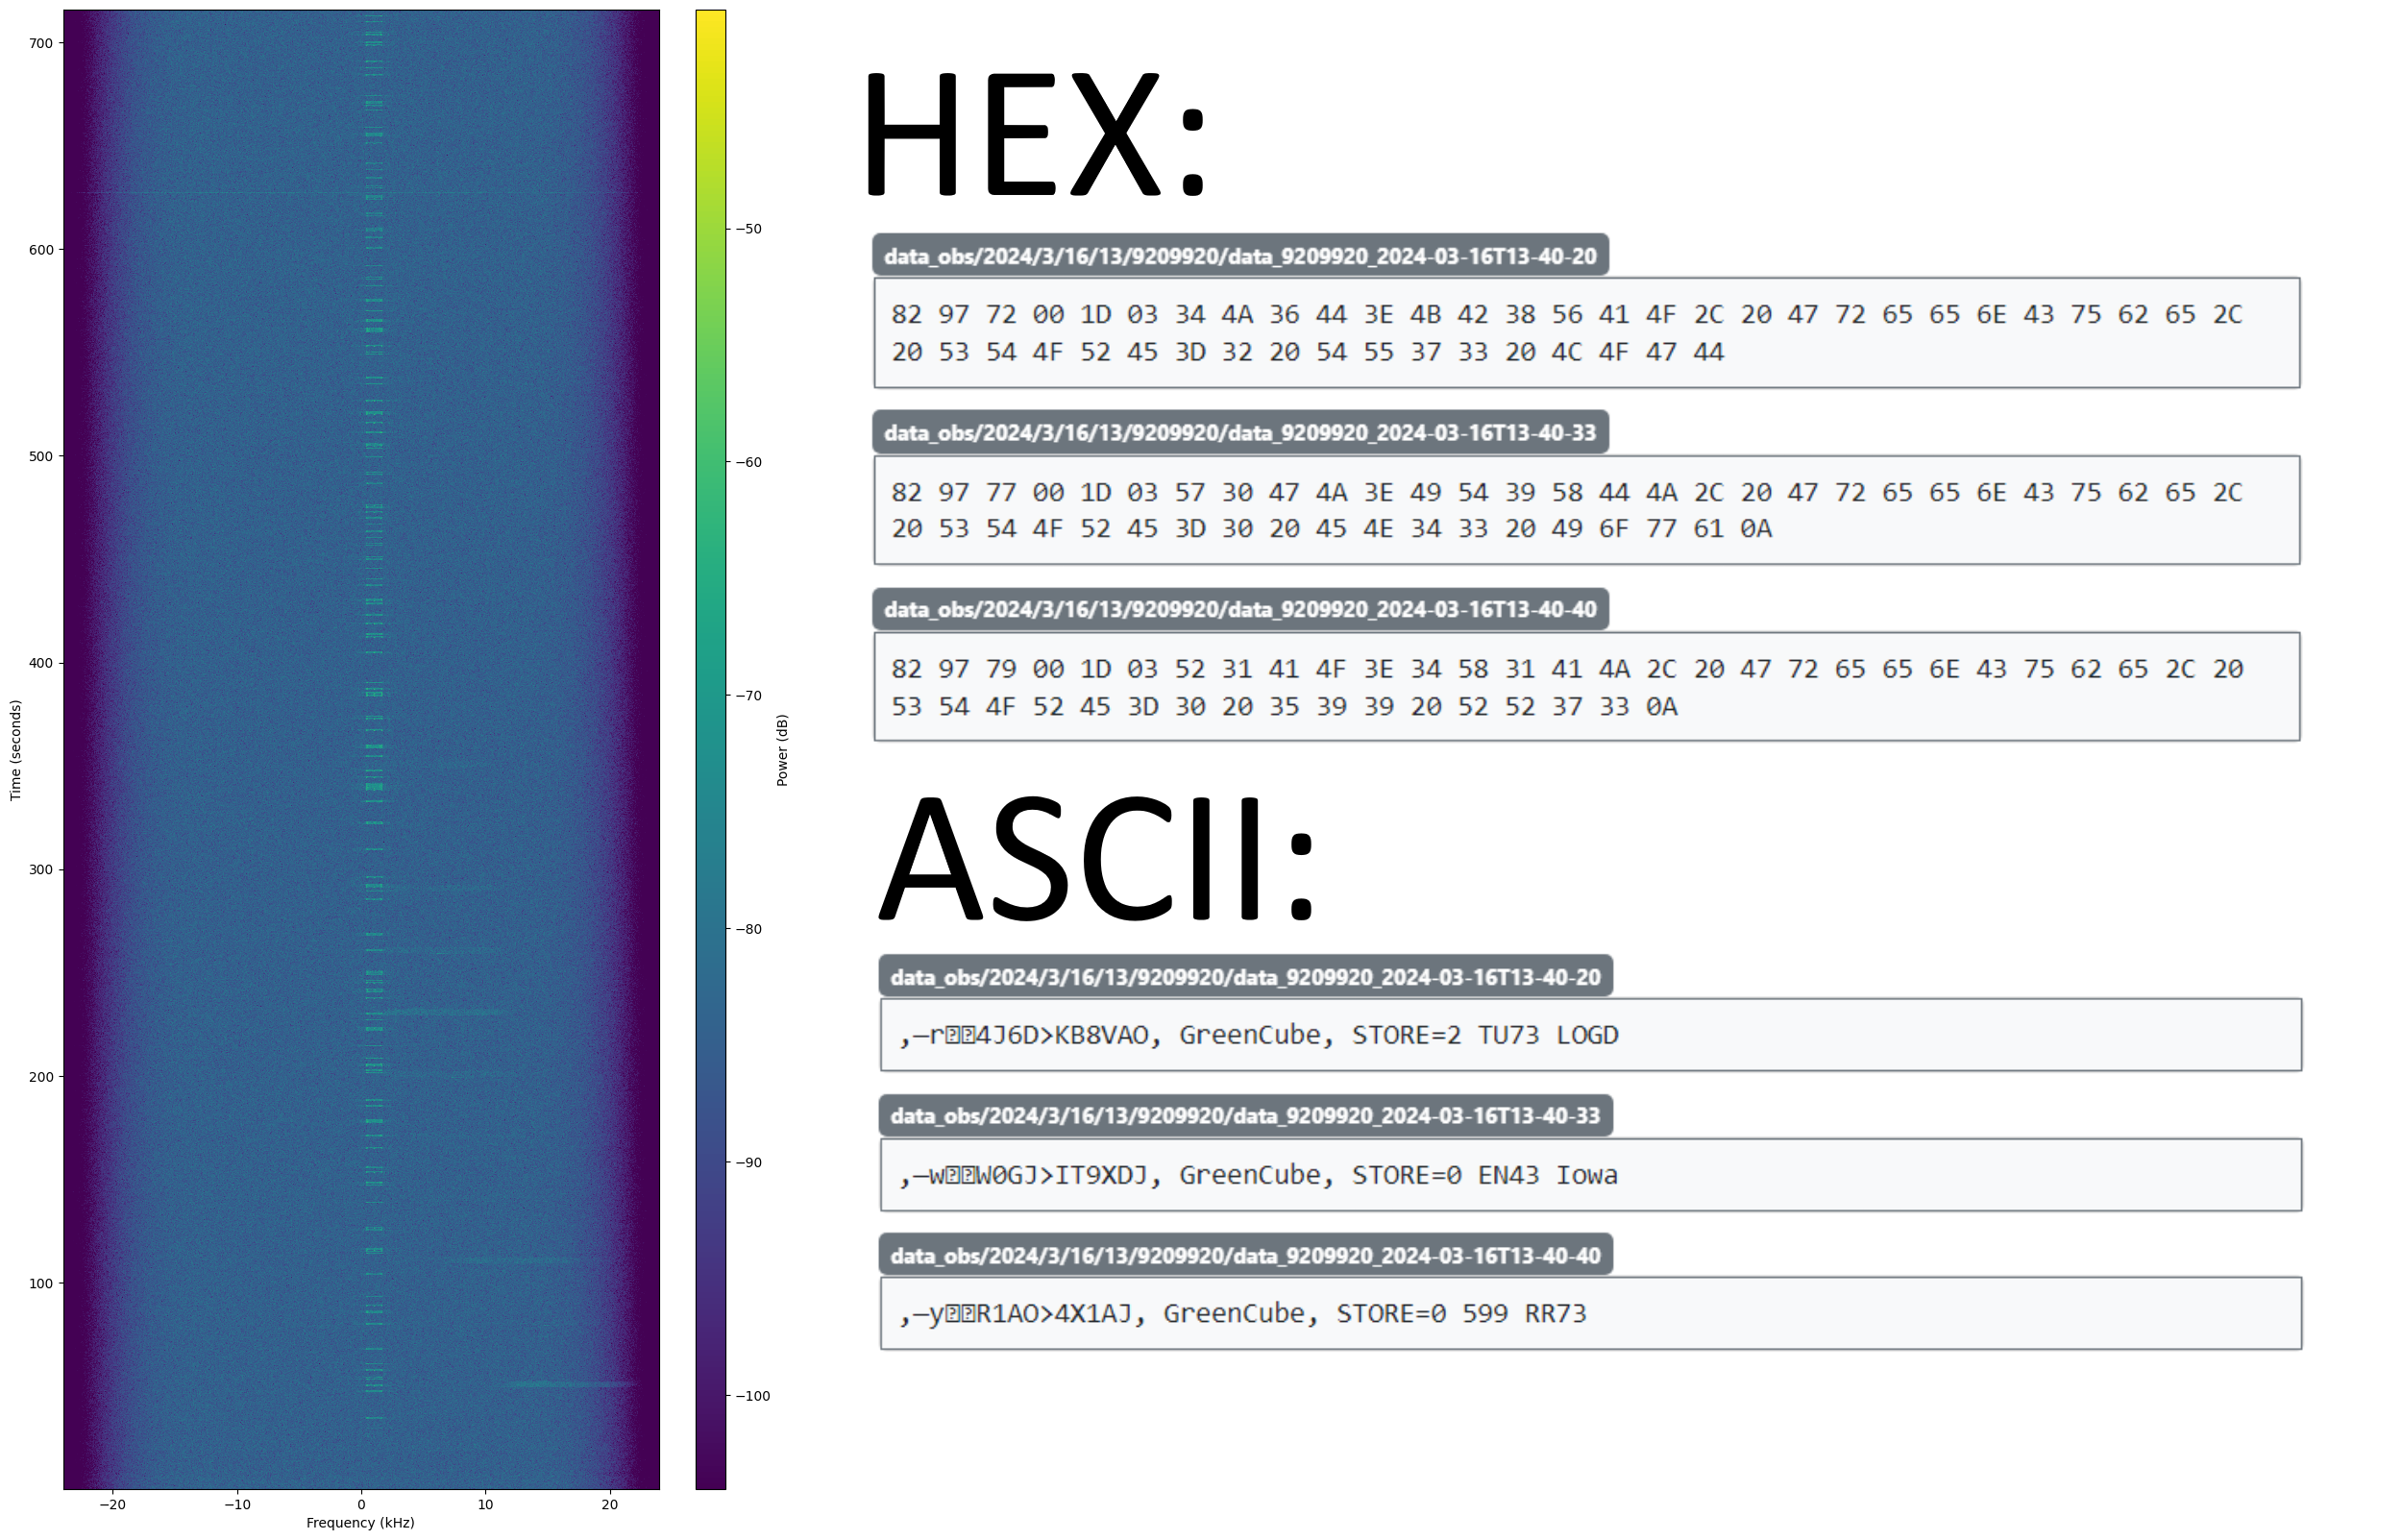
\includegraphics[width=\linewidth]{../ref/helix_successfull_observation.png}
	\caption{Wasserfalldiagramm und erstes Datenpaket in HEX und ASCII Format der Observation 9209920 \cite{noauthor_satnogs_observation_helix_nodate}}
	\label{fig:helix_successfull_observation}
\end{figure}
	\newpage
	\SecAuth{\emplLastA}
	\fancyfoot[LO,RE]{\DADate~\textbar~SatNOGS-Bodenstation~\textbar ~\@SecAuth}
	\chapter{Empfangsstation}
Als Empfangsstation wird das Gesamtsystem bezeichnet welches alle Komponenten beinhaltet die für den Empfang von Satellitendaten benötigt werden. In diesem Kapitel soll das Zusammenspiel der Komponenten und die Funktionsweise bisher noch unbehandelter Komponenten geklärt werden.

\section{Betriebsmittelkennzeichnung}
\label{sec:bmk}
Um alle Objekte innerhalb des Systems jederzeit eindeutig identifizieren zu können werden diese nach OVE EN IEC 81346-2 einer Referenzkennzeichnung unterzogen. Die benötigten Kennbuchstaben sind:

\begin{tabular}{|c|l|}
	\hline
	\textbf{Kennbuchstabe} & \textbf{Zweck oder Aufgabe nach EN IEC 81346-2} \\
	\hline
	A & zwei oder mehr Zwecke - kein identifizierbarer Hauptzweck \\
	\hline
	K & Verarbeiten von Signalen oder Informationen \\
	\hline
	M & Bereitstellen von mechanischer Energie zu Antriebszwecken \\
	\hline
	T & Umwandeln von Energie unter Beibehaltung der Energieart \\
	\hline
	W & Leiten oder Führen von Energie \\
	\hline
	X & Verbinden von Objekten \\
	\hline
\end{tabular}

Zur weiteren Differenzierung werden Ortskennzeichen angewandt. Die verwendeten Symbole und ihre Bedeutung lauten dadurch:

\begin{tabular}{|c|l|}
	\hline
	\textbf{Symbol} & \textbf{Bedeutung} \\
	\hline
	- & Betriebsmittel \\
	\hline
	+ & Ort \\
	\hline
\end{tabular}

Im Zuge dieses Kennzeichnungsprozesses ergibt sich folgende Zuordnung:

\begin{tabular}{|l|c||l|c|}
	\hline
	\textbf{Betriebsmittel} & \textbf{Kennzeichnung} & \textbf{Betriebsmittel} & \textbf{Kennzeichnung} \\
	\hline
	Schaltschrank & -A01 & Schuko 2 & +A01-X02 \\
	\hline
	Helix-Gerüst (\ref{subsec:helix_geruest}) & -A03 & Rotor (Azimut) (\ref{sec:yaesug5500dc}) & +A03-M01 \\
	\hline
	QFH-Antenne (\ref{chap:qfh}) & -T01 & Rotor (Elevation) (\ref{sec:yaesug5500dc}) & +A03-M02 \\
	\hline
	Raspberry Pi 4 QUERVERWEIS & +A01-A02 & RF-Power-Combiner (\ref{chap:helix}) & +A03-T04 \\
	\hline
	Rotor-Controller (\ref{sec:yaesug5500dc}) & +A01-K01 & Helix-Antenne 1 (\ref{chap:helix}) & +A03-T11 \\
	\hline
	GS232-Interface Emulation (\ref{sec:gs232emulation}) & +A01-K02 & Helix-Antenne 2 (\ref{chap:helix}) & +A03-T12 \\
	\hline
	SDR QUERVERWEIS & +A01-K03 & Helix-Antenne 3 (\ref{chap:helix}) & +A03-T13 \\
	\hline
	Netzteil & +A01-T03 & Helix-Antenne 4 (\ref{chap:helix}) & +A03-T14 \\
	\hline
	Netzkabel & +A01-W01 & Antennenkabel Helix 1 & +A03-W08 \\
	\hline
	USB-Kabel & +A01-W02 & Antennenkabel Helix 2 & +A03-W09 \\
	\hline
	5V-Kabel & +A01-W03 & Antennenkabel Helix 3 & +A03-W10 \\
	\hline
	DIN-Kabel & +A01-W04 & Antennenkabel Helix 4 & +A03-W11 \\
	\hline
	Azimut-Kabel & +A01-W05 & Antennenkabel Array & +A03-W12 \\
	\hline
	Elevation-Kabel & +A01-W06 & LNA  & +T01-T02 \\
	\hline
	Schuko1 & +A01-X01 & Antennen-Kabel & +T01-W07 \\
	\hline
\end{tabular}

Die in vorhergehenden Kapiteln noch nicht erwähnten Betriebsmittel und ihre Funktion werden nun im Zuge dieses Kapitels erläutert. 

\section{Schaltschrank (+A01)}
Die Aufgabe des Schaltschranks ist es, abgesehen von der Antennen, dem Rotor und des LNAs alle weiteren Komponenten der Empfangsstation vor UV-Strahlung und Wetter zu schützen. Ein weitere positiver Effekt der sich dadurch ergibt, ist die Flexibilität die ein solcher Schaltschrank bietet. Positionswechsel der Bodenstation erfordern somit nur den Transport der Antenne und des Schaltschranks und können mit geringerer Anzahl an ein- und ausstecken der Kabel durchgeführt werden.

Als Schaltschrank wird ein Stahlblech-Wandgehäuse der Argentina Reihe des Unternehmens IDE ELECTRIC, S.L. mit Außenmaßen von 400mm Höhe, 400mm Breite und 250mm Tiefe verwendet. Mit einer im Datenblatt \cite{ide_electric_sl_datenblatt_nodate} angegebenen IP66 Schutzklasse und UV-Schutz-Beschichtung erfüllt er die Voraussetzungen, um den von der Umwelt ausgehenden mechanischen Belastungen standzuhalten. Die erste Kennziffer der IP66 Schutzklasse garantiert Staubdichtigkeit und die zweite Kennziffer Schutz gegen starkes Strahlwasser und Überflutung \cite{lienig_elektronische_2014} (Seite 53).

\subsection{Befestigung der Komponenten}
Zur Befestigung der Komponenten dient eine mit dem Schaltschrank mitgelieferte 2 Millimeter Montageplatte aus verzinktem Stahlblech. Für die Montage der Schuko-Steckdosen, des Netzteils, der GS232-Emulation und des Raspberry Pi 4 wird auf dieses Stahlblech eine DIN-Schiene geschraubt, welche das einfache Aufstecken dieser Komponenten ermöglicht. Für den Arduino Uno der GS232-Emulation und den Raspberry Pi 4 wurden dafür passende Gehäuse erworben. Die Schuko-Steckdosen und das Netzteil sind bereits für diese Montageart kompatibel. 

Der Rotor-Controller ist die einzige Komponente im Schaltschrank welche nicht über eine DIN-Schiene befestigt wird. Für die Befestigung des Rotors wurde mithilfe eines 2 Millimeter dicken Eisenblechs ein Regal gebogen auf welchem der Rotor-Controller Platz findet. Um den Controller gegen verrutschen zu sichern wird er mithilfe eines gebogenen viereckigen Eisenringes festgespannt. Der Vorteil dieser Befestigung ist, dass das Gehäuse des Rotor-Controllers nicht modifiziert werden musste, der Rotor-Controller mit wenig Aufwand aus dem Schaltschrank entfernt werden kann und dennoch fixiert an seinem Platz ist. Um die Sicherheit der Anwender und Anwenderinnen des Schaltschrankes zu gewährleisten, ist dieser zusätzlich an zwei Erdungspunkten mit dem Schutzleiter des Netzkabels verbunden.

\begin{figure}[H]
	\centering
	\includegraphics[width=0.7\linewidth]{../ref/Schaltschrank_Befestigung.jpg}
	\caption{Befestigungskonzept im Schaltschrank}
	\label{fig:schaltschrankbefestigung}
\end{figure}

\subsection{Anschlüsse am Schaltschrank}
Der Schaltschrank verfügt an der Außenseite über keinerlei Anschlüsse. Die Kabel für die Stromversorgung, Antenne und Rotoren verlaufen über Kabelverschraubungen nach außen um dort direkt verwendet werden zu können. 

\begin{figure}[H]
	\centering
	\includegraphics[width=0.7\linewidth]{../ref/Schaltschrank_Anschluss.jpeg}
	\caption{Anschlüsse am Schaltschrank}
	\label{fig:schaltschrankanschluesse}
\end{figure}

Die unbeschriftete Schraubverbindung in der Abbildung dient als Reserve für mögliche Erweiterungen.

\subsection{Standfüße}
Um den Schaltschrank flexibel platzieren zu können wurden zwei Standfüße aus 10 Millimeter Chromstahlblech zusammengeschweißt und mit Gummifüßen versehen. 

\begin{figure}[H]
	\centering
	\includegraphics[width=9cm]{../ref/Schaltschrank_Fuss.jpeg}
	\caption{Standfuß für den Schaltschrank}
	\label{fig:schaltschrankfuss}
\end{figure}

Das Ergebnis ist ein modular platzierbarer und vielseitiger Schaltschrank:

\begin{figure}[H]
	\begin{minipage}[b]{.4\linewidth}
		\includegraphics[width=\linewidth]{../ref/Schaltschrank_stehend_vorne.jpeg}
		\label{fig:schaltschrankstehendvorne}
		\caption{Schaltschrank stehend (Ansicht vorne)}
	\end{minipage}
	\hspace{.1\linewidth}% Abstand zwischen Bilder
	\begin{minipage}[b]{.4\linewidth} % [b] => Ausrichtung an \caption
		\includegraphics[width=\linewidth]{../ref/Schaltschrank_stehend_hinten.jpeg}
		\label{fig:schaltschrankstehendhinten}
		\caption{Schaltschrank stehend (Ansicht hinten)}
	\end{minipage}
\end{figure}

\section{Netzteil (+A01-T03)}
Für die Stromversorgung des Raspberry Pi 4 sowie des im GS232A/B verbauten Arduino Uno wird das Schaltnetzteil S8VK-G01505 der OMRON Corporation verwendet. Das Netzteil kann mit einer Eingangsspannung von 100 bis 240 Volt und 50 Hertz betrieben werden und sorgt für eine Ausgangsspannung von 5 Volt. Mit einer maximalen Ausgangsleistung von  15 Watt ist es ausreichend groß dimensioniert um sowohl den Raspberry Pi 4 \cite{noauthor_power_nodate} als auch den Arduino Uno \cite{noauthor_r3_nodate} mit Strom zu versorgen. \cite{noauthor_s8vk-g01505_nodate}

\section{Netzkabel (+A01-W01)}
Das Netzkabel, mit einer Länge von 4.6 Metern außerhalb des Schaltschranks, versorgt die gesamte Empfangsstation mit Energie. Voraussetzung zum Betrieb der Empfangsstation ist es also, das Netzkabel mit einer Spannungsquelle (100 bis 120 oder 200 bis 240 Volt und 50 Hz) zu verbinden. Das verwendete Kabel ist ein H07BQ-F 3G1.5 der PATELEC Group \cite{noauthor_cables_nodate} und weißt dankt dem verwendeten Mantelmaterial Polyurethan eine gute UV-Beständigkeit auf \cite{noauthor_polyurethan_nodate}.

\section{USB-Kabel (+A01-W02)}
Das USB-Kabel ist ein USB-A zu USB-B Kabel und verbindet den Raspberry Pi 4 (USB-A) mit dem Arduino Uno (USB-B) der GS232-Interface Emulation. Abgesehen von der Kommunikation zwischen dem Raspberry Pi 4 und dem Arduino Uno, erfolgt auch die Stromversorgung des Arduinos über das USB-Kabel. Es handelt sich bei dem USB-Kabel um ein handelsübliches Kabel aus dem Eigenbestand ohne spezielle Eigenschaften, da es im Schaltschrank keinerlei mechanischen Belastung ausgesetzt ist.

\section{5V-Kabel (+A01-W03)}
Die Aufgabe des 5V-Kabels ist die Energieübertragung vom Netzteil zum Raspberry Pi 4. Die verwendete rot, schwarze Zwillingsleitung wird dazu vom Ausgang des Netzteils zu den auf dem Gehäuse des Netzteils angebrachten Verbindungsklemmen geführt. Der Zwischenschritt über die Verbindungsklemmen ermöglicht somit nicht nur eine leichteres Ein- und Ausbauen der Komponenten, sondern fördert auch die Skalierbarkeit im Bezug auf den Einbau weiterer elektronischer Komponenten welche eine 5 Volt Versorgungsspannung benötigen.

\begin{figure}[H]
	\centering
	\includegraphics[width=.25\linewidth]{../ref/Anschlussklemmen5V.jpeg}
	\caption{Anschlussklemmen 5 Volt Versorgung}
	\label{fig:anschlussklemmen}
\end{figure}

\section{DIN-Kabel (+A01-W04)}
Als DIN-Kabel wird in diesem Fall jenes Kabel bezeichnet, welches zur Verbindung der GS232-Interface Emulation zum G-5500DC Controller verwendet wird und an einem Ende einen 8-Pol DIN-Rundstecker aufweist. Die Zuordnung der Farben des Kabels zu den PIN-Nummern des Steckers, welche im Kapitel \ref{subsubsec:emulation_analoge_schnittstelle} genauer erläutert wurde, sowie die Zuordnung zu den Bezeichnungen auf dem Arduino-Shield, welche im Kapitel \ref{subsec:hardware} erklärt wurde, lautet wie folgt:

\begin{tabular}{c|c|c}
	\textbf{Farbe} & \textbf{Pin-Nummer} & \textbf{Bezeichnung am Arduino-Shield} \\
	\hline
	Grün & 1 & V \\
	Gelb & 2 & R \\
	Grau & 3 & U \\
	Weiß & 4 & L \\
	Blau & 5 & D \\
	Pink & 6 & H \\
	Rot & 7 & Vin \\
	Braun & 8 & GND \\
\end{tabular}

\section{Azimut-Kabel (+A01-W05)}
\label{sec:azimutkabel}
Das Azimut-Kabel dient zur Steuerung und Messung des Azimut-Rotors und wird im Kapitel \ref{subsubsec:kontrollkabel} als Kontrollkabel bezeichnet und seine Funktion genauer beschrieben. Mit einem Leiterquerschnitt von je 1.5 Millimetern erfüllt es die in Kapitel \ref{subsubsec:kontrollkabel} genannten Vorgaben und ist aufgrund des UV-Stabilisierten Außenmantels aus Polyvinylchlorid auch gegen irreparable Schäden durch Sonneneinstrahlung geschützt. Die Länge des Kabels außerhalb des Schaltschranks beträgt 4.8 Meter. 

\section{Elevation-Kabel (+A01-W06)}
Das Elevation-Kabel ist das Pendant zum Azimut-Kabel und dient der Steuerung und Messung des Elevation-Rotors. Die Eigenschaften entsprechen dem Kapitel \ref{sec:azimutkabel}.

\section{Schuko 1 (+A01-X01)}
\label{sec:schuko1}
Die Schutzkontaktsteckdose dient der Energieversorgung von Geräten mit Netzstecker. Das verwendete Modell SD35DEA des Unternehmen SHC GmbH verfügt über eine grüne Status-LED, die leuchtet, sobald das Netzkabel des Schaltschranks an eine Energiequelle angeschlossen wird. Die Schutzkontaktsteckdose Schuko 1 ist als Reserve für mögliche weitere Geräte oder für temporäre Anwendungen wie z.B. das Laden eines Notebooks oder dem Ausleuchten des Schaltschranks eingebaut.

\section{Schuko 2 (+A01-X02)}
Die Schutzkontaktsteckdose Schuko 2 weist dieselben technischen Eigenschaften wie die Schutzkontaktsteckdose 1, welche in Kapitel \ref{sec:schuko1} beschrieben wird, auf. Die Schutzkontaktsteckdose Schuko 2 ist für die Energieversorgung des Yeasu G-5500DC Controllers vorgesehen, kann allerdings auch für jegliche andere Geräte verwendet werden.

\section{Antennenkabel Helix und Array (+A03-W09 bis W12)}
Die Antennenkabel +A03-W09 bis W12 des Typ RG58 C/U führen von den Antennen zum RF-Combiner mit einer Länge von insgesamt 1.25m pro Kabel. Entsprechend der RG58 C/U Bezeichnung weisen die Kabel einen Wellenwiderstand von 50 Ohm sowie \cite{noauthor_rg_nodate} eine Dämpfung von 0.3 Dezibel pro Meter bei 400 Megahertz \cite{noauthor_vergleich_nodate}. 

\section{LNA (+T01-T02)}
Die Leistung einer Antenne lässt sich in einer Gütezahl angeben die als gain-to-noise-temperature, kurz G/T, bezeichnet wird. Diese G/T ist eine positive Zahl die mit steigender Performanz der Antenne zunimmt. Um diese zu verbessern muss entweder der Gewinn der Antenne vergrößert oder der relative Rauschanteil im Signal verringert werden. Weil das Vergrößern des Gewinns einer omnidirektionalen Antenne sich als sehr schwierig gestaltet und in den meisten Fällen in einer gerichteten Antenne mündet, muss der Rauschanteil abnehmen. Um dies zu tun wird das Wideband LNA von RTL-SDR.com in der Signalkette direkt nach der Antenne verwendet. Im Vergleich zum SDR, welches ursprünglich alleine die Aufgabe hatte das Signal der Antenne zu Verstärken, weist das Wideband LNA mit 0.52 Dezibel bei 800 MHz eine sehr geringe Rauschzahl auf. \cite{noauthor_new_nodate} \cite{noauthor_omnidirectional_nodate}

\begin{figure}[H]
	\centering
	\includegraphics[width=.75\linewidth]{../ref/wideband_lna_gain.png}
	\caption{Verstärkung des Wideband LNAs in Abhängigkeit der Frequenz \cite{noauthor_new_nodate}}
	\label{fig:wideband_lna_gain}
\end{figure}

Die Verstärkung des Wideband LNAs entspricht laut gezeigter Grafik des Herstellers etwa 22.5 Dezibel bei 433 Megahertz.

\section{Antennen-Kabel (+T01-W07)}
Das Antennen-Kabel +T01-W07 wird für die Verbindung des SDR mit dem Ausgang des LNAs verwendet und weist eine Länge von insgesamt 3 Metern auf. Das Kabel entspricht dem Typ RG174 und weist somit neben einer Wellenimpedanz von 50 Ohm eine Streckendämpfung von 0.7 Dezibel pro Meter bei 432 Megahertz auf \cite{noauthor_dunnes_nodate}.

\section{Prinzipschaltplan}
Der nachfolgende Prinzipschaltplan dient dem Zweck, Anwenderinnen und Anwendern einen guten Überblick über die verbaute Hardware und dessen Verkabelung zu bekommen. Hierzu wurden die, im Rahmen der Betriebsmittelkennzeichnung in Kapitel \ref{sec:bmk}, festgelegten Kennzeichnungen im Prinzipschaltplan berücksichtigt, sowie die Komponenten in Realität dementsprechend beschriftet.

\begin{landscape}
	\begin{figure}
		\centering
		\includegraphics[width=\linewidth]{../ref/Prinzipschaltplan.jpg}
		\caption{Prinzipschaltplan der Empfangsstation}
		\label{fig:prinzipschaltplan}
	\end{figure}
\end{landscape}

\section{Observation planen}
\subsection{Voraussetzung}
Um eine Observation mit der Empfangsstation planen zu können, wird Benutzerkonto im SatNOGS Netzwerk mit der entsprechenden Berechtigung benötigt. Folgende Matrix erläutert die möglichen Aktionen die gemäß der Art des Benutzerkontos durchgeführt werden können.

\begin{figure} [H]
	\centering
	\includegraphics[width=\linewidth]{../ref/network_permission_matrix.png}
	\caption{SatNOGS Netzwerkberechtigungsmatrix \cite{noauthor_operation_nodate}}
	\label{fig:networkpermissionmatrix}
\end{figure}

\subsection{Observation auswählen}
Auf der Seite der Empfangsstation (hier: https://network.satnogs.org/stations/3307/) können über den Reiter \textbf{Future Passes}  die in der Zukunft passierenden Satelliten angezeigt werden.

\begin{figure} [H]
	\centering
	\includegraphics[width=\linewidth]{../ref/schedule_observation_futurepass.png}
	\caption{Landingpage HTLR-UHF(Test) Empfangsstation \cite{noauthor_satnogs_nodate}}
	\label{fig:htrl-uhf(test)landingpage}
\end{figure}

Die folgende Abbildung zeigt die zukünftig passierenden Satelliten und ausgewählte Informationen über die potenzielle Observation.

\begin{figure} [H]
	\centering
	\includegraphics[width=\linewidth]{../ref/schedule_observation_infos.png}
	\caption{HTLR-UHF(Test) Empfangsstation - zukünftige Passierungen \cite{noauthor_satnogs_nodate}}
	\label{fig:htrl-uhf(test)futurepasses}
\end{figure}

Entsprechend der Beschriftung geben die Informationen Aufschluss über folgende Eigenschaften:

\textbf{1}: Status der bereits betätigten Observation. Wobei Grün für Erfolgreich, Orange für unbewertet, Rot für Fehlgeschlagen und Blau für zukünftig steht.\newline

\textbf{2}: Beginn des Signalempfangs (AOS - Acquisition of Signal) \newline

\textbf{3}: Zeitpunkt des Signalverlusts (LOS - Loss of Signal) \newline

\textbf{4}: von oben nach unten: Azimut zum Zeitpunkt AOS, Azimut zum Zeitpunk der geringsten Entfernung vom Satellit zur Empfangsstation, Azimut zum Zeitpunkt LOS \newline

\textbf{5}: Der Polar-Plot zeigt den Elevationswinkel (Entfernung zum Mittelpunkt) sowie den Azimutalwinkel (Angegeben durch die Himmelsrichtungen) während der Observation an. Der grüne Punkt Kennzeichnet den AOS-Zeitpunkt und der rote Punkt den LOS-Zeitpunkt.

Über den mit \textbf{6} markierten Button kann die Observation in einem weiteren Fenster, wie in nachfolgender Grafik gezeigt, konfiguriert und durchgeführt werden.

\begin{figure} [H]
	\centering
	\includegraphics[width=\linewidth]{../ref/schedule_observation_schedule.png}
	\caption{HTLR-UHF(Test) Empfangsstation - Observation konfigurieren und starten} \cite{noauthor_satnogs_nodate}
	\label{fig:htrl-uhf(test)configureobservation}
\end{figure}

Das mit \textbf{1} markierte Dropdown-Menü zeigt den zur Observation ausgewählten Satelliten an und über das mit \textbf{2} markierte können die vorhandenen Sender des Satelliten angezeigt und ausgewählt werden. Mithilfe der mit \textbf{4} markierten Eingabefelder kann Start- und Endzeitpunkt der Observation konfiguriert werden. Das mit \textbf{3} markierte Feld zeigt die zur Observation ausgewählte Empfangsstation an. Mit einem Klick auf den mit \textbf{5} markierten Button \textbf{Schedule} wird die Observation geplant und startet automatisch zum konfigurierten Zeitpunkt.

\subsection{Observation auswerten}
Um die Observationen einer Empfangsstation anzuzeigen wird auf den in der nächsten Grafik mit \textbf{1} markierten Button auf der Landingpage der Empfangsstation gedrückt.

\begin{figure} [H]
	\centering
	\includegraphics[width=\linewidth]{../ref/show_observation.png}
	\caption{HTLR-UHF(Test) Empfangsstation - Observationen anzeigen} \cite{noauthor_satnogs_nodate}
	\label{fig:htrl-uhf(test)showobservations}
\end{figure}

Die somit erschienene Übersicht zeigt alle mit dieser Station getätigten und zukünftigen Observationen an.

\begin{figure} [H]
	\centering
	\includegraphics[width=.75\linewidth]{../ref/overview_observations.png}
	\caption{HTLR-UHF(Test) Empfangsstation - Übersicht Observationen} \cite{noauthor_satnogs_nodate}
	\label{fig:htrl-uhf(test)overviewobservations}
\end{figure}

Durch das Klicken auf eine Observation öffnet sich eine weitere Seite die sowohl die allgemeinen Informationen zur Observation als auch die Ergebnis in Form eines Wasserfalldiagramms, einer Audiospur sowie dekodierter Daten enthält. 

\begin{figure} [H]
	\centering
	\includegraphics[width=\linewidth]{../ref/vet_observation.png}
	\caption{HTLR-UHF(Test) Empfangsstation - Observation auswerten} \cite{noauthor_satnogs_nodate}
	\label{fig:htrl-uhf(test)vetobservation}
\end{figure}

Ist im Wasserfalldiagramm ein dem Transmitter-Mode entsprechendes Signal zu erkennen, so kann die Observation dementsprechend über die mit \textbf{1} markierten Buttons bewertet werden.



	\newpage
	\SecAuth{\emplLastA}
	\fancyfoot[LO,RE]{\DADate~\textbar~SatNOGS-Bodenstation~\textbar ~\@SecAuth}
	\chapter{Projektmanagement}
In diesem Kapitel werden alle in der Grundstruktur der Diplomarbeit nicht behandelten Aspekte der Projektplanung erläutert. Dazu gehören die Finanzplanung und dementsprechende Sponsorensuche und die Kommunikation im Team. 
\section{Finanzplanung}
Ausreichend liquide Mittel sind Voraussetzung für die erfolgreiche Durchführung der Diplomarbeit. Um diese Voraussetzung zu erfüllen wurde mithilfe einer Broschüre der Diplomarbeit nach Sponsoren gesucht. Im Rahmen dieser Sponsorensuche haben sich 3 Sponsoren gefunden die das Projekt mit insgesamt € 862.54 finanziell unterstützen. Weitere großzügige Sponsoren unterstützten das Projekt mit Materialien und Dienstleistungen und senkten so die Gesamtkosten. Folgende Ausgaben wurden im Rahmen der Diplomarbeit getätigt:

\begin{tabular}{|c|c|c|}
	\hline
	\textbf{Beschreibung} & \textbf{Kosten} & \textbf{Übernommen von} \\
	\hline
	RTL-SDR Blog V3 USB Dongle with Dipole Antenna Kit &  € 69,54  & Jakob Metzler \\
	\hline
	Raspberry Pi 4 8GB &  € 93,00  & Jakob Metzler \\
	\hline
	Yeasu G5500 Antenna Rotator &  € 750,00  & Gabriel Ritter \\
	\hline
	Gehäuse für Arduino &  € 13,33  & Jakob Metzler \\
	\hline
	Gehäuse für Raspberry Pi 4 &  € 14,11  & Jakob Metzler \\
	\hline
	Arduino für Steuereinheit Rotator &  € 9,88  & Jakob Metzler \\
	\hline
	PCB für Steuereinheit Rotator &  € 3,92  & Jakob Metzler \\
	\hline
	Crimpzange + Stecker &  € 26,21  & Jakob Metzler \\
	\hline
	RF Power Splitter 50 Ohm &  € 5,23  & Jakob Metzler \\
	\hline
	SMA-Connector Male-Male 5 Stück &  € 14,11  & Jakob Metzler \\
	\hline
	Rohrhalter UV-beständig 50 Stk. &  € 50,59  & Gabriel Ritter \\
	\hline
	PVC Rohr UV-beständig 4m &  € 27,38  & Gabriel Ritter \\
	\hline
	Kunststoffschrauben M6x15mm 50 Stück &  € 9,65  & Jakob Metzler \\
	\hline
	Kunststoffmuttern M10 100 Stück &  € 14,82  & Jakob Metzler \\
	\hline
	Kunststoffschrauben M6x20mm 50 Stück &  € 10,38  & Jakob Metzler \\
	\hline
	Kunststoffschrauben M6x20mm 50 Stück &  € 7,88  & Jakob Metzler \\
	\hline
	Wilkinson-Combiner Bauteile &  € 27,52  & Jakob Metzler \\
	\hline
	SMA-Leitplattenbuchse &  € 6,00  & Jakob Metzler \\
	\hhline{|===|}
	\textbf{Insgesamt} & \multicolumn{2}{c|}{€ 1.164,01} \\
	\hline
\end{tabular}

Die Kosten die somit nicht durch die Sponsorings gedeckt wurden betragen \textbf{€ 301,47} und wurden vom Projektteam übernommen. 

\section{Kommunikation}
Die Kommunikation in einem Team nimmt starken Einfluss auf dessen Effizienz. Um diese Effizienz zu bewahren, wurden innerhalb des Teams regelmäßige Gespräche geführt, um auf dem neuesten Stand zu bleiben und sich über Probleme auszutauschen. Diese Gespräche haben sich als sehr nützlich erwiesen und fanden in den meisten Fällen während der 45-minütigen Hin- und Rückfahrt zur Schule statt. 
	\newpage
	\SecAuth{\emplLastA}
	\fancyfoot[LO,RE]{\DADate~\textbar~SatNOGS-Bodenstation~\textbar ~\@SecAuth}
	\chapter{Conclusio}

Mit dem Abschluss der Diplomarbeit wurden die gesteckten Ziele erfolgreich erreicht und wichtige Erkenntnisse gewonnen. Die Arbeit präsentiert ein funktionierendes Konzept für den Bau einer Empfangsstation im globalen Satellitenkommunikationsnetzwerk SatNOGS, das die flächenmäßige Abdeckung erweitert und die Ausfallsicherheit erhöht.

Die Erfahrungen aus dem Bau der quadrifilaren Helixantenne erwiesen sich als äußerst wertvoll beim Bau der monofilaren Helixantenne, was zu einem ausgereiften Antennenarray führte. Unter Berücksichtigung des finanziellen Aspekts ist festzustellen, dass selbst bei geringerem finanziellen Aufwand, wie es bei einer quadrifilaren Helixantenne der Fall ist, eine zuverlässige Antenne und somit eine erschwingliche Empfangsstation für den Empfang von Daten wissenschaftlicher Satelliten realisiert werden kann.

In Anbetracht der Kosteneffizienz der quadrifilaren Helixantenne ist es sinnvoll, ihre Entwicklung fortzusetzen. Dies könnte durch eine eingehende Untersuchung und Analyse der Abweichungen zwischen der gemessenen Richtwirkung und den Simulationsergebnissen erfolgen, sowie durch die Prüfung der Auswirkungen der Form des Materials zur Modellierung der Schleifen auf die Antenneneigenschaften.

Die im Pflichtenheft festgelegte Dekodierung und Darstellung der empfangenen Daten für den CubeSat des TU Wien Space Team konnte nicht durchgeführt werden, da das dafür benötigte Protokoll noch nicht vollständig vom Space Team entwickelt wurde.
	\newpage
	
	% -------------------------- 
	% Back matter
	% --------------------------
	\SecAuth{\emplLastA, \emplLastB}
	\fancyfoot[LO,RE]{\DADate~\textbar~SatNOGS-Bodenstation~\textbar ~\@SecAuth}
	
	\pdfbookmark[0]{Vorwort}{Vorwort}
\chapter*{Vorwort}
\label{chap:Vorwort}
%\vspace*{5cm}
Unsere Diplomarbeit nahm ihren Lauf als einige freundliche Mitglieder des TU-Wien-Space-Teams auf unsere Schule zu kamen und uns ein Projekt vorstellten: eine Bodenstation zum Empfang von Daten eines Satelliten der 2024 in den LEO befördert werden sollte - des STS1.\\
\newline
Dies weckte unser Interesse, bald fanden wir uns in einem Team wieder das hochmotiviert und bereit war loszulegen. 

	\newpage
	\addcontentsline{toc}{chapter}{10 Abbildungsverzeichnis}
	\listoffigures
	\setcounter{chapter}{10}
	\newpage
	\chapter{Literaturverzeichnis}
\vspace{1cm}
\printbibliography[heading=none]
	\newpage
	\SecAuth{\emplLastA}
	\fancyfoot[LO,RE]{\DADate~\textbar~SatNOGS-Bodenstation~\textbar ~\@SecAuth}
	\chapter{Fortschrittsbericht}

\section{Ritter Gabriel}

\begin{longtable}{|l|c|c|}
	\hline
	\textbf{Tätigkeit} & \textbf{Datum} & \textbf{Dauer} \\
	\hline
	Besprechen Diplomarbeitsantrag & 18.09.2023 & 03:40:00 \\
	\hline
	Dokumentation Grundstruktur erstellt & 25.09.2023 & 02:00:00 \\
	\hline
	Recherche QFH & 02.10.2023 & 03:40:00 \\
	\hline
	Firmenpartner anschreiben & 04.10.2023 & 01:40:00 \\
	\hline
	SatNOGS Netzwerk beschreiben & 09.10.2023 & 03:40:00 \\
	\hline
	SatNOGS Netzwerk beschreiben & 10.10.2023 & 01:00:00 \\
	\hline
	Recherche Baluns & 06.10.2023 & 01:00:00 \\
	\hline
	Antennen Funktionsweise beschreiben & 16.10.2023 & 03:40:00 \\
	\hline
	Fortführung Dokumentation & 18.12.2023 & 02:40:00 \\
	\hline
	Antennen Funktionsweise beschreiben & 23.10.2023 & 03:40:00 \\
	\hline
	Berechnung QFH & 01.11.2023 & 03:40:00 \\
	\hline
	Sponsorengespräch \& Messkammer organisieren (Omicron) & 08.11.2023 & 02:00:00 \\
	\hline
	Firmenpartner anschreiben & 23.11.2023 & 01:00:00 \\
	\hline
	Wellentheorie beschreiben & 04.12.2023 & 01:57:00 \\
	\hline
	Recherche CCSDS-Protokoll & 08.12.2023 & 01:00:00 \\
	\hline
	Recherche CCSDS-Protokoll & 09.12.2023 & 01:00:00 \\
	\hline
	Modellierung Schutzabdeckung Rotorsteuerung & 18.12.2023 & 01:00:00 \\
	\hline
	Dokumentation Vorlage erstellt & 29.12.2023 & 01:00:00 \\
	\hline
	Dokumentation Vorlage erstellt & 31.12.2023 & 01:45:00 \\
	\hline
	Dokumentation Vorlage erstellt & 01.01.2024 & 01:45:00 \\
	\hline
	Dokumentation Vorlage erstellt & 02.01.2024 & 00:55:00 \\
	\hline
	Vorwort erstellt \& Design sowie Struktur überarbeitet & 03.01.2024 & 01:00:00 \\
	\hline
	3D-Modell der Helix Antenne designt & 06.01.2024 & 04:00:00 \\
	\hline
	3d-Modell der Helix Antenne überarbeitet & 08.01.2024 & 01:30:00 \\
	\hline
	Helix-Antenne Theorie besprochen & 08.01.2024 & 03:40:00 \\
	\hline
	Schrack Vertrag ausgedruckt \& weitere Sponsoren geklärt & 12.01.2024 & 01:00:00 \\
	\hline
	Helix-Antenne überarbeitet (Aluminium + keine Kollisionen) & 13.01.2024 & 01:00:00 \\
	\hline
	Vorlage-Emails verfasst & 13.01.2024 & 01:55:00 \\
	\hline
	Präsentation SatNOGS + Helix-Antenne bearbeitet & 15.01.2024 & 04:05:00 \\
	\hline
	Präsi + Modifikationen an Helix-Antenne & 16.01.2024 & 01:00:00 \\
	\hline
	Präsentation weiter bearbeitet & 20.01.2024 & 01:00:00 \\
	\hline
	Präsentation fertiggestellt + Stichwortzettel & 21.01.2024 & 01:00:00 \\
	\hline
	Weitere Sponsoren angefragt & 23.01.2024 & 00:30:00 \\
	\hline
	Konstruktion für Helix-Antennen-Array & 23.01.2024 & 03:30:00 \\
	\hline
	Yaesu-G5500DC STL Modell zusammengefügt & 24.01.2024 & 00:30:00 \\
	\hline
	Helix-Strukturbolzen weitergearbeitet & 24.01.2024 & 01:00:00 \\
	\hline
	Helix finalisiert & 24.01.2024 & 03:30:00 \\
	\hline
	Helix Montageplatte modelliert & 25.01.2024 & 01:30:00 \\
	\hline
	QFH getestet & 25.01.2024 & 03:00:00 \\
	\hline
	Bauteile für Helix-Antenne herausgesucht & 26.01.2024 & 01:00:00 \\
	\hline
	Bauteile für Helix-Antenne herausgesucht & 26.01.2024 & 01:00:00 \\
	\hline
	Bauteile für Helix-Antenne herausgesucht & 27.01.2024 & 01:00:00 \\
	\hline
	Bauteile für Helix-Antenne herausgesucht & 27.01.2024 & 00:30:00 \\
	\hline
	Helix-Antenne weiter bearbeitet + Bauteile herausgesucht & 28.01.2024 & 02:30:00 \\
	\hline
	Weitere Sponsoren angefragt & 29.01.2024 & 01:00:00 \\
	\hline
	Helix-Antennen-Array bearbeitet & 29.01.2024 & 01:00:00 \\
	\hline
	Helix Antenne ideal rekonstruiert & 29.01.2024 & 04:12:00 \\
	\hline
	Helix-Antenne neu konstruiert & 30.01.2024 & 01:00:00 \\
	\hline
	Helix-Antenne neu konstruiert & 30.01.2024 & 01:00:00 \\
	\hline
	Helix-Antenne neu konstruiert + Leistungsanpassung informiert & 31.01.2024 & 00:45:00 \\
	\hline
	Helix-Antenne neu konstruiert & 04.02.2024 & 00:10:00 \\
	\hline
	Dokumentation weitergeführt & 10.02.2024 & 01:30:00 \\
	\hline
	Informationsbeschaffung + Materialbeschaffung & 11.02.2024 & 01:15:00 \\
	\hline
	Dokumentation weitergeführt & 11.02.2024 & 00:30:00 \\
	\hline
	Dokumentation weitergeführt & 11.02.2024 & 01:00:00 \\
	\hline
	Informationsbeschaffung zu Antennentheorie & 12.02.2024 & 00:30:00 \\
	\hline
	Informationsbeschaffung zu Antennentheorie & 15.02.2024 & 01:00:00 \\
	\hline
	Informationsbeschaffung zu Helix-Antennen & 18.02.2024 & 01:00:00 \\
	\hline
	Sponsoren vorbereitet & 19.02.2024 & 01:15:00 \\
	\hline
	QFH getestet & 19.02.2024 & 02:45:00 \\
	\hline
	Kunststoff bei SenTech für Helix-Antenne abholen & 19.02.2024 & 01:20:00 \\
	\hline
	Referenzen in Latex repariert & 19.02.2024 & 01:00:00 \\
	\hline
	Dokumentation zur Helix fertiggestellt & 20.02.2024 & 00:30:00 \\
	\hline
	Dokumentation zur Helix fertiggestellt & 20.02.2024 & 01:27:00 \\
	\hline
	Seitenelement erstellt & 21.02.2024 & 00:30:00 \\
	\hline
	Seitenelement erstellt & 21.02.2024 & 00:45:00 \\
	\hline
	Dokumentation zur Helix weitergeführt & 21.02.2024 & 00:55:00 \\
	\hline
	Dokumentation zur Helix weitergeführt & 22.02.2024 & 00:20:00 \\
	\hline
	Theorie Helix weitergeführt & 22.02.2024 & 01:00:00 \\
	\hline
	Theorie Helix weitergeführt & 22.02.2024 & 02:00:00 \\
	\hline
	Recherche Impedanzanpassung Helix & 22.02.2024 & 01:00:00 \\
	\hline
	Dokumentation weitergeführt & 23.02.2024 & 00:30:00 \\
	\hline
	Dokumentation weitergeführt & 24.02.2024 & 01:05:00 \\
	\hline
	Dokumentation weitergeführt & 24.02.2024 & 01:06:00 \\
	\hline
	Dokumentation weitergeführt & 24.02.2024 & 01:06:00 \\
	\hline
	Dokumentation weitergeführt & 25.02.2024 & 01:05:00 \\
	\hline
	Dokumentation weitergeführt & 25.02.2024 & 01:17:00 \\
	\hline
	Dokumentation weitergeführt & 25.02.2024 & 01:15:00 \\
	\hline
	Seitenelemente zugeschnitten + gedreht & 26.02.2024 & 04:00:00 \\
	\hline
	Dokumentation weitergeführt & 27.02.2024 & 01:00:00 \\
	\hline
	Dokumentation weitergeführt & 27.02.2024 & 00:30:00 \\
	\hline
	Informationssammlung Selbstphasenmodulation & 29.02.2024 & 00:30:00 \\
	\hline
	Dokumentation Theorie QFH & 01.03.2024 & 01:00:00 \\
	\hline
	Dokumentation Theorie QFH & 01.03.2024 & 00:26:00 \\
	\hline
	Informationssammlung Montage Helicalantenne & 02.03.2024 & 01:00:00 \\
	\hline
	Helixantennen-Array Montage & 02.03.2024 & 08:00:00 \\
	\hline
	Dokumentation & 03.03.2024 & 00:30:00 \\
	\hline
	Helixantennen-Array Messung und Tests & 04.03.2024 & 04:40:00 \\
	\hline
	Dokumentation & 04.03.2024 & 02:20:00 \\
	\hline
	Dokumentation & 05.03.2024 & 00:30:00 \\
	\hline
	Dokumentation & 05.03.2024 & 01:00:00 \\
	\hline
	Dokumentation & 05.03.2024 & 01:30:00 \\
	\hline
	Dokumentation + PVC Abdeckung designt & 05.03.2024 & 03:00:00 \\
	\hline
	Deckel neu designt + Dokumentation & 06.03.2024 & 00:30:00 \\
	\hline
	Helixantennen gemessen + Anpassstreifen neu dimensioniert & 06.03.2024 & 02:00:00 \\
	\hline
	Dokumentation & 06.03.2024 & 01:54:00 \\
	\hline
	Dokumentation & 07.03.2024 & 00:30:00 \\
	\hline
	Dokumentation & 07.03.2024 & 04:05:00 \\
	\hline
	Dokumentation & 08.03.2024 & 01:00:00 \\
	\hline
\end{longtable}

\section{Metzler Jakob}

\begin{longtable}{|l|c|c|}
	\hline
	\textbf{Tätigkeit} & \textbf{Datum} & \textbf{Dauer} \\
	\hline
	Besprechen Diplomarbeitsantrag & 18.09.2023 & 03:40:00 \\
	\hline
	Github Repository erstellen \& einrichten & 25.09.2023 & 00:14:00 \\
	\hline
	Kontaktieren möglicher Partner & 02.10.2023 & 00:30:00 \\
	\hline
	Monday.com einrichten & 03.10.2023 & 00:45:00 \\
	\hline
	Recherche Antennentypen & 04.10.2023 & 00:16:00 \\
	\hline
	Arbeitspakete erstellen & 04.10.2023 & 00:24:00 \\
	\hline
	Pflichtenheft erstellen & 02.10.2023 & 02:55:00 \\
	\hline
	Arbeitspakete erstellen & 06.10.2023 & 01:00:00 \\
	\hline
	Meilensteine definieren & 06.10.2023 & 00:30:00 \\
	\hline
	Arbeitspakete erstellen & 06.10.2023 & 00:28:00 \\
	\hline
	Arbeitspakete zuweisen & 06.10.2023 & 00:11:00 \\
	\hline
	Risikoplanung erstellen & 06.10.2023 & 00:25:00 \\
	\hline
	Pflichtenheft erstellen & 07.10.2023 & 00:20:00 \\
	\hline
	Pflichtenheft erstellen & 07.10.2023 & 00:55:00 \\
	\hline
	Recherche Antennentypen & 09.10.2023 & 00:46:00 \\
	\hline
	Recherche Baluns & 09.10.2023 & 02:54:00 \\
	\hline
	Recherche Baluns & 16.10.2023 & 01:30:00 \\
	\hline
	Pflichtenheft erstellen & 16.10.2023 & 01:31:00 \\
	\hline
	Recherche Antennentypen & 16.10.2023 & 00:29:00 \\
	\hline
	Recherche Baluns & 23.10.2023 & 03:25:00 \\
	\hline
	Registrierung im SatNOGS Netzwerk & 28.10.2023 & 03:41:00 \\
	\hline
	Sponsorengespräch \& Messkammer organisieren (Omicron) & 08.11.2023 & 02:00:00 \\
	\hline
	Fertigung der Antenne & 13.11.2023 & 03:40:00 \\
	\hline
	CAD-Plan für Antenne erstellen & 23.11.2023 & 01:45:00 \\
	\hline
	CAD-Plan für Antenne erstellen & 27.11.2023 & 03:40:00 \\
	\hline
	Sponsorengespräch \& Messkammer organisieren (Bachmann) & 28.11.2023 & 01:00:00 \\
	\hline
	Materialbeschaffung für Antenne & 30.11.2023 & 00:29:00 \\
	\hline
	Konzept Empfangsmodulhardware & 01.12.2023 & 01:51:00 \\
	\hline
	Materialbeschaffung für Empfangsmodulhardware & 04.12.2023 & 00:45:00 \\
	\hline
	CAD-Plan für Antenne erstellen & 04.12.2023 & 03:40:00 \\
	\hline
	Simulation \& Entwicklung QFH & 10.12.2023 & 07:08:00 \\
	\hline
	Simulation \& Entwicklung QFH & 17.12.2023 & 04:00:00 \\
	\hline
	Simulation \& Entwicklung QFH & 18.12.2023 & 02:35:00 \\
	\hline
	Materialbeschaffung für Antenne & 18.12.2023 & 01:05:00 \\
	\hline
	Assemblierung der Empfangsmodul-Hardware & 18.12.2023 & 02:20:00 \\
	\hline
	Fehlersuche Rotator & 26.12.2023 & 06:27:59 \\
	\hline
	Fehlersuche Rotator & 27.12.2023 & 01:30:00 \\
	\hline
	Fehlerbehebung Rotator \& Konfiguration & 27.12.2023 & 08:25:00 \\
	\hline
	Konfiguration Rotator & 28.12.2023 & 00:08:00 \\
	\hline
	Simulation \& Entwicklung QFH & 28.12.2023 & 02:45:00 \\
	\hline
	Assemblierung und Testen der Empfangsmodul-Hardware & 29.12.2023 & 01:33:00 \\
	\hline
	Bau der Antenne (QFH) & 07.01.2024 & 01:15:00 \\
	\hline
	Bau der Antenne (QFH) & 07.01.2024 & 04:17:00 \\
	\hline
	Bau der Antenne (QFH) & 08.01.2024 & 04:00:00 \\
	\hline
	Simulation der Helicoidal Antenne & 08.01.2024 & 01:31:00 \\
	\hline
	Bau der Antenne (QFH) & 09.01.2024 & 03:35:00 \\
	\hline
	Informations- und Teilbeschaffung für Antenna Array & 13.01.2024 & 02:44:00 \\
	\hline
	Konstruktion der Antenne + Planung Helicoidal Antenne & 15.01.2024 & 03:40:00 \\
	\hline
	Assemblierung der Hardware & 20.01.2024 & 05:15:00 \\
	\hline
	Zwischenpräsentation der Diplomarbeit & 22.01.2024 & 02:50:00 \\
	\hline
	Ausmessen der QFH & 25.01.2024 & 01:55:00 \\
	\hline
	Simulieren der Helix-Antenne & 28.01.2024 & 02:30:00 \\
	\hline
	Simlieren der Helix-Antenne & 28.01.2024 & 01:50:00 \\
	\hline
	QFH anpassen & 29.01.2024 & 04:15:00 \\
	\hline
	QFH anpassen & 05.02.2024 & 04:15:00 \\
	\hline
	Helix-Antenne simulieren & 08.02.2024 & 00:30:00 \\
	\hline
	QFH Reflexionsmessungen + Anpassen & 08.02.2024 & 05:25:00 \\
	\hline
	QFH Abdeckkappe zeichnen & 12.02.2024 & 01:00:00 \\
	\hline
	QFH Signal-Analyzer Messungen & 19.02.2024 & 02:20:00 \\
	\hline
	Kunststoff bei SenTech für Helix-Antenne abholen & 19.02.2024 & 01:20:00 \\
	\hline
	Kunstoff für Helix-Antenne bearbeiten & 27.02.2024 & 03:40:00 \\
	\hline
	Kunstoff für Helix-Antenne bearbeiten & 27.02.2024 & 01:40:00 \\
	\hline
	Dokumentation Rotor & 27.02.2024 & 01:59:59 \\
	\hline
	Dokumentation Rotor & 28.02.2024 & 00:01:00 \\
	\hline
	Dokumentation Rotor  & 28.02.2024 & 02:05:00 \\
	\hline
	Dokumentation Rotor & 29.02.2024 & 02:00:00 \\
	\hline
	Rohrklemmen bearbeiten & 29.02.2024 & 03:30:00 \\
	\hline
	Helix-Antennen Array Montage & 02.03.2024 & 09:00:00 \\
	\hline
	LNA-Gehäuse fertigen & 03.03.2024 & 00:45:00 \\
	\hline
	Helix-Antennen Array  in Transportfahrzeug laden & 03.03.2024 & 00:15:00 \\
	\hline
	Dokumentation Rotor & 03.03.2024 & 02:30:00 \\
	\hline
	Anpassung Helix-Antennen, Assemblierung Antennenmast & 04.03.2024 & 03:40:00 \\
	\hline
	Dokumentation Rotor & 04.03.2024 & 01:29:59 \\
	\hline
	Dokumentation Rotor & 05.03.2024 & 01:14:00 \\
	\hline
	Schaltung für diskreten RF-Combiner entwickeln  & 06.03.2024 & 01:35:00 \\
	\hline
	PCB für diskreten RF-Combiner erstellen \& Bauteile bestellen & 06.03.2024 & 01:14:59 \\
	\hline
	PCB für diskreten RF-Combiner erstellen \& Bauteile bestellen & 07.03.2024 & 02:20:00 \\
	\hline
	RF-Combiner bestücken & 07.03.2024 & 01:00:00 \\
	\hline
	Kabel konfektionieren, RF-Combiner testen & 11.03.2024 & 03:40:00 \\
	\hline
	Observationen mit QFH durchführen & 11.03.2024 & 03:45:00 \\
	\hline
	Dokumentation schreiben und Observationen durchführen & 12.03.2024 & 01:15:00 \\
	\hline
	Dokumentation schreiben & 12.03.2024 & 05:36:00 \\
	\hline
	Dokumentation schreiben & 12.03.2024 & 02:28:00 \\
	\hline
	Observationen planen (QFH) & 12.03.2024 & 00:20:00 \\
	\hline
	Dokumentation schreiben & 13.03.2024 & 07:23:00 \\
	\hline
	Feldmessung QFH & 14.03.2024 & 01:00:00 \\
	\hline
	Feldmessung QFH & 14.03.2024 & 03:45:00 \\
	\hline
	Dokumentation schreiben & 14.03.2024 & 05:29:59 \\
	\hline
	Dokumentation schreiben & 15.03.2024 & 03:21:00 \\
	\hline
	Dokumentation schreiben & 15.03.2024 & 04:10:00 \\
	\hline
	Dokumentation schreiben & 15.03.2024 & 04:59:59 \\
	\hline
	Dokumentation schreiben & 16.03.2024 & 03:14:00 \\
	\hline
	Helix-Array Observationen durchführen & 16.03.2024 & 07:00:00 \\
	\hline
	Dokumentation schreiben & 17.03.2024 & 03:20:00 \\
	\hline
	Dokumentation schreiben & 17.03.2024 & 07:49:59 \\
	\hline
	Dokumentation schreiben & 18.03.2024 & 02:09:00 \\
	\hline
\end{longtable}

	\newpage
	\SecAuth{\emplLastA, \emplLastB}
	\fancyfoot[LO,RE]{\DADate~\textbar~SatNOGS-Bodenstation~\textbar ~\@SecAuth}
	\input{frontbackmatter/Anhang.tex}
	\chapter{Gruppenprotokoll}

\section*{Protokoll 1}

\begin{tabular}{p{.30\textwidth} p{.70\textwidth}}
	Datum: 08.11.2023 \\
	Gesprächspartner: & Wilfried Häusle, Gabriel Ritter, Jakob Metzler \\
	Behandelter Inhalt: & Vorstellung des Projektes, Messzelle besprochen \newline
	Gabriel Ritter: Vorstellung der Diplomarbeit \newline
	Jakob Metzler: Vorstellung der Diplomarbeit \newline
\end{tabular}

\section*{Protokoll 2}
\begin{tabular}{p{.30\textwidth} p{.70\textwidth}}
	Datum: 07.12.2023 \\
	Gesprächspartner: & Gabriel Ritter, Raphael Behrle (TU Wien) \\
	Behandelter Inhalt: & aktueller Stand der Diplomarbeit, Fragen zum Satellit \newline
	Gabriel Ritter: Vorstellung der Diplomarbeit \newline
\end{tabular}

\section*{Protokoll 3}

\begin{tabular}{p{.30\textwidth} p{.70\textwidth}}
	Datum: 07.02.2024 \\
	Gesprächspartner: & Herr Staudinger, Gabriel Ritter, Jakob Metzler \\
	Behandelter Inhalt: & Gespräch Unterstützung Peak Technology \newline
	Gabriel Ritter: Vorstellung der Diplomarbeit \newline
	Jakob Metzler: Vorstellung der Diplomarbeit \newline
\end{tabular}

	\chapter{Projektstrukturplan}
	\chapter{Anmeldung}
\begin{figure} [H]
	\centering
	\includegraphics[width=.75\linewidth]{../ref/anmeldung.png}
	\label{fig:anmeldung}
\end{figure}
	
%---------------------------------------------------------




% *********************************************************
% DOCUMENT CLASS
% *********************************************************

%DOCUMENT CLASS CURRENTLY DISABLED FOR RUSCH VORLAGE
%\documentclass[%
%	paper=A4,					% paper size
%	12pt,						% font size
%	twoside=true,				% two-sided printing
%	openright,					% doublepage cleaning ends up right side
%	parskip=full,				% spacing value / method for paragraphs
%	chapterprefix=true,			% prefix for chapter marks
%	headings=normal,			% size of headings
%	bibliography=totoc,			% include bib in toc
%	listof=totoc,				% include listof entries in toc
%	titlepage=on,				% own page for each title page
%	captions=tableabove,		% display table captions above the float env
%	draft=false,				% value for draft version
%	abstract=on,                % abstract title on/off
%]{scrreprt}

\setlist{nosep}


% **************************************************
% COMMANDS FOR REUSE
% **************************************************

% Thesis
\newcommand{\thesisTitle}{Empfangsstation für globales Satellitenbodenstationsnetzwerk SatNOGS}
\newcommand{\thesisSubtitle}{}
\newcommand{\thesisName}{Ritter Gabriel und Metzler Jakob}
\newcommand{\thesisSubject}{Diplomarbeit}
\newcommand{\thesisDate}{2024}
\newcommand{\thesisVersion}{}

% Supervisors & Collaborators
\newcommand{\thesisExternalSupervisor}{}
\newcommand{\thesisInternalSupervisor}{König Christian}
\newcommand{\thesisCollab}{Technische Universität Wien}

% University of Copenhagen
\newcommand{\thesisUniversity}{\protect{Höhere Technische Bundeslehr- und Versuchsanstalt Rankweil}}
\newcommand{\thesisFaculty}{Elektronik und technische Informatik}
\newcommand{\thesisInstitute}{}
\newcommand{\thesisCity}{Rankweil}
\newcommand{\thesisAddress}{Negrellistraße 50}
\newcommand{\thesisPostal}{6830}

% External institution: University of Sussex
\newcommand{\thesisUniSus}{\protect{Technische Universität Wien}}
\newcommand{\thesisUniSusDep}{Space Team}


% *********************************************************
% PACKAGES
% *********************************************************

%modernes Layout

%\usepackage[					% UCPH thesis style
%    figuresep=colon,        
%    sansserif=false,        
%    hangfigurecaption=false,
%    hangsection=true,       
%    hangsubsection=true,    
%    colorize=full,          
%    colortheme={\thesisTheme},  % ucph, sund, science, hum, etc.?
%    
%sys=bibtex,
%    bibfile=references,       % defines your .bib file
%    bibstyle=authoryear,        % refer to https://bit.ly/2YsvIJz
%]{ucphthesis}

%\hypersetup{					% setup the hyperref-package options
%	pdftitle={\thesisTitle},	% 	- title (PDF meta)
%	pdfsubject={\thesisSubject},% 	- subject (PDF meta)
%	pdfauthor={\thesisName},	% 	- author (PDF meta)
%	plainpages=false,			% 	-
%	colorlinks=false,			% 	- colorize links
%	pdfborder={0 0 0},			% 	-
%	breaklinks=true,			% 	- allow line break inside links
%	bookmarksnumbered=true,		%
%	bookmarksopen=true			%
 %   }
    
%\addbibresource{references.bib} %Imports bibliography file

% *********************************************************
% Cover page content
% *********************************************************
%\subject{\vspace{4.5cm} \thesisSubject}
%\title{\thesisTitle}
%\subtitle{\thesisSubtitle}
%\author{\thesisName \\
%        \small{Betreuer: {\thesisInternalSupervisor}}
%    }
%\date{\thesisDate}


% ********************************************************* 
% THESIS CONTENT
% *********************************************************
%\begin{document}
% -------------------------- 
% Front matter
% --------------------------



% ********************************************************* 
% END OF THESIS
% *********************************************************
\end{document}